\chapter{Delay and Predict Dereverberation Parameters}

The goal of this chapter was to analyze the influence of the various algorithm parameters and signal properties on the performance of the delay-and-predict (DAP) dereverberation algorithm, and tune them accordingly for the evaluation conducted in the next chapter. The parameters/properties that were analyzed are:

\begin{enumerate}
	\item \textbf{Multichannel Linear Prediction Order} ($p_2$): The filter order used in the multichannel linear prediction stage, i.e., the order of the multichannel prediction error filter, $\boldsymbol{A}_{\mathrm{pe,mc}}(z)$. Note that this refers to the prediction order in a vector-valued sense, i.e., the order the individual FIR filters applied to each microphone signal.
	%
	\item \textbf{Source Whitening Linear Prediction Order} ($p_1$): The filter order used to pre-whiten the source spectrum before the multi-channel linear prediction stage.
	%
	\item \textbf{Number of Microphones} ($M$)
	%
	\item \textbf{Source Data Length}: The amount of signal data used in computation of both the source-whitening prediction coefficients and the multichannel linear prediction coefficients
	%
	\item \textbf{Source Spectrum}: The degree of colouration in the source signal, i.e., the properties of the source which must be pre-whitened by the source-whitening stage.
	%
	\item \textbf{Time Alignment of RIRs}: How well aligned the microphone signals were before computation of the multichannel linear prediction coefficents, i.e., the influence of the diagonal matrix-valued time-delay filter, $\boldsymbol{D}(z)$.
	%
	\item \textbf{Linear Combiner} ($\boldsymbol{g}_0$): The impact of computing the final dereverberated signal by linearly combining the $M$ individual dereverberated signals (i.e., linear combination of the dereverberated vector-valued signal).
\end{enumerate}

\section{Multichannel Linear Prediction Order} \label{section:params_p2} 

\subsection{MINT Inverse Filtering Results} \label{section:params_p2_MINT} 

Neglecting the performance impact of blind RTF estimation, the MINT (Section \ref{MINT}) dictates that it is theoretically possible to perfectly invert the room response by filtering and summing multiple microphones, provided the channels do not share common zeros, and provided the individual FIR equalizer filters are of length $\left(p_2+1\right) \ge \left(L-1\right) / \left(M-1\right)$, where $L$ is the length of the individual FIR RIRs and $M$ is the number of microphones. To confirm this, the MINT was implemented and applied to a set of known RIRs over a range of values for $p_2$. A four-channel setup was used ($M=4$), and the four RIRs used were real RIR measurements taken from the ``SAL" room that is part of the MYRiAD database \citep[][discussed in more detail in Section \ref{section:rir_databases}]{dietzen2023myriad}. The T60 of the original RIRs was \qty{2.1}{\sec}, but this was synthetically reduced to \qty{100}{\milli\sec} by applying an exponentially decaying window. This exponential windowing method is described in more depth in Section \ref{section:eval_si_metrics}. The equalized impulse responses (EIR) was generated by filtering and summing the RIRs of the four channels with the MINT equalizer. The corresponding energy decay curve (EDC) was generated from the EIR via Equation \ref{eq:edc}. The EIR and EDC for several MINT filter orders is shown in Figure \ref{fig:params_p2_MINT_compare}.

\begin{figure}[H]
	\centering
	
	% ROW A
	\makebox[\textwidth][l]{%
		\begin{minipage}{0.23\textwidth}
			\centering
			\raggedleft{\footnotesize \textbf{(a)} \newline $p_2 = L / (M-1)$} \\
		\end{minipage}%
		\begin{minipage}{0.675\textwidth}
			\begin{subfigure}[t]{0.49\textwidth}
				\centering
				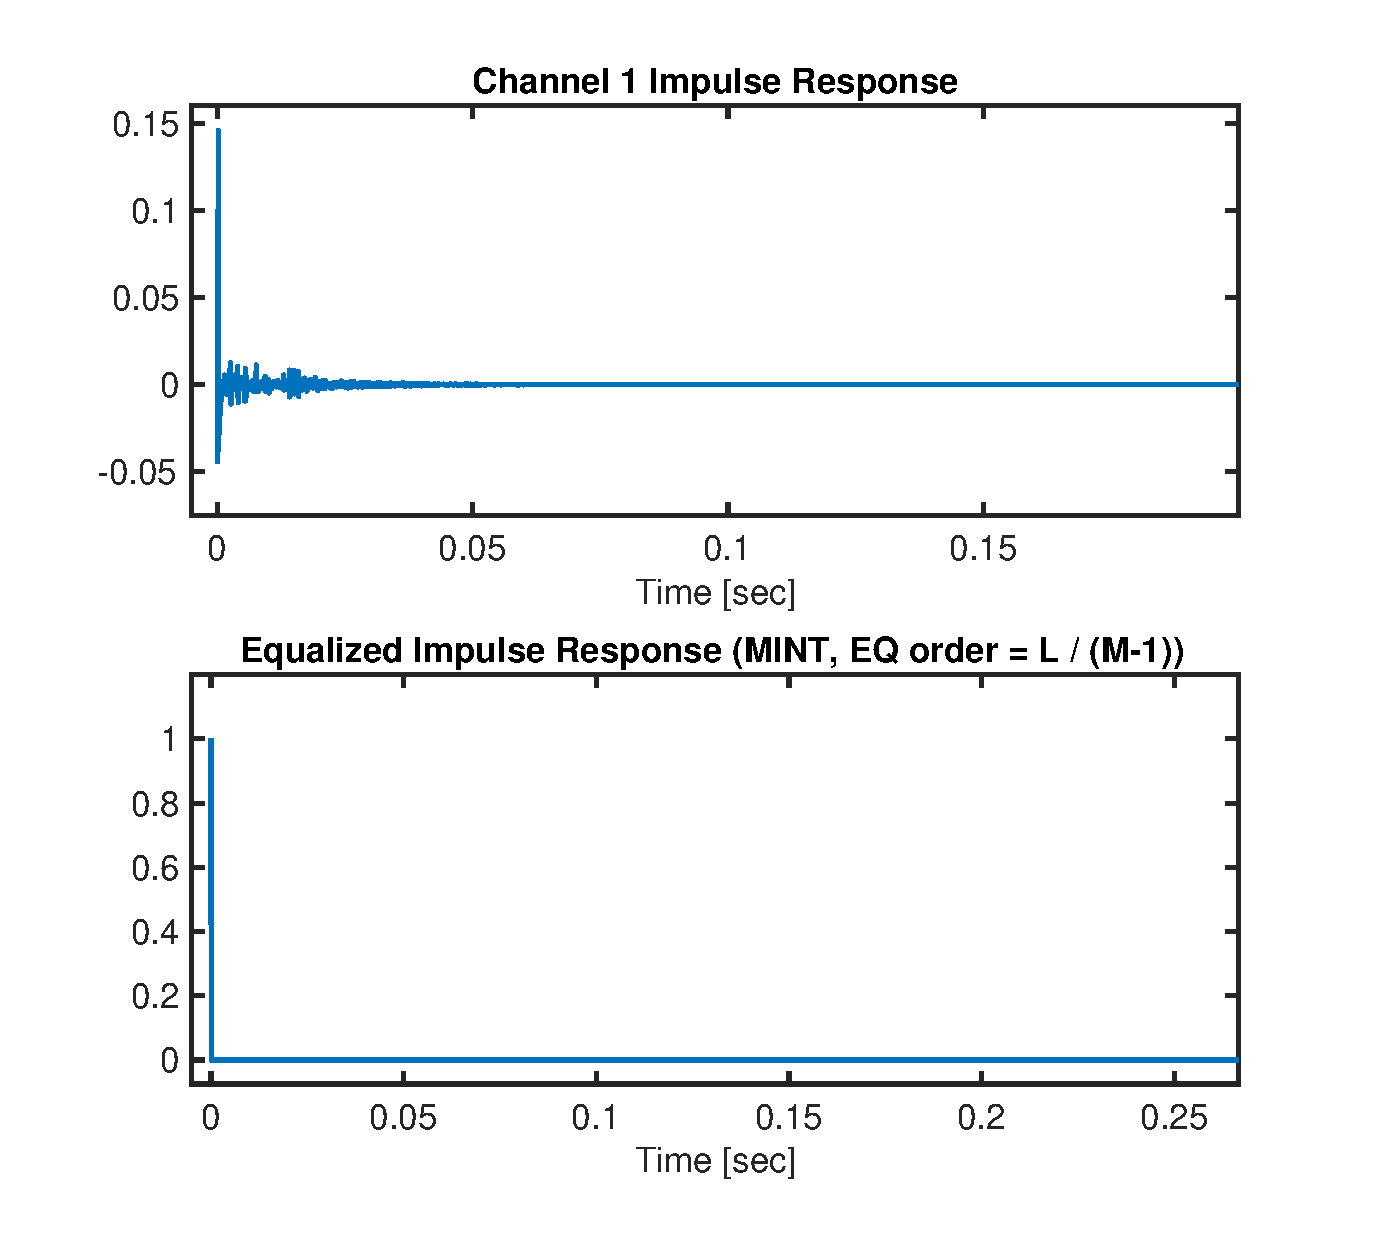
\includegraphics[width=\linewidth]{MINT_EIR_L_div_M_minus_1}
			\end{subfigure}
			\hfill
			\begin{subfigure}[t]{0.49\textwidth}
				\centering
				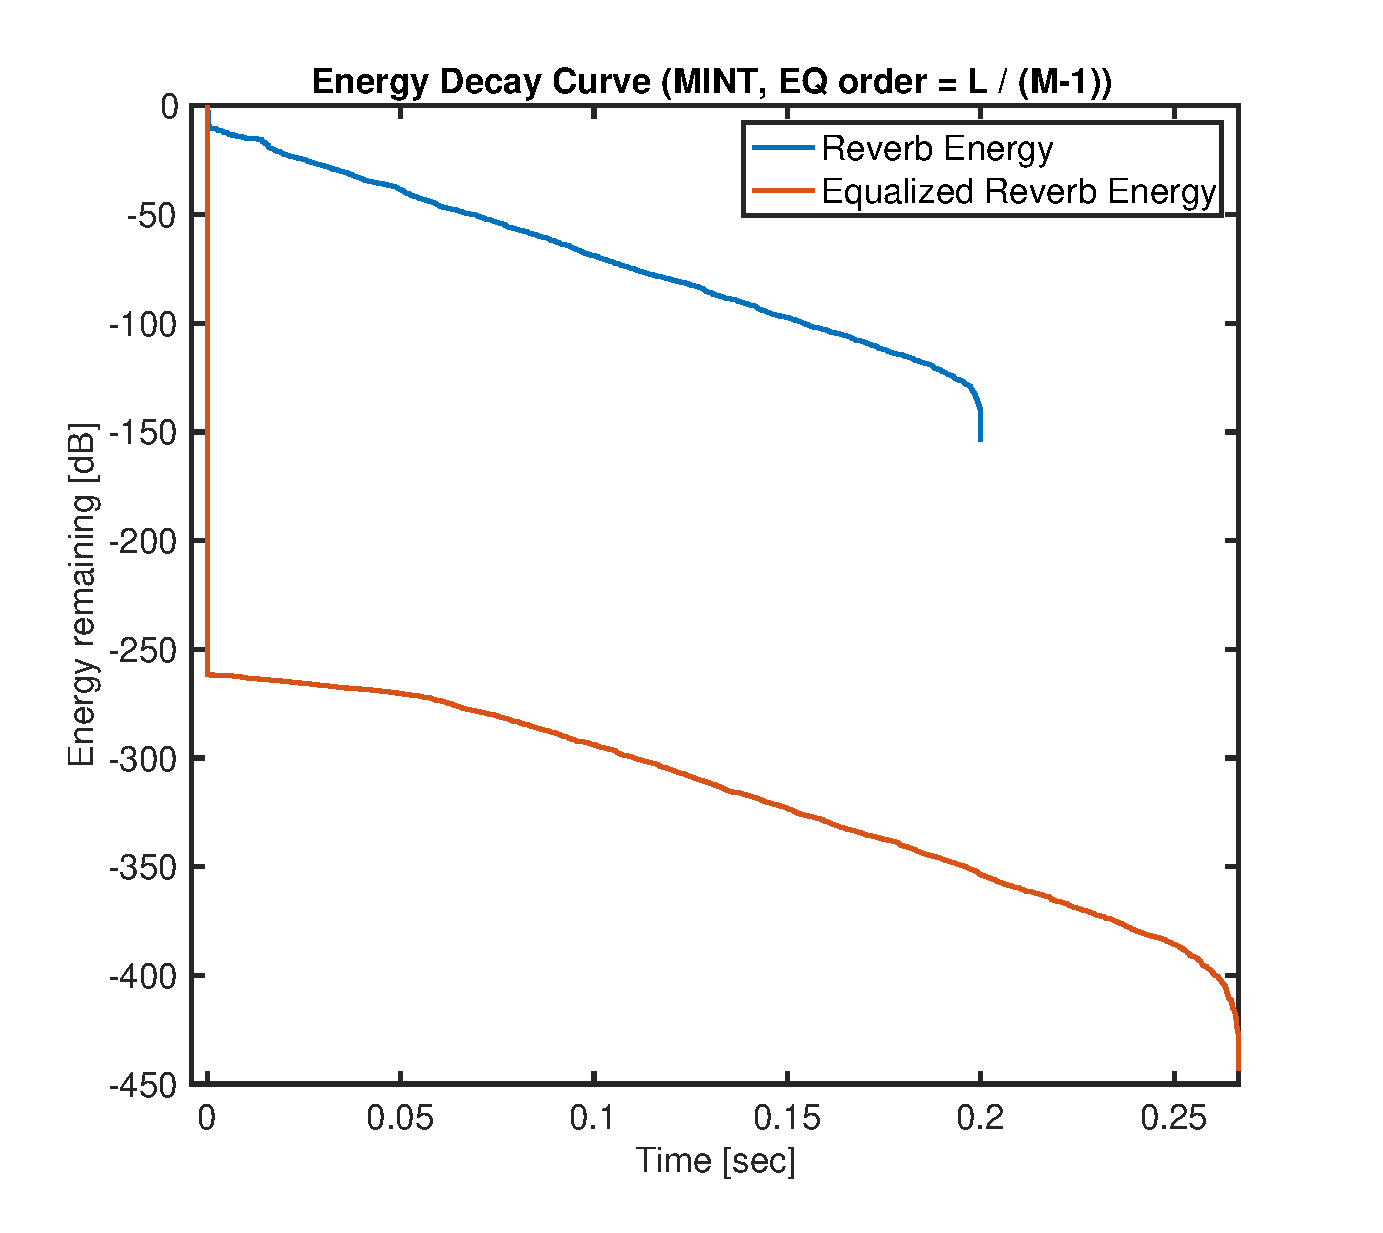
\includegraphics[width=\linewidth]{MINT_EDC_L_div_M_minus_1}
			\end{subfigure}
		\end{minipage}
	}
	% Dummy subfigure for referencing row A
	\refstepcounter{subfigure}
	\label{subfig:params_p2_MINT_compare:A}
	
	\vspace{1em}
	
	% ROW B
	\makebox[\textwidth][l]{%
		\begin{minipage}{0.23\textwidth}
			\centering
			\raggedleft{\footnotesize \textbf{(b)} \newline $p_2 = \mathrm{N60}  / (M-1)$} \\
		\end{minipage}%
		\begin{minipage}{0.675\textwidth}
			\begin{subfigure}[t]{0.49\textwidth}
				\centering
				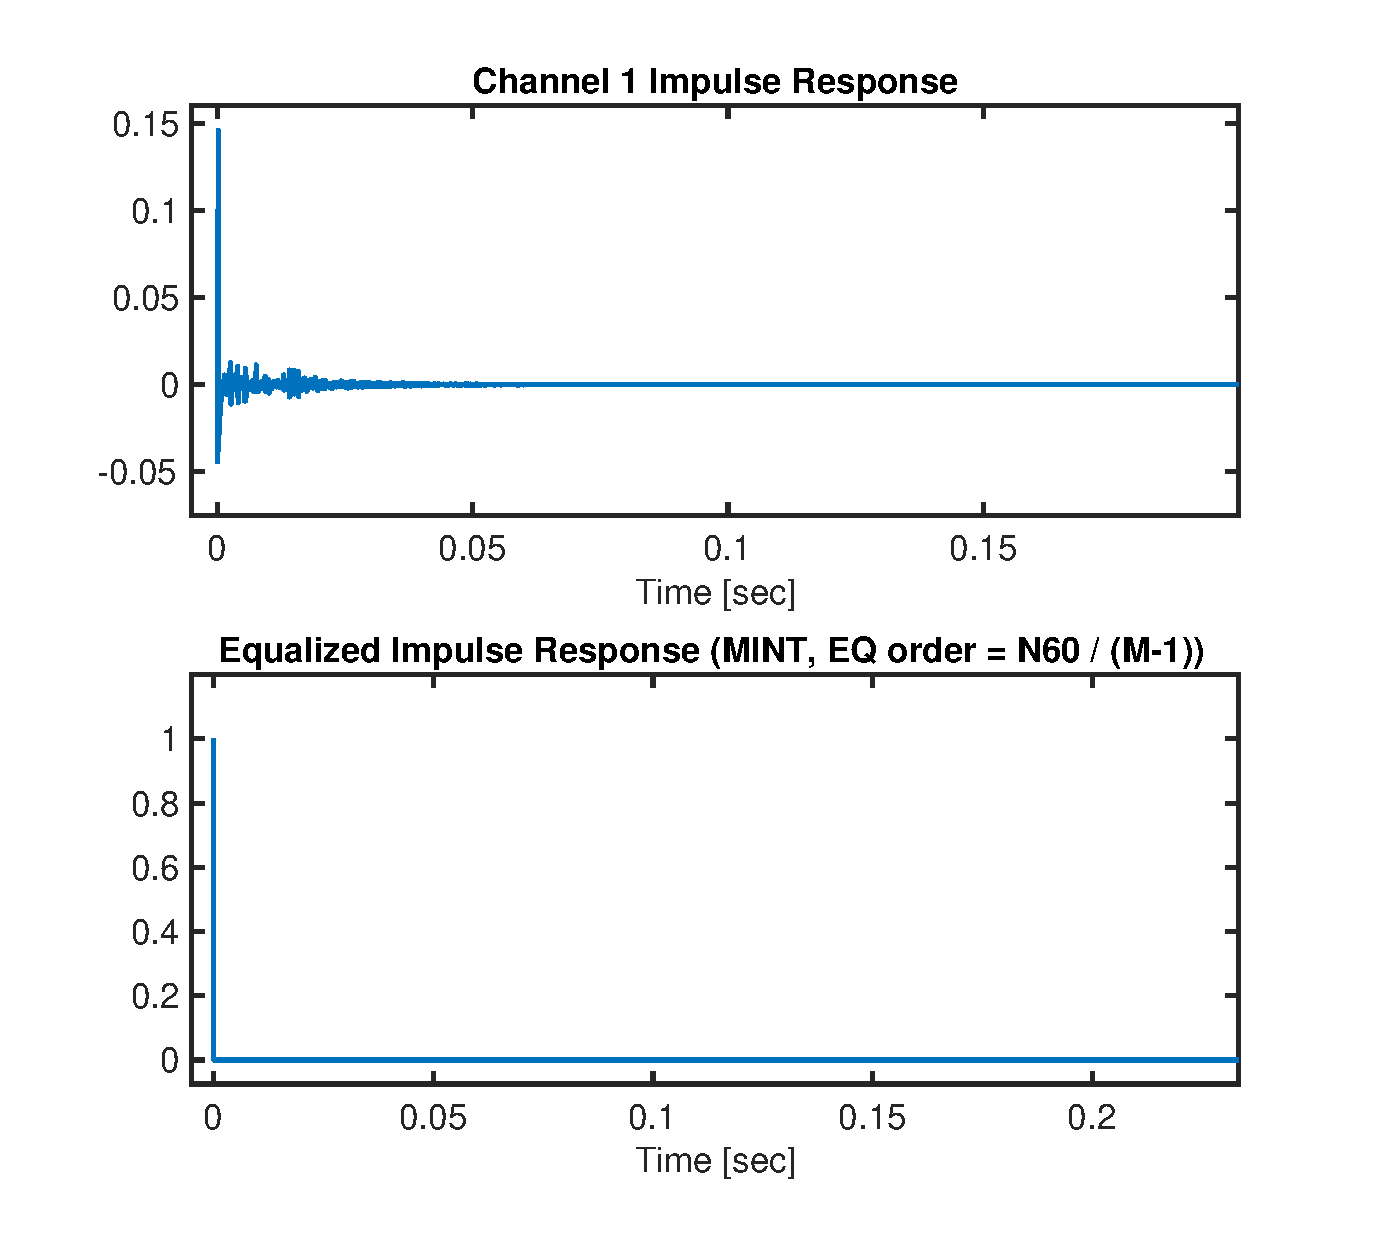
\includegraphics[width=\linewidth]{MINT_EIR_N60_div_M_minus_1}
			\end{subfigure}
			\hfill
			\begin{subfigure}[t]{0.49\textwidth}
				\centering
				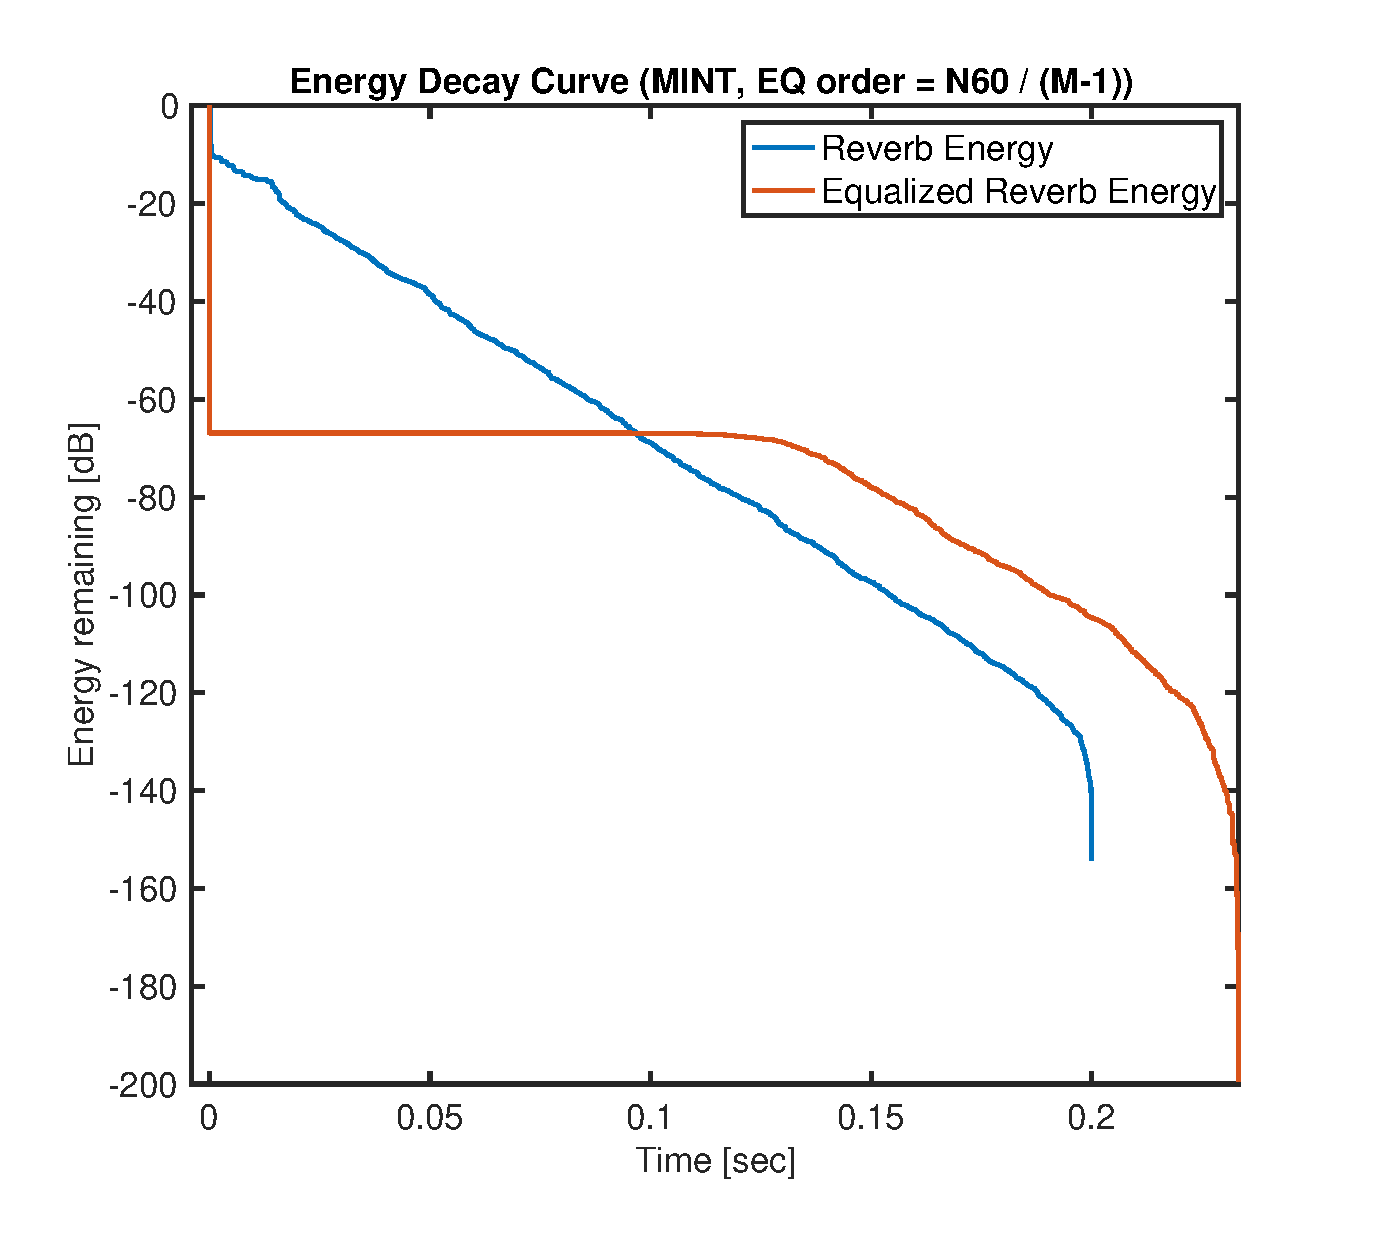
\includegraphics[width=\linewidth]{MINT_EDC_N60_div_M_minus_1}
			\end{subfigure}
		\end{minipage}
	}
	% Dummy subfigure for referencing row B
	\refstepcounter{subfigure}
	\label{subfig:params_p2_MINT_compare:B}
	
	\vspace{1em}
	
	% ROW C
	\makebox[\textwidth][l]{%
		\begin{minipage}{0.23\textwidth}
			\centering
			\raggedleft{\footnotesize \textbf{(c)} \newline $p_2 = 0.75 \cdot \mathrm{N60}  / (M-1)$} \\
		\end{minipage}%
		\begin{minipage}{0.675\textwidth}
			\begin{subfigure}[t]{0.49\textwidth}
				\centering
				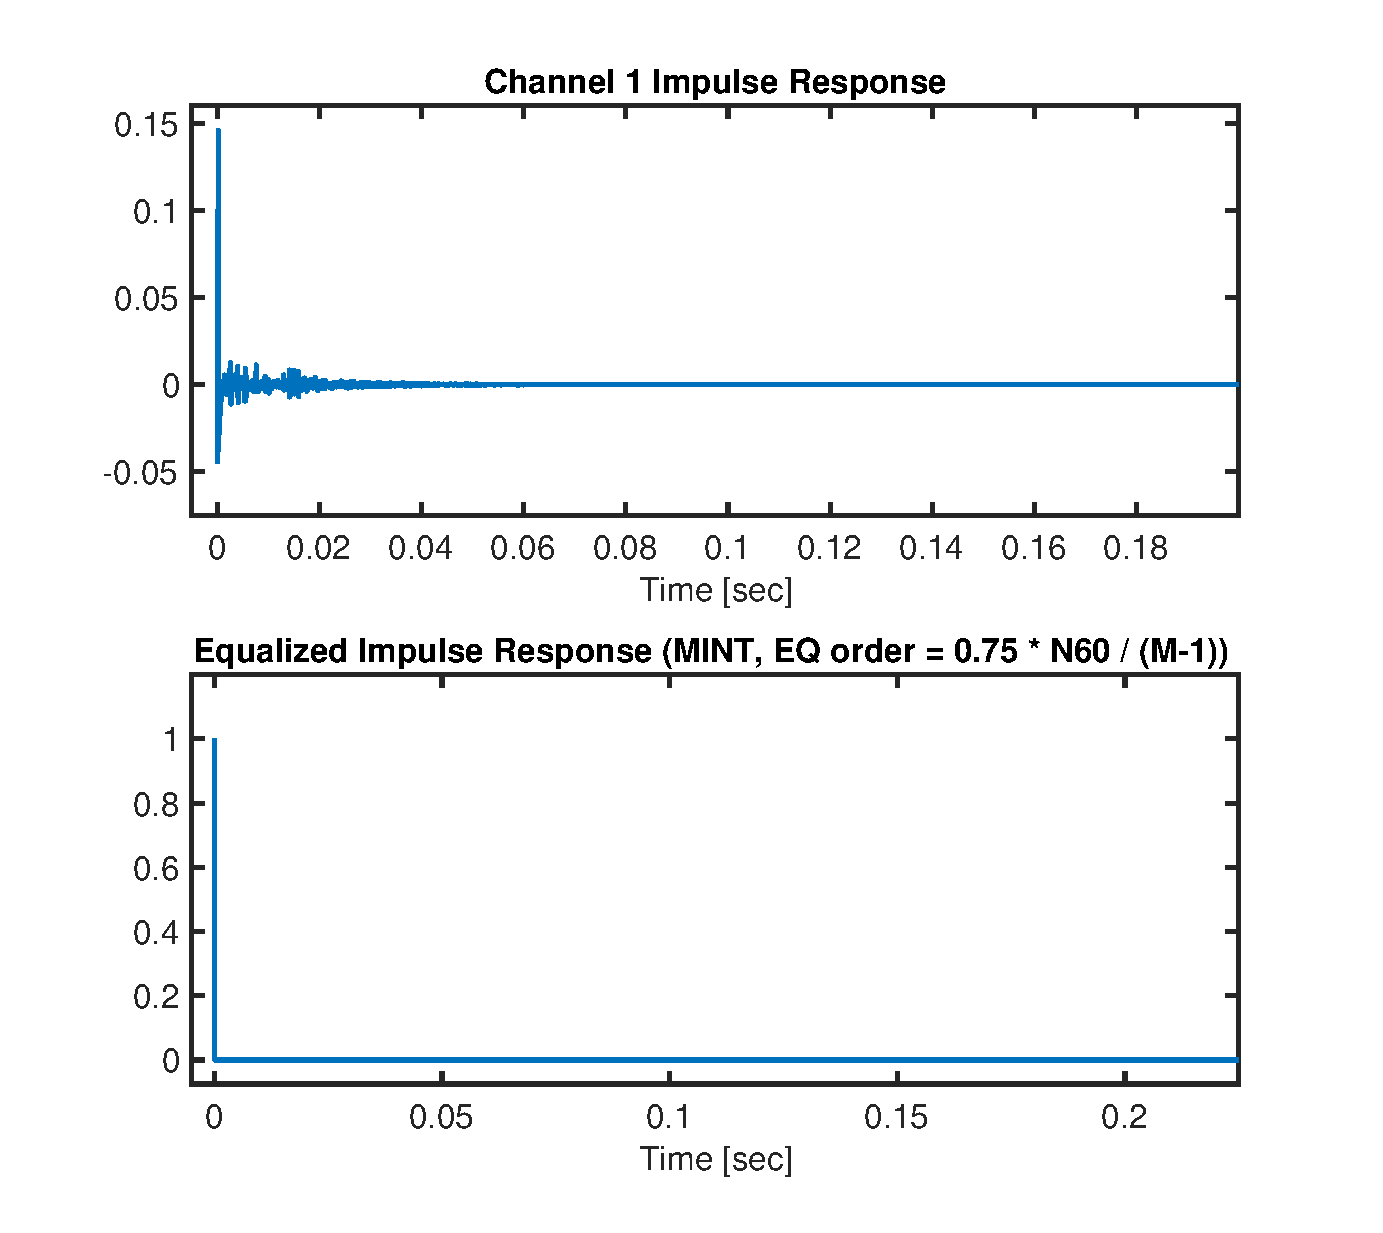
\includegraphics[width=\linewidth]{MINT_EIR_0p75N60_div_M_minus_1}
			\end{subfigure}
			\hfill
			\begin{subfigure}[t]{0.49\textwidth}
				\centering
				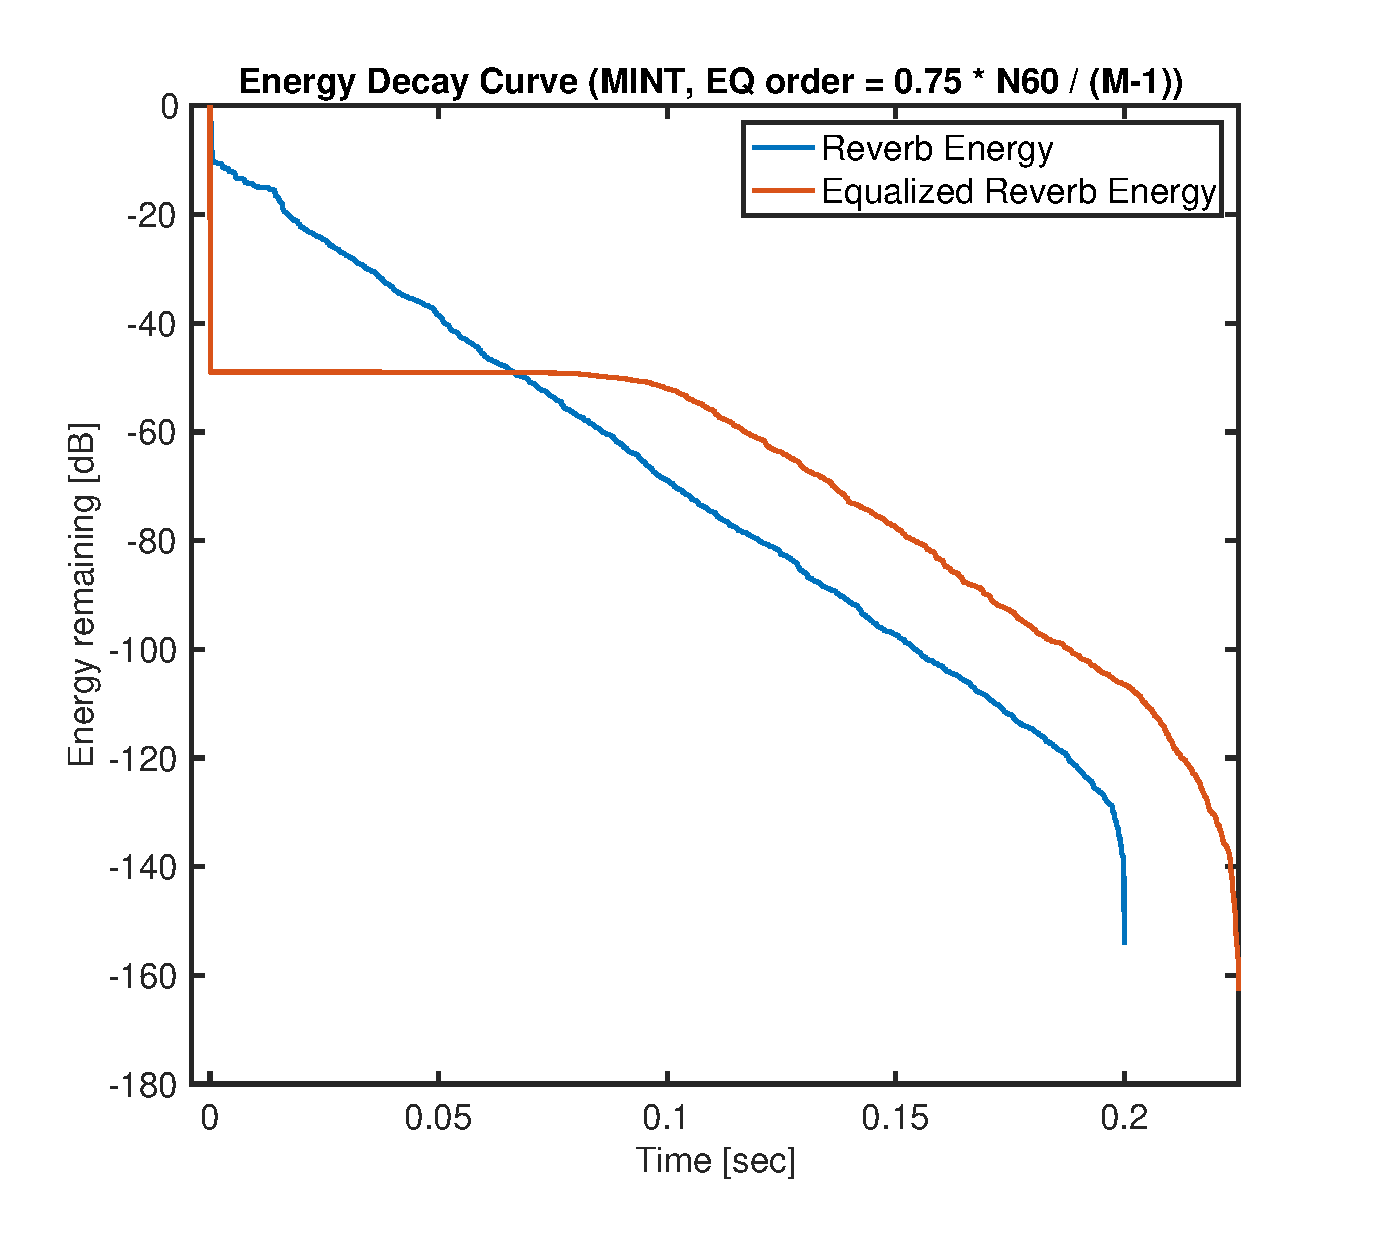
\includegraphics[width=\linewidth]{MINT_EDC_0p75N60_div_M_minus_1}
			\end{subfigure}
		\end{minipage}
	}
	% Dummy subfigure for referencing row C
	\refstepcounter{subfigure}
	\label{subfig:params_p2_MINT_compare:C}
	
	\vspace{1em}
	
	% ROW D
	\makebox[\textwidth][l]{%
		\begin{minipage}{0.23\textwidth}
			\centering
			\raggedleft{\footnotesize \textbf{(d)} \newline $p_2 = 0.5 \cdot \mathrm{N60} / (M-1)$} \\
		\end{minipage}%
		\begin{minipage}{0.675\textwidth}
			\begin{subfigure}[t]{0.49\textwidth}
				\centering
				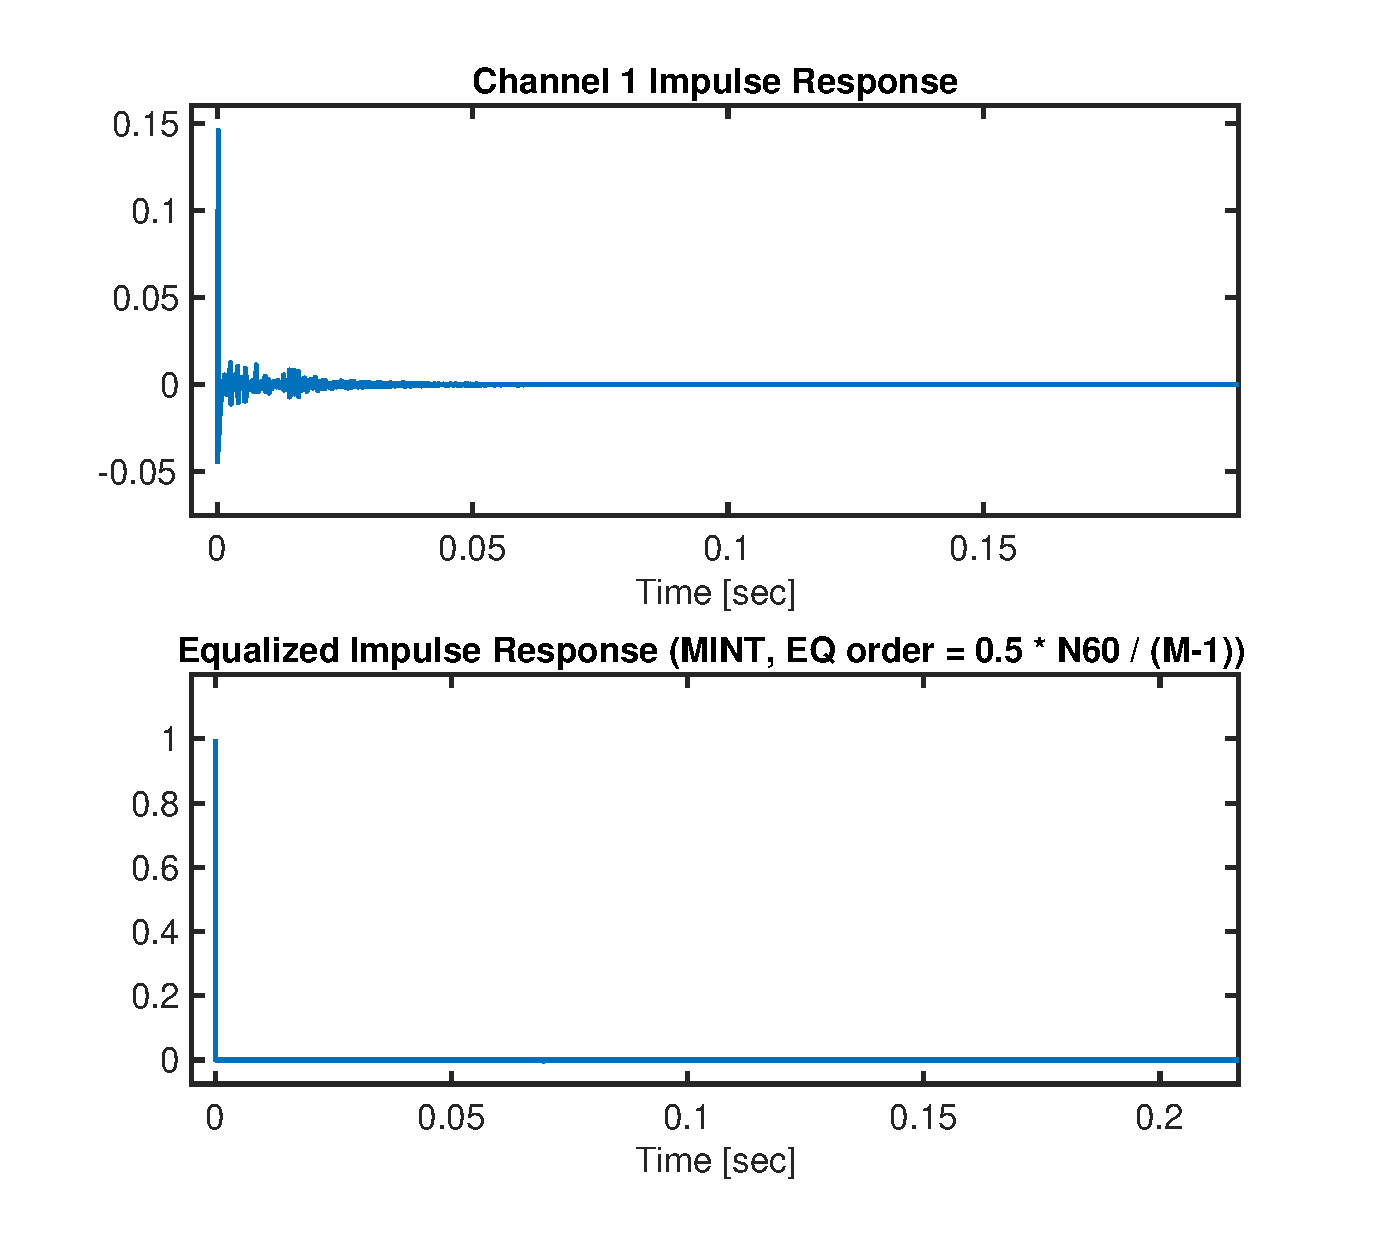
\includegraphics[width=\linewidth]{MINT_EIR_0p5N60_div_M_minus_1}
			\end{subfigure}
			\hfill
			\begin{subfigure}[t]{0.49\textwidth}
				\centering
				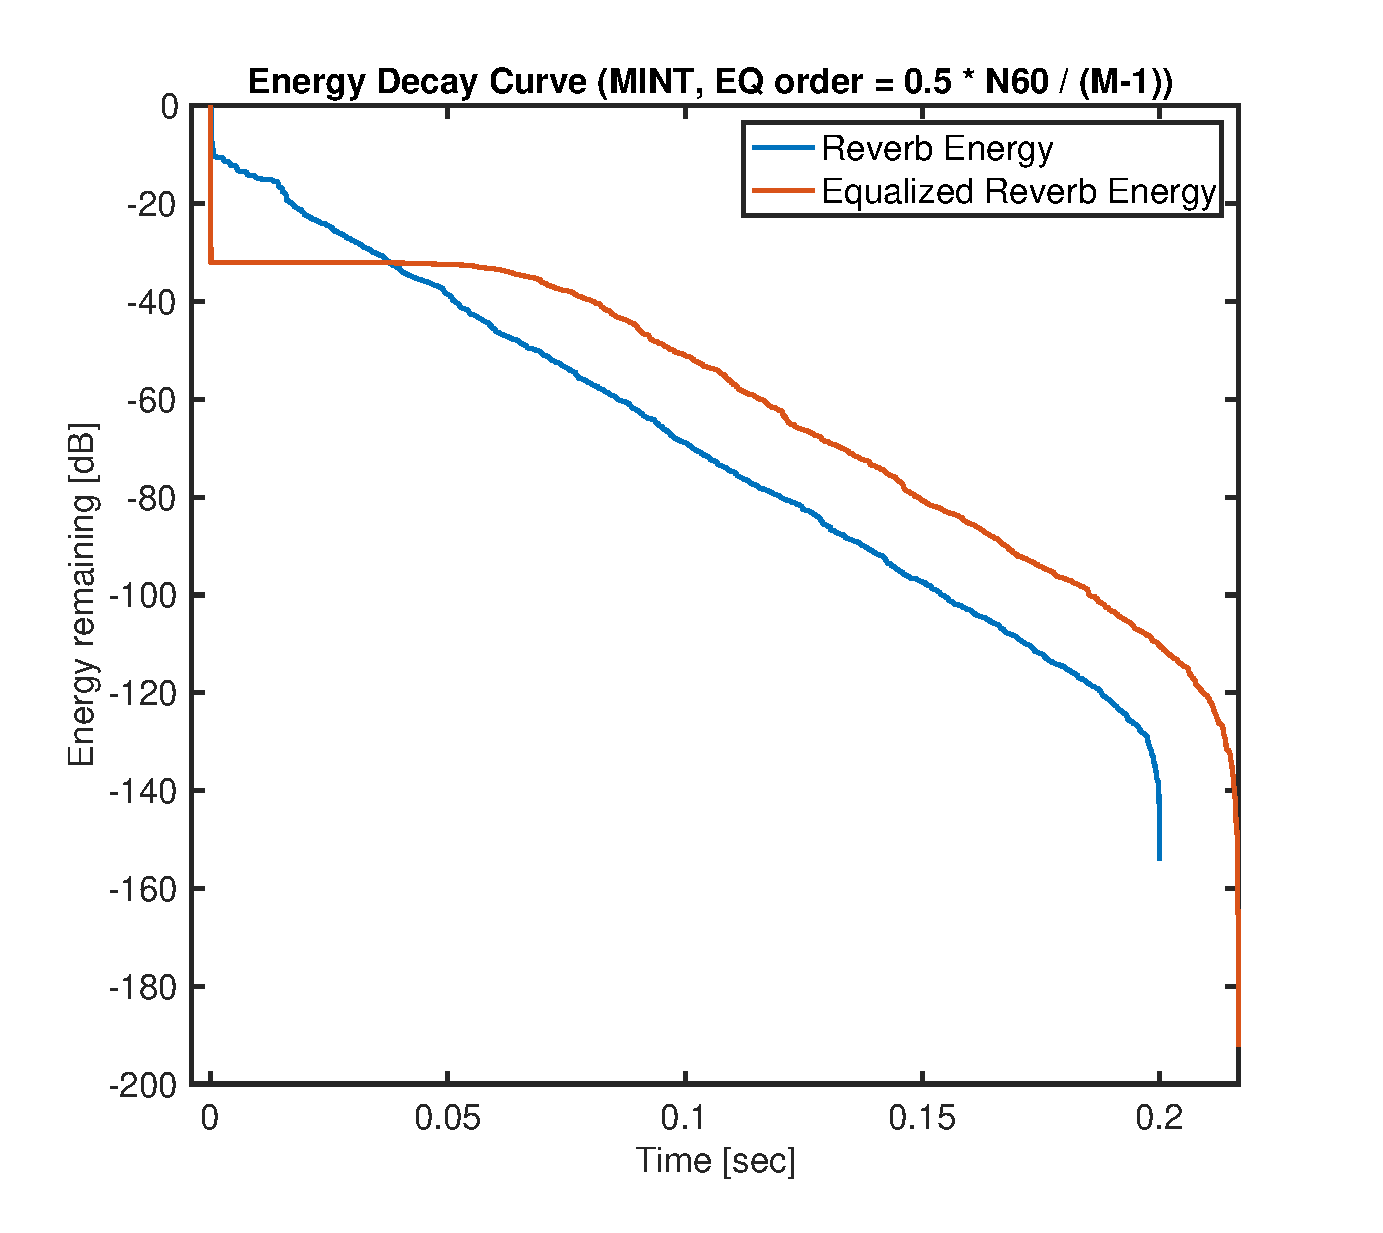
\includegraphics[width=\linewidth]{MINT_EDC_0p5N60_div_M_minus_1}
			\end{subfigure}
		\end{minipage}
	}
	% Dummy subfigure for referencing row D
	\refstepcounter{subfigure}
	\label{subfig:params_p2_MINT_compare:D}
	
	\caption[MINT equalizer performance for various filter orders]{MINT equalizer performance for various equalizer orders. Equalizer orders ($p_2$) are quantified relative to the actual length of the FIR channel ($L$) and the number of samples corresponding to the T60 of the channel ($\mathrm{N60} = \mathrm{T60}  \cdot \mathrm{sample\ rate}$)}
	\label{fig:params_p2_MINT_compare}
	
\end{figure}

As expected, near-perfect equalization was acheived by the MINT for $p2 = L / \left(M-1\right)$, with the EDC decaying by $>$ \qty{250}{\decibel} almost instantaneously (Figure \ref{subfig:params_p2_MINT_compare:A}). Similarly, when the T60 was used to set the equalizer length rather than the actual FIR RIR length, the EDC decayed by about approximately 60 dB almost instaneously (Figure \ref{subfig:params_p2_MINT_compare:B}). As the equalizer length was decreased relative to the T60, the EDC performance of the MINT dropped substantially. Based on these observations, The $p_2$ should be selected such that it is possible to acheive the amount of attenuation desired. If the goal is to reduce the T60, $p_2 = \mathrm{N60}  / \left(M-1 \right)$ is sufficient.

\subsection{Multichannel Linear Prediction Inverse Filtering Results} \label{section:params_p2_MC_LP} 

To analyze the behavior of the MC-LP of the DAP algorithm stage in isolation, without the performance impact of blindly estimating the AR properties of the source signal, the source-whitening stage was trained on the clean speech signal (i.e., supervised estimation of AR properties). One might suggest instead using a white noise sequence as the source signal and bypassing the source whitening stage altogether, but it was found that due to the high frequency resolution of the high-order MC-LP stage, the ripples in the specific realization of the uncorrelated random process would be whitened thus distorting the estimate of the true multichannel RTF inverse. The same MC-LP orders ($p_2$) were evaluated as were compared in Figure \ref{fig:params_p2_MINT_compare}. A source-whitening prediction order of $p_1 = 4000$ was used accross all cases. The sample rate was \qty{16}{\kilo\hertz}, the source signal was \qty{21.8}{\sec} of speech taken from the TMIT speech sample database \citep{garofolo1993timit}. The same four RIRs were used as in the previous section. The RIRs were manually time aligned, and the non-zero measurement noise samples leading the direct sound were manually set to zero. If leading measurement noise were not removed from the RIRs, these noise samples would be convolved with the source signal in simulation as though they were real reflections that lead the direct sound. The MC-LP stage will always equalize to the first non-zero impulse because later impulses will be predictable from previous ones and therefore will be cancelled. Leaving the leading measurement noise samples would have an unrealistic negative impact on dereverberation performance since these samples are small relative to the actual RIR and thus also small relative to the residual reverberation left un-cancelled by the algorithm.

The results of the source-whitening stage that was common throughout this experiment are shown in Figure \ref{fig:params_p2_stage1}. The top pane shows the estimated source spectrum (i.e., the LP inverse filter) compared to the true power spectrum of the clean source signal in the first pane and the second pane shows resulting whitened power spectrum of the clean source signal, which was generated by applying the source-whitening filter to the clean speech signal instead of the reverberant speech. The EIRs and EDCs resulting from the MC-LP stage for each prediction order are shown in Figure \ref{fig:params_p2_compare}. For more detailed plots of the inner-workings of the algorithm in this evaluation, refer to Appendix \ref{section:appendix:params_p2}. 

% Test Conditions for all:
% - Source Signal = SA1.WAV
% - Source length = 348366
% - RIR = MYRiAD SAL Measured RIR (T60 = 2100 msec, Truncated Exponentially to T60 = 100 msec)
% - RIR length = 3200
% - T60 = 100 msec (N60 = 1600 samples)
% - SNR = 300 dB
% - Noise Signal = office ventilation
% - SIR = Inf dB
% - Interference Signal = None
%
% Delay-and-Predict config:
% - Number of Microphones (M) = 4
% - Source whitening order (p1) = 4000
% - Multichannel Linear Prediction order (p2) = varied
% - Source whitening Enabled? = 1
% - Source whitening on clean speech? = 1


\begin{figure}[H]
	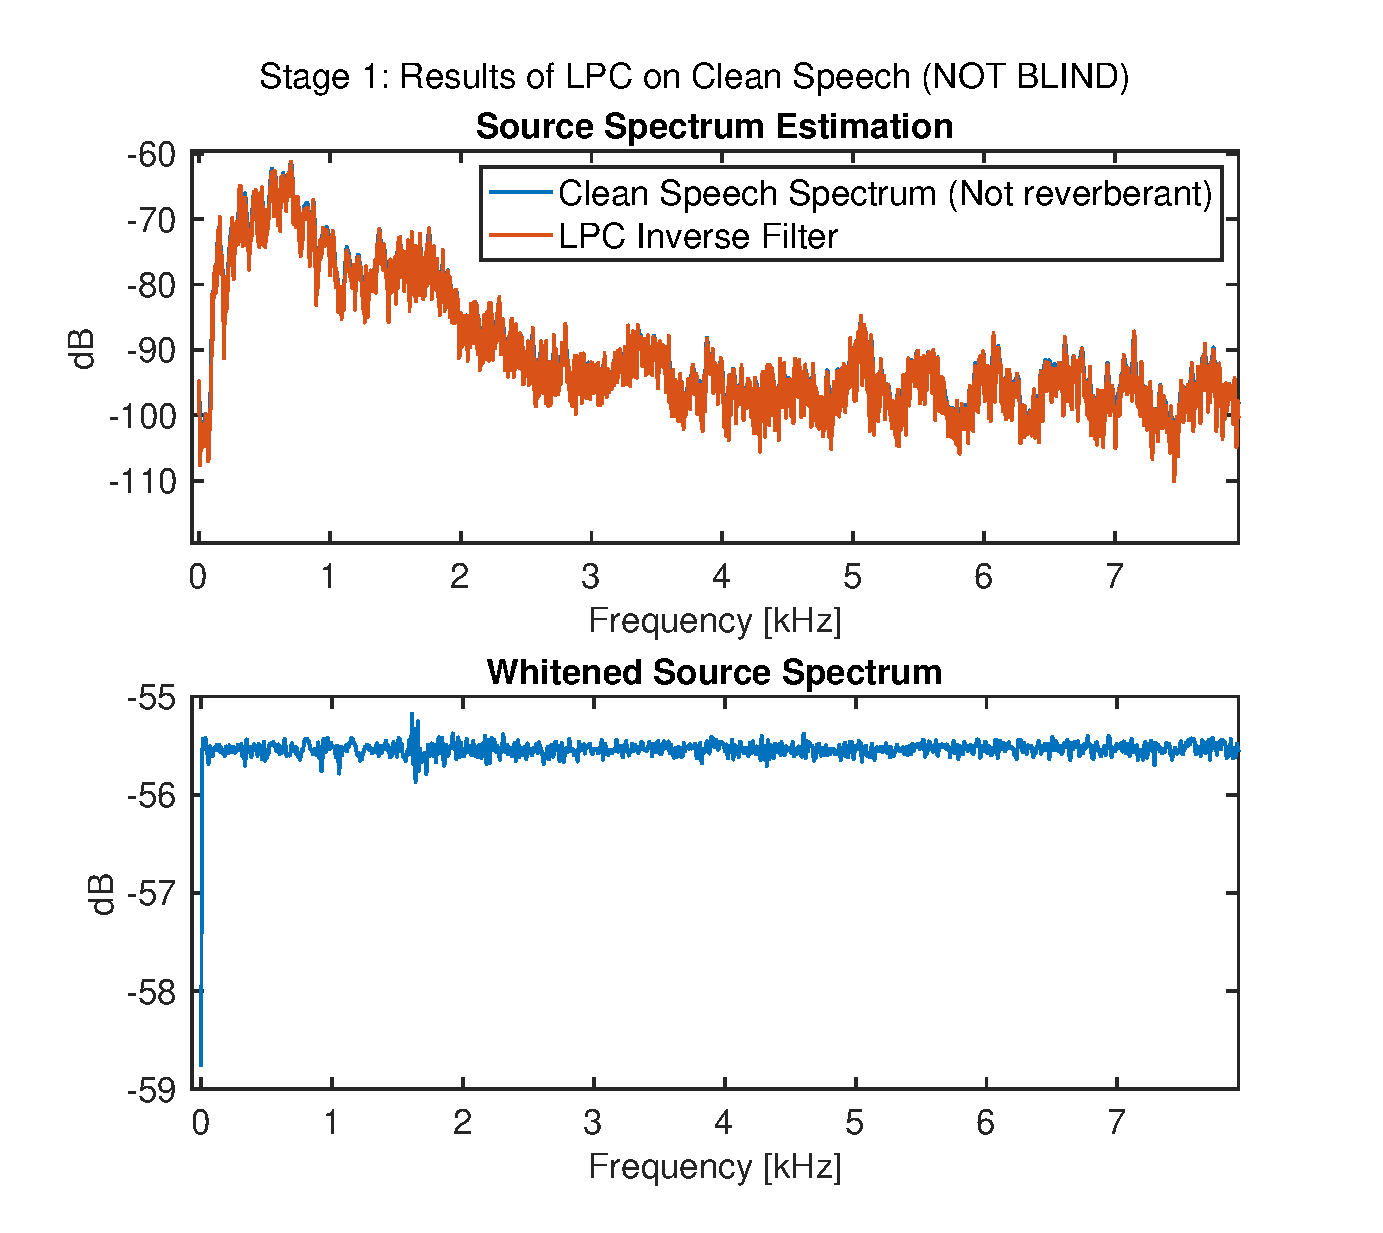
\includegraphics[width=0.49\textwidth]{S1_N60_div_M_minus_1}
	\centering
	\caption[Source whitening results used in analysis of DAP dereverberation performance for various MC-LP orders]{Source whitening results using a $\mathrm{p1} = 4000$ order linear predictor. The prediction error filter coefficients were computed based on clean speech and the same filter was used in all tests in this section to assess the MC-LP stage of the DAP algorithm in isolation.}
	\label{fig:params_p2_stage1}
\end{figure}


\begin{figure}[H]
	\centering
	
	% ROW A
	\makebox[\textwidth][l]{%
		\begin{minipage}{0.23\textwidth}
			\centering
			\raggedleft{\footnotesize \textbf{(a)} \newline $p_2 = L / (M-1)$} \\
		\end{minipage}%
		\begin{minipage}{0.66\textwidth}
			\begin{subfigure}[t]{0.49\textwidth}
				\centering
				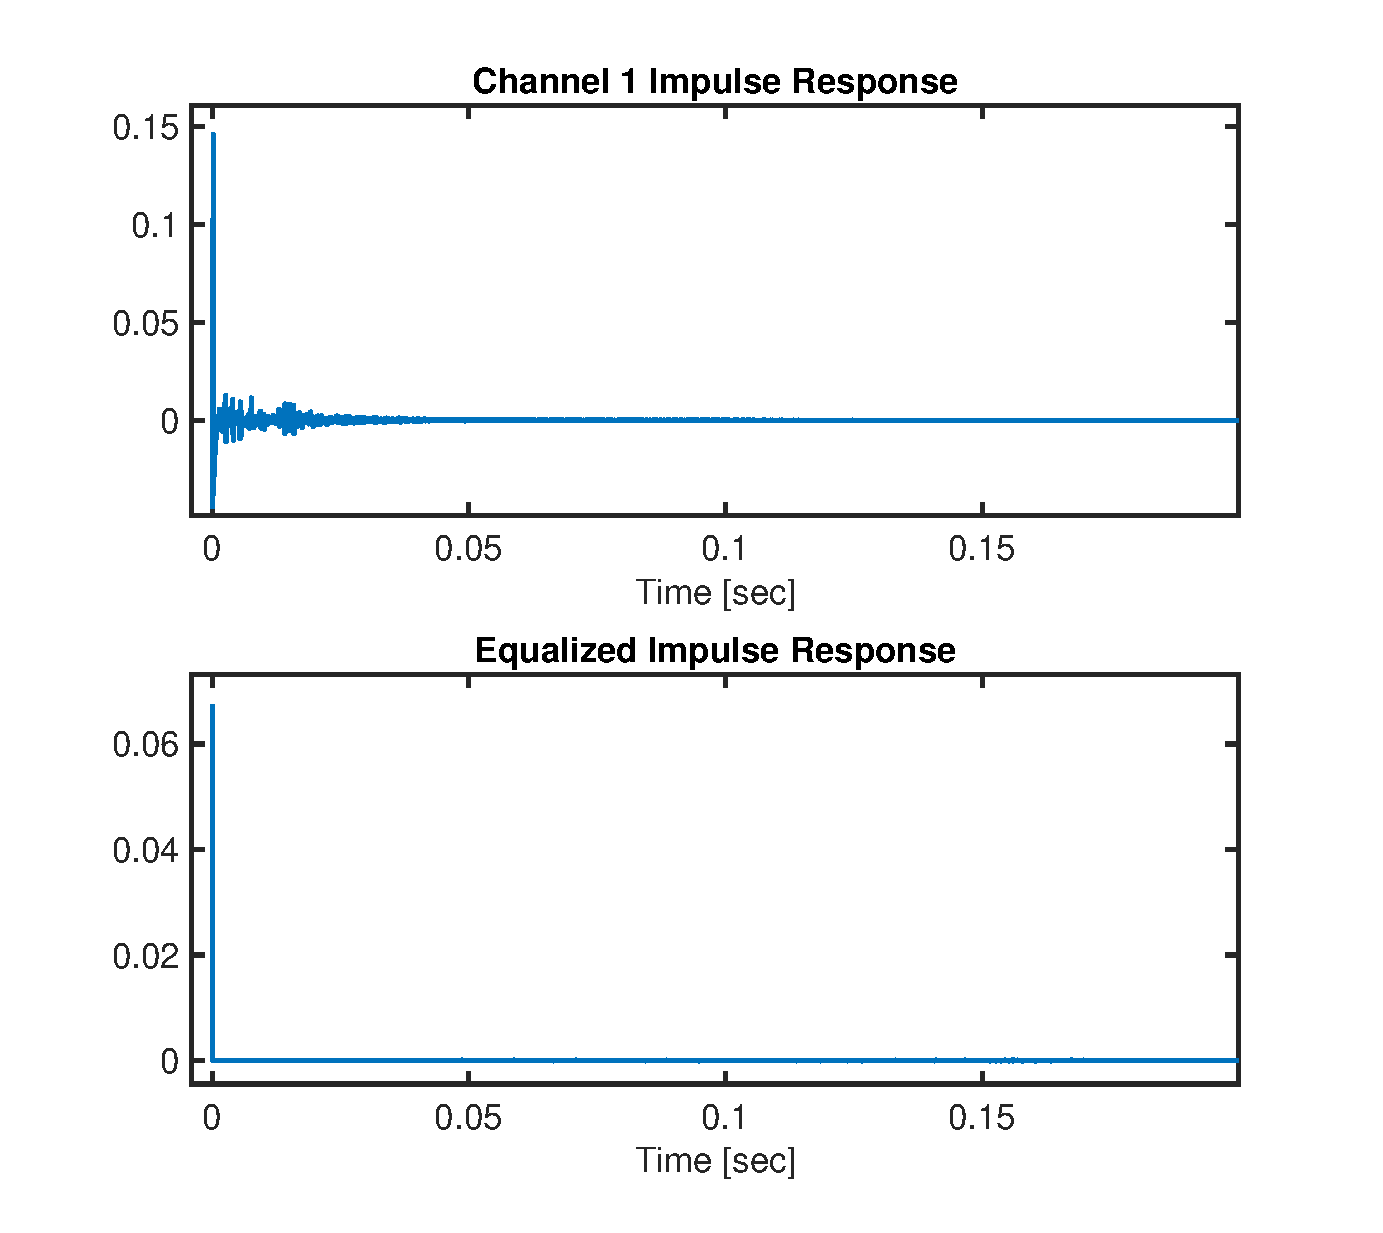
\includegraphics[width=\linewidth]{EIR_L_div_M_minus_1}
			\end{subfigure}
			\hfill
			\begin{subfigure}[t]{0.49\textwidth}
				\centering
				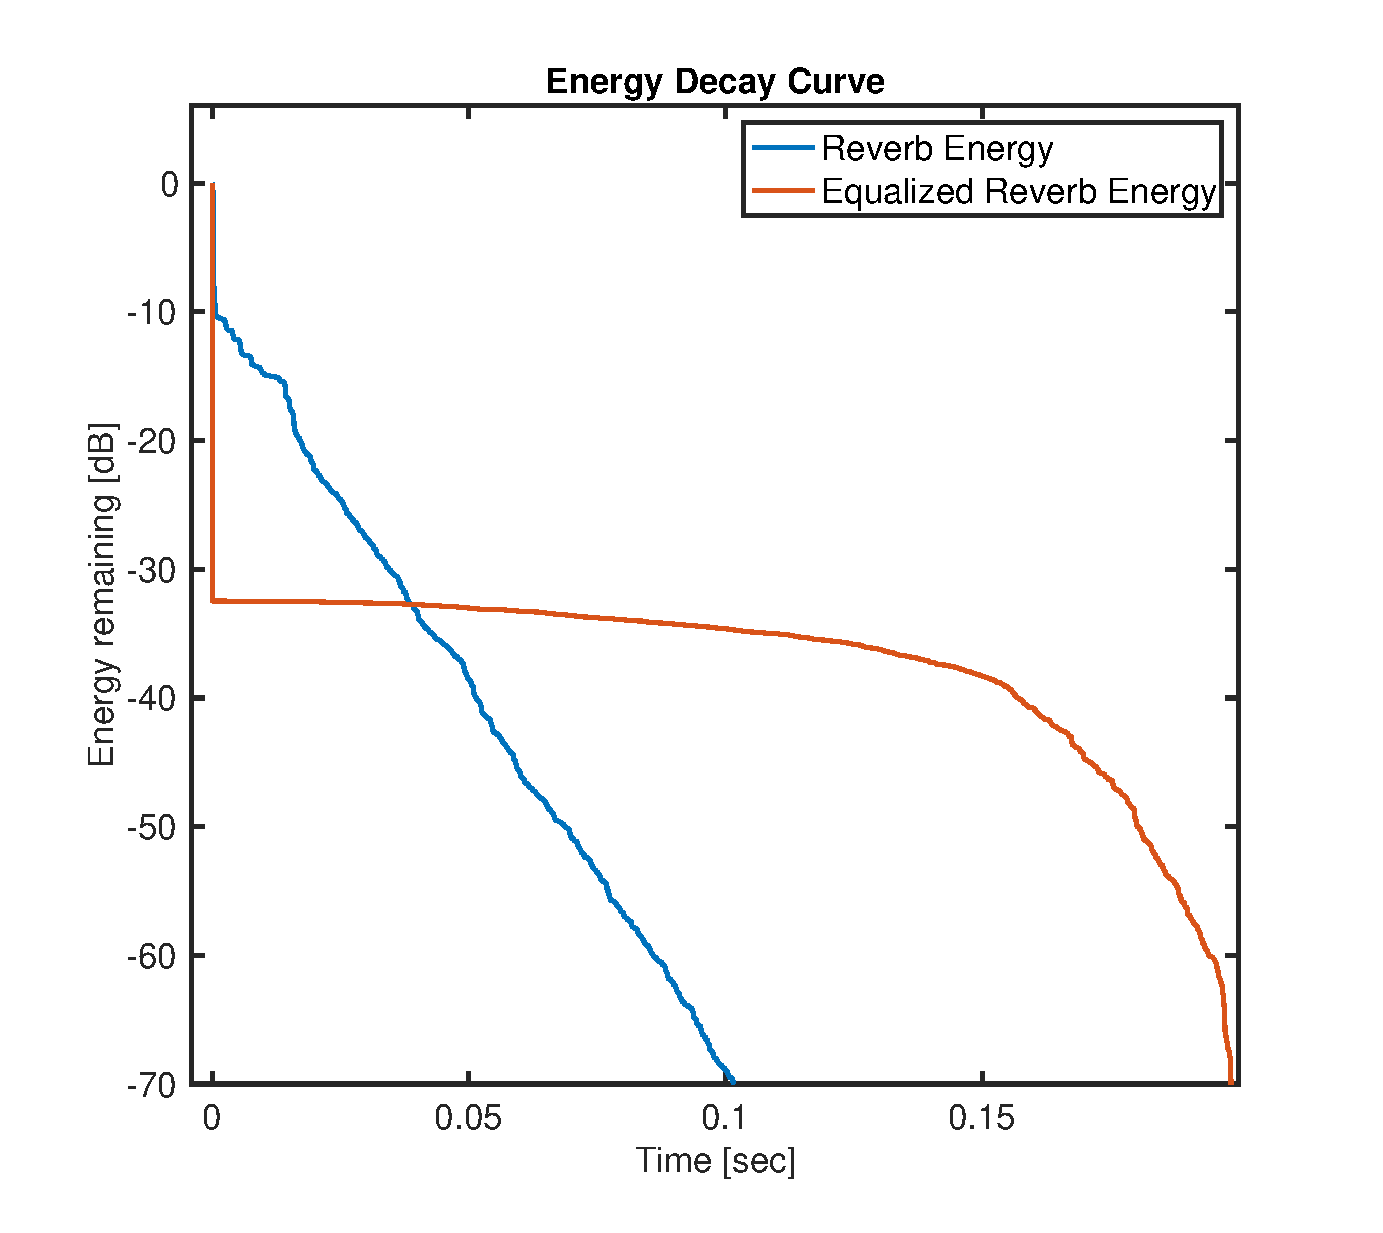
\includegraphics[width=\linewidth]{EDC_L_div_M_minus_1}
			\end{subfigure}
		\end{minipage}
	}
	% Dummy subfigure for referencing row A
	\refstepcounter{subfigure}
	\label{subfig:params_p2_compare:A}
	
	\vspace{1em}
	
	% ROW B
	\makebox[\textwidth][l]{%
		\begin{minipage}{0.23\textwidth}
			\centering
			\raggedleft{\footnotesize \textbf{(b)} \newline $p_2 = \mathrm{N60}  / (M-1)$} \\
		\end{minipage}%
		\begin{minipage}{0.66\textwidth}
			\begin{subfigure}[t]{0.49\textwidth}
				\centering
				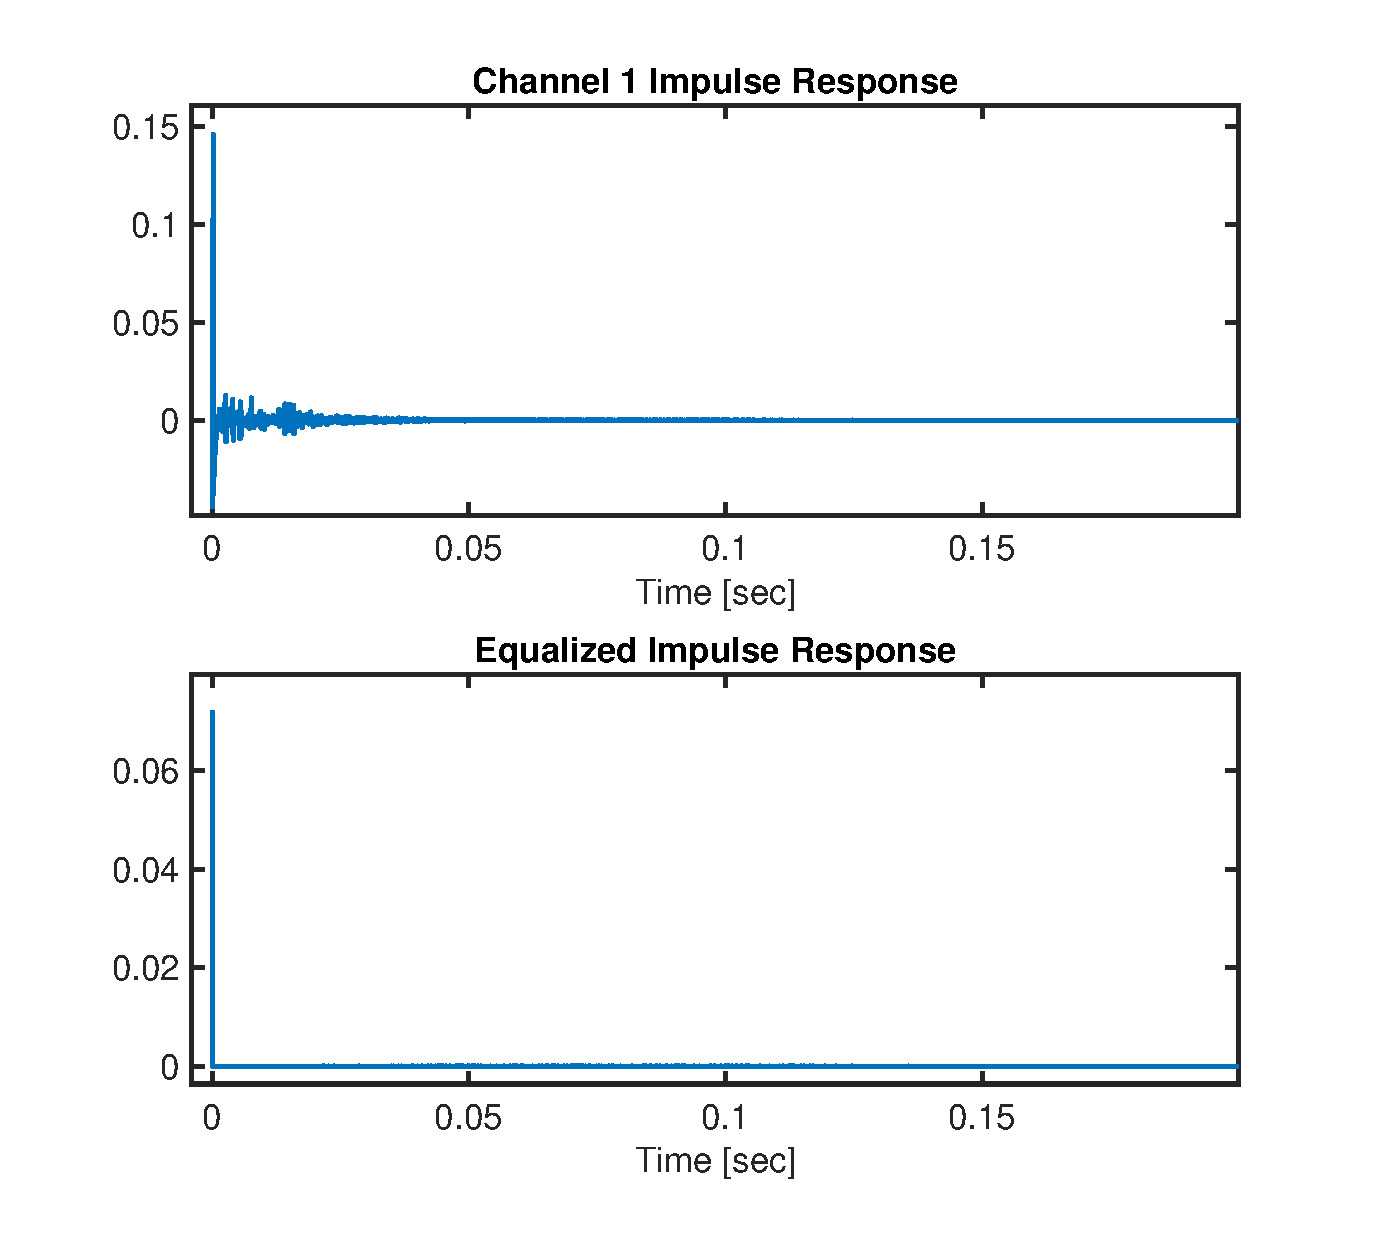
\includegraphics[width=\linewidth]{EIR_N60_div_M_minus_1}
			\end{subfigure}
			\hfill
			\begin{subfigure}[t]{0.49\textwidth}
				\centering
				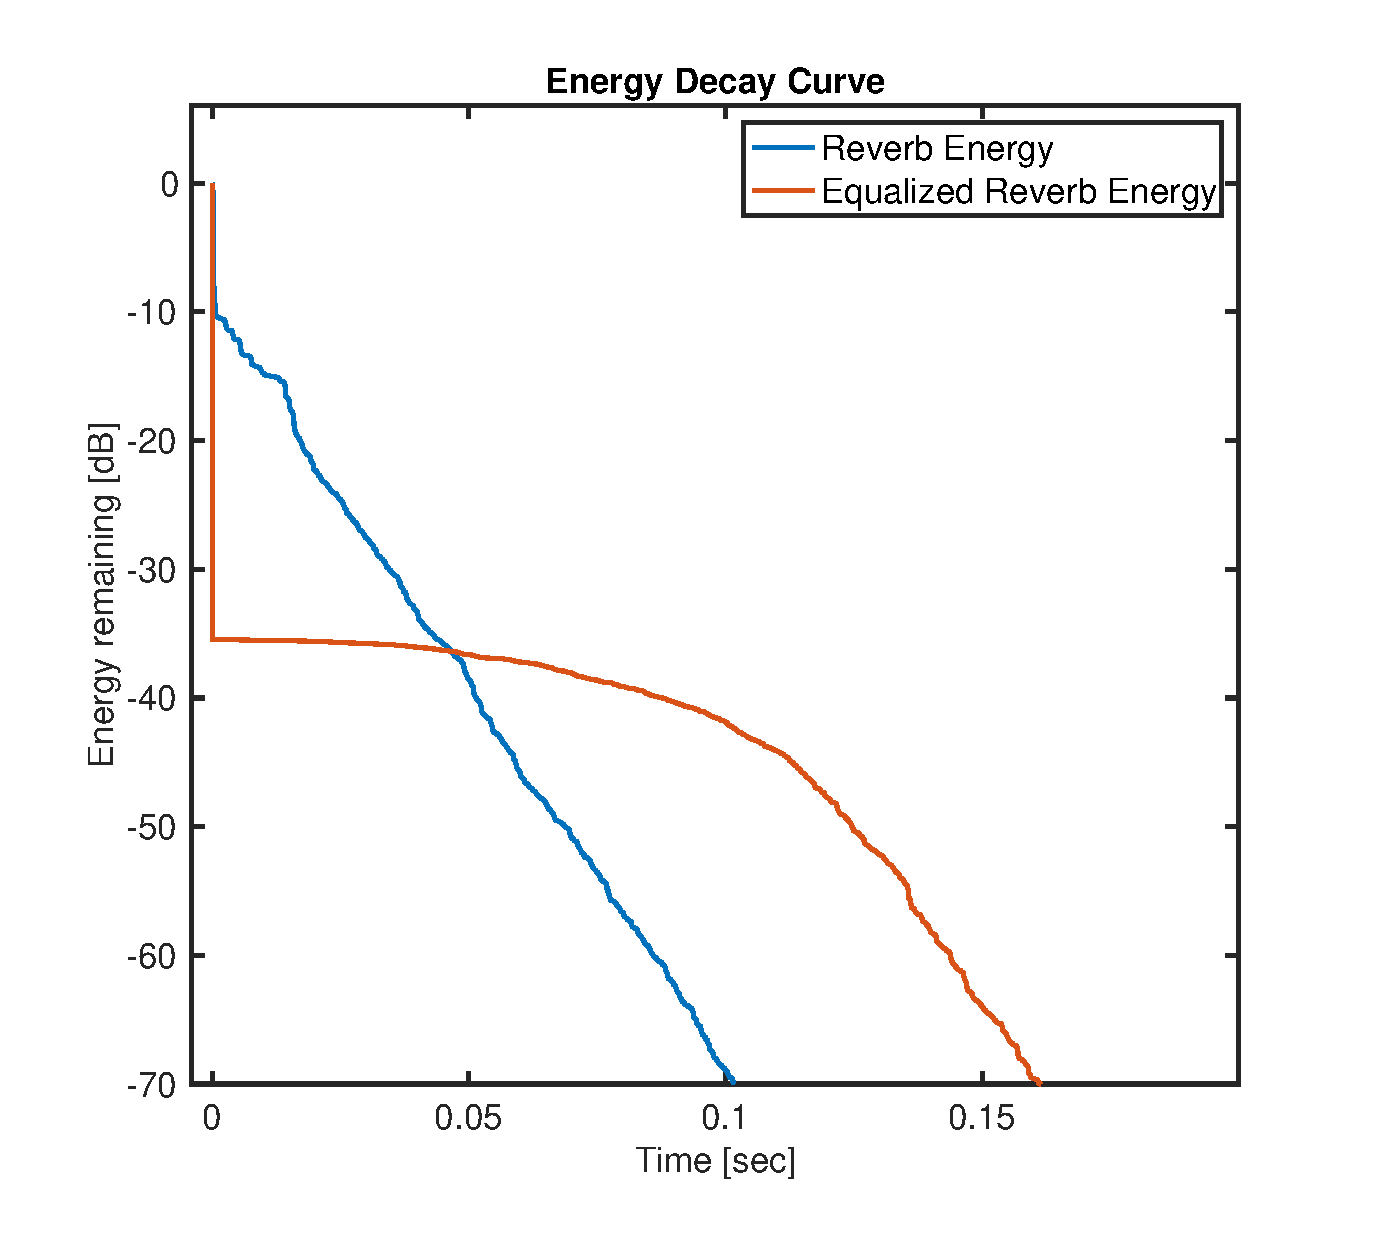
\includegraphics[width=\linewidth]{EDC_N60_div_M_minus_1}
			\end{subfigure}
		\end{minipage}
	}
	% Dummy subfigure for referencing row B
	\refstepcounter{subfigure}
	\label{subfig:params_p2_compare:B}
	
	\vspace{1em}
	
	% ROW C
	\makebox[\textwidth][l]{%
		\begin{minipage}{0.23\textwidth}
			\centering
			\raggedleft{\footnotesize \textbf{(c)} \newline $p_2 = 0.75 \cdot \mathrm{N60}  / (M-1)$} \\
		\end{minipage}%
		\begin{minipage}{0.66\textwidth}
			\begin{subfigure}[t]{0.49\textwidth}
				\centering
				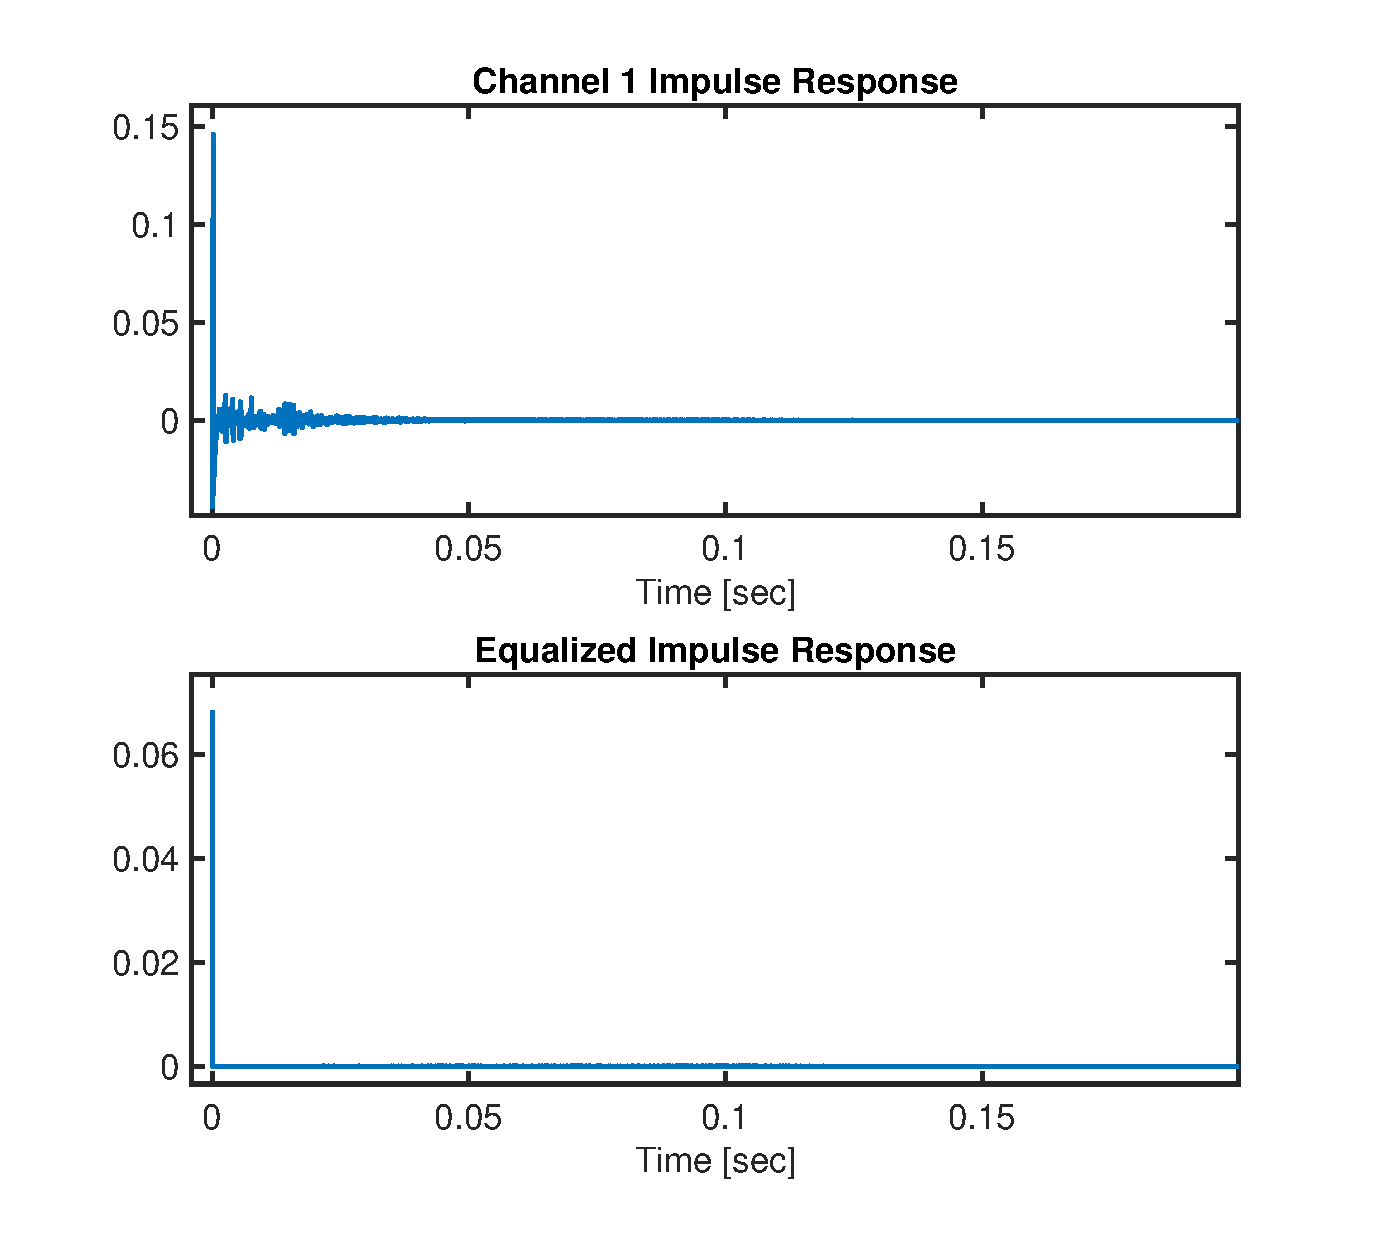
\includegraphics[width=\linewidth]{EIR_0p75N60_div_M_minus_1}
			\end{subfigure}
			\hfill
			\begin{subfigure}[t]{0.49\textwidth}
				\centering
				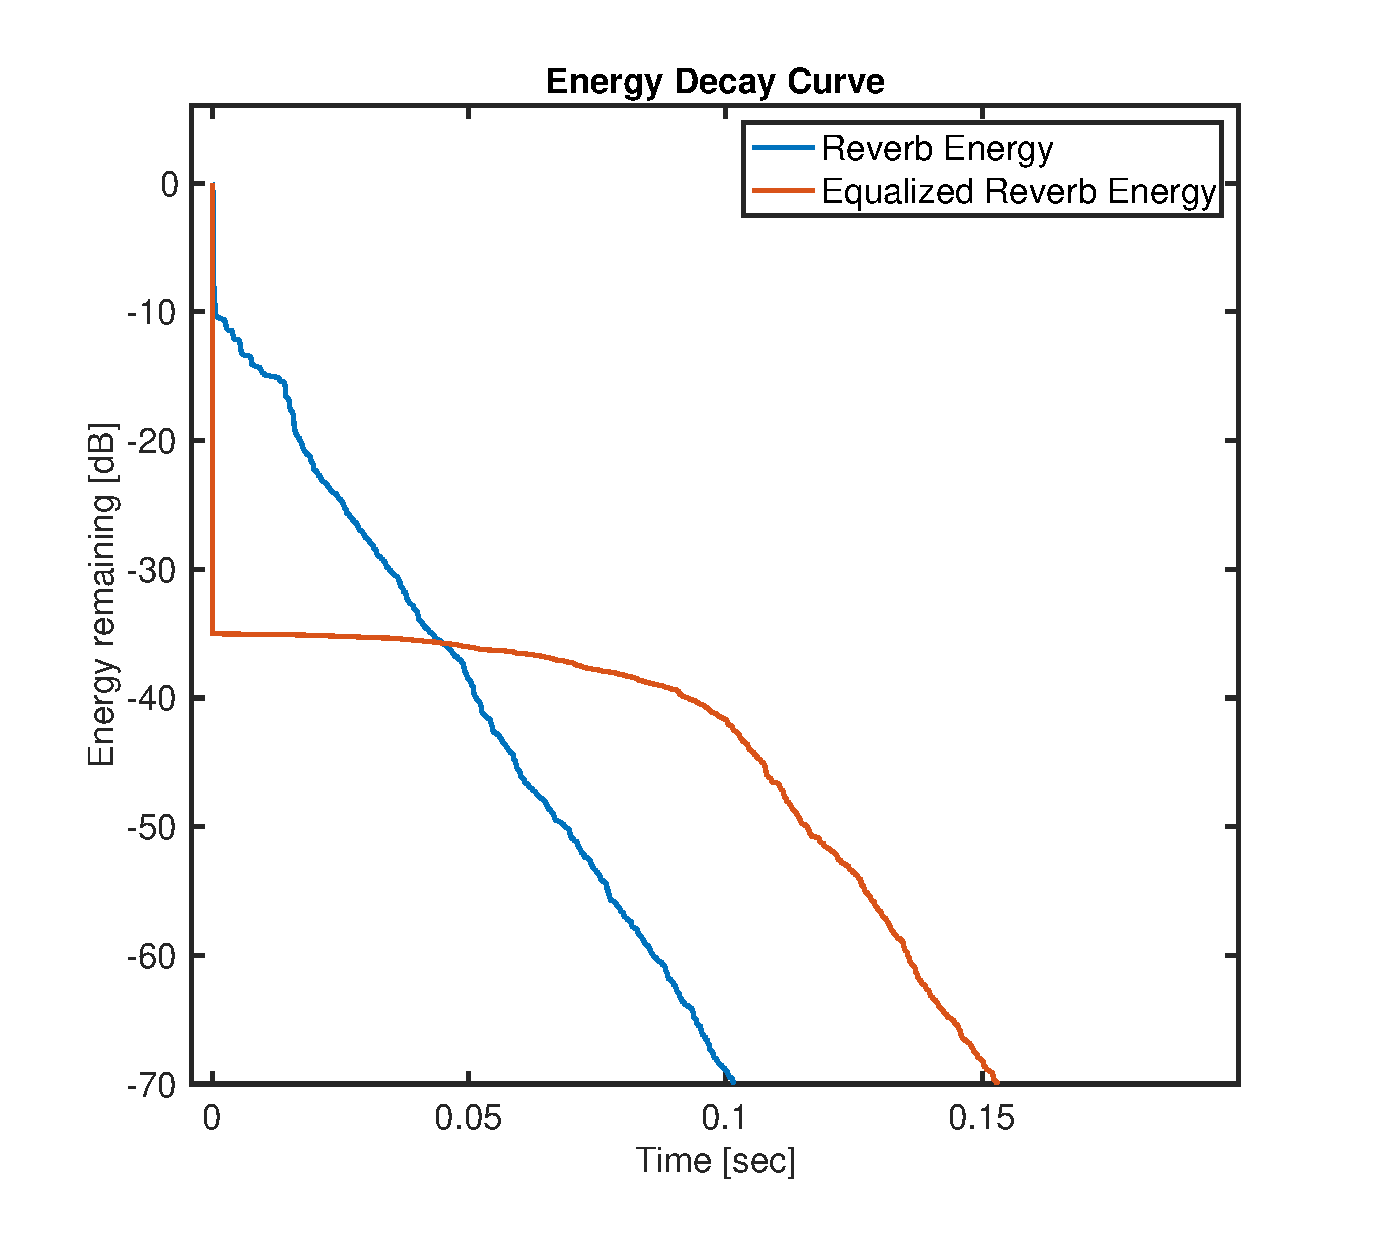
\includegraphics[width=\linewidth]{EDC_0p75N60_div_M_minus_1}
			\end{subfigure}
		\end{minipage}
	}
	% Dummy subfigure for referencing row C
	\refstepcounter{subfigure}
	\label{subfig:params_p2_compare:C}
	
	\vspace{1em}
	
	% ROW D
	\makebox[\textwidth][l]{%
		\begin{minipage}{0.23\textwidth}
			\centering
			\raggedleft{\footnotesize \textbf{(d)} \newline $p_2 = 0.5 \cdot \mathrm{N60}  / (M-1)$} \\
		\end{minipage}%
		\begin{minipage}{0.66\textwidth}
			\begin{subfigure}[t]{0.49\textwidth}
				\centering
				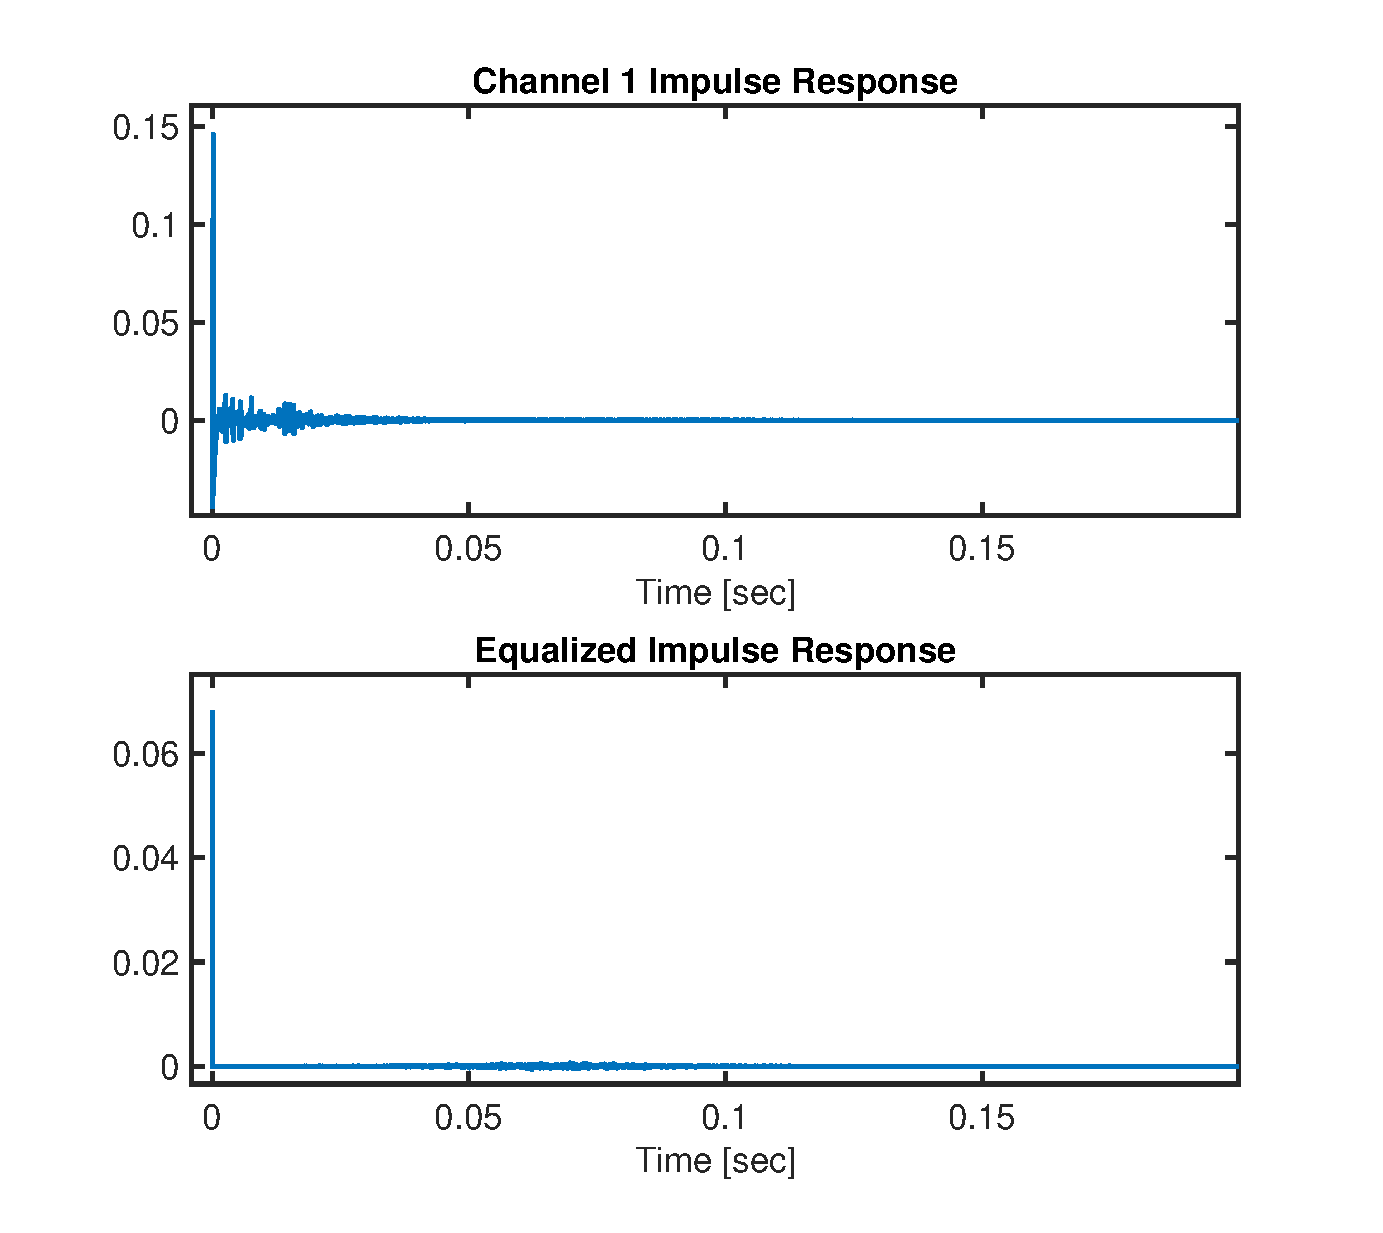
\includegraphics[width=\linewidth]{EIR_0p5N60_div_M_minus_1}
			\end{subfigure}
			\hfill
			\begin{subfigure}[t]{0.49\textwidth}
				\centering
				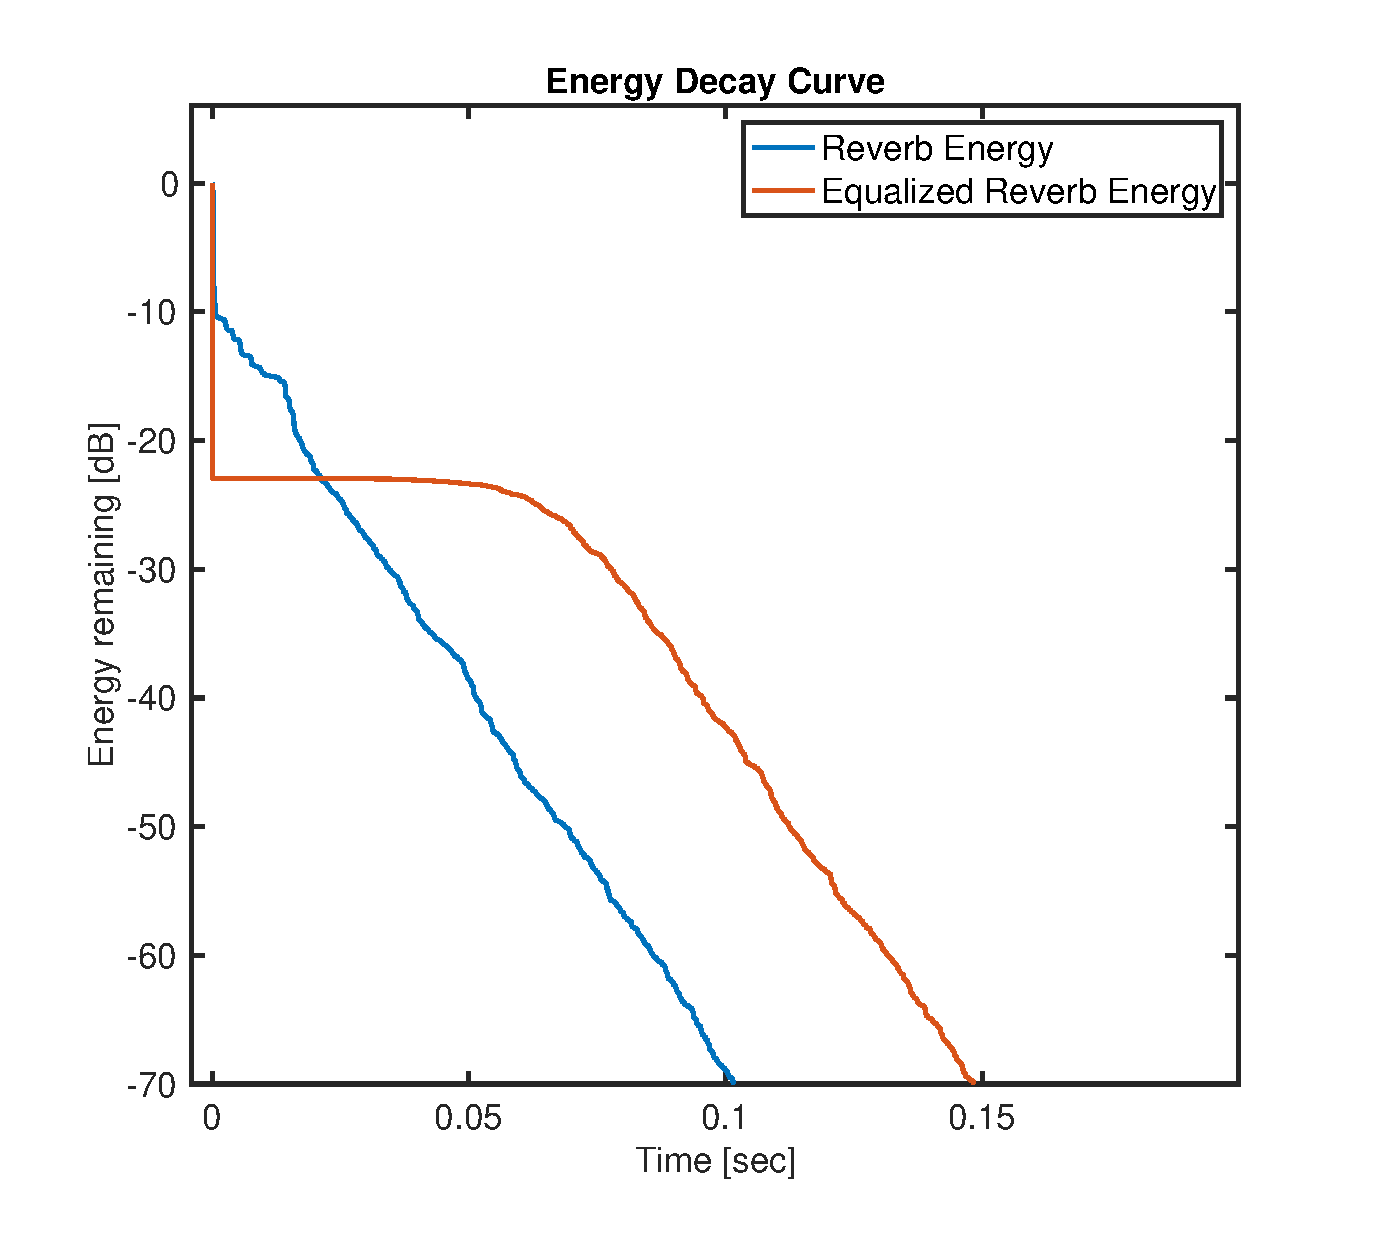
\includegraphics[width=\linewidth]{EDC_0p5N60_div_M_minus_1}
			\end{subfigure}
		\end{minipage}
	}
	% Dummy subfigure for referencing row D
	\refstepcounter{subfigure}
	\label{subfig:params_p2_compare:D}
	
	\caption[Impact of MC-LP order on DAP dereverberation performance]{Impact of MC-LP order ($p_2$) on DAP dereverberation performance. Prediction orders are quantified relative to the actual length of the FIR channel ($L$) and the number of samples corresponding to the T60 of the channel ($\mathrm{N60}$). Figure \ref{fig:params_p2_stage1} shows the common source whitening filter used.}
\label{fig:params_p2_compare}
	
\end{figure}

Accross all test cases, it was noted that reverberation cancellation performance of the inverse filter produced by MC-LP was significantly worse than the MINT inverse filter. While $p_2=L/\left(M-1\right)$ results in \qty{250}{\decibel} of reverberation cancellation in the MINT inverse filter, the MC-LP-estimated inverse filter only acheives approximately \qty{32}{\decibel} cancellation. This makes sense since the MC-LP normal equations (Equation \ref{eq:mc_yule_walker}) are susceptable to numerical error which results in estimation variance. This is especially true for the equalization of the later part of the RIR, where reverberation energy is lower (i.e., the effective SNR of the reverberation is lower). This increase in estimation variance occurs due to the reduced reverberant energy and due to the longer autocorrelation lags involved in the normal equations, for which there is less data available (i.e., there is less overlapping data between the lagged and not-lagged signals). This practical effect of estimating correlation at longer lags is well known and is the motivation for biased estimators such as the windowed autcorrelation estimator used in the periodogram PSD estimate \citep{oppenheim1999discrete}. Additionally, although the source-whitening filter was trained on the clean speech signal, it has its own estimation variance and its performance is also limited by its finite prediction order ($p_1 = 4000$). Any imperfections in the source-whitening will distort the MC-LP results.

Interestingly, reverberation suppression was observed to effectively plateau at around \qty{30}{\decibel} - \qty{35}{\decibel} for $p_2 \ge 0.75 \cdot \mathrm{N60} / \left(M-1\right)$. Essentially, the RIR is near-perfectly equalized almost instantaneously (like the MINT), but towards the end of the reverberation tail, increased estimation variance leads to increasingly worse performance, resulting in reverberation energy increasing again. Beyond the time spanned by the prediction error filter, delay-and-predict has no impact on the RIR, thus the decay rate returns to that which is dictated by the original RIR.

Therefore, it was concluded that it is not possible in practice to acheive the same dereverberation performance as the MINT when using MC-LP-based dereverberation algorithms. For this reason, it does not make sense to choose $p_2$ based on the MINT conditions for perfect equalization, but rather based on the practical boundaries resulting from numerical limitations. Figure \ref{fig:params_p2_compare} suggests that setting $p_2$ greater than approximately $0.75 \cdot \mathrm{N60} / \left(M-1)\right)$ is reasonable. In practice, the $N60$ is unknown, so the MC-LP prediction order should be set as high as is computationally acceptable to sufficiently cancel the longest T60s possible.

\section{Source Whitening Linear Prediction Order} \label{section:params_p1} 

To evaluate the impact of the source-whitening prediction order ($p_1$), the MC-LP order was fixed at $p_2 = \mathrm{N60} / \left(M-1\right)$, and $p_1$ was varied. The same sample rate, source signal/length, and four-channel RIR from the last section was used. The source-whitening prediction order $p_1=200$ was evaluated first to match the original configuration of \cite{triki2006delay} (scaled by sample rate from \qty{8}{\kilo\hertz} to \qty{16}{\kilo\hertz}). Next, $p_1 = p_2 \cdot \left(M-1\right)$ was evaluated to match the spectral resolution of the source-whitening stage to the effective spectral resolution of the MC-LP stage. Since the MINT dictates that a length-$L$ RIR can be perfectly equalized using $M$ channels with $M$ corresponding length $\left(p_2+1\right) = \left(L-1\right)/\left(M-1\right)$ equalizer filters, it can be said that the effective spectral resolution of MINT equalizer (and therefore any multichannel filter-and-sum equalizer) is that of a FIR filter of length $L= \left(p_2+1\right) \cdot \left(M-1\right)  + 1 \approx p_2 \cdot \left(M-1\right)$. Therefore setting $p_1 = p_2 \cdot (M-1)$ effectively matches the spectral resolution of the source-whitening stage to the MC-LP stage as previously stated. Figure \ref{fig:params_p1_compare} shows the EIR and EDC performance for each case. For more detailed plots of the inner-workings of the algorithm in this evaluation, refer to Appendix \ref{section:appendix:params_p1}.


% Test Conditions:
% - Source Signal = SA1.WAV
% - Source length = 348366
% - RIR = MYRiAD SAL Measured RIR (T60 = 2100 msec, Truncated Exponentially to T60 = 100 msec)
% - RIR length = 3200
% - T60 = 100 msec (N60 = 1600 samples)
% - SNR = 300 dB
% - Noise Signal = office ventilation
% - SIR = Inf dB
% - Interference Signal = None
%
% Delay-and-Predict config:
% - Number of Microphones (M) = 4
% - Source whitening order (p1) = varied
% - Multichannel Linear Prediction order (p2) = 533 (N60 / (M-1))
% - Source whitening Enabled? = 1
% - Source whitening on clean speech? = 1

\begin{figure}[H]
	\centering
	
	% ROW A
	\makebox[\textwidth][l]{%
		\begin{minipage}{0.23\textwidth}
			\centering
			\raggedleft{\footnotesize \textbf{(a)} \newline $p_1 = 200$ \newline \citep{triki2006delay}} \\
		\end{minipage}%
		\begin{minipage}{0.66\textwidth}
			\begin{subfigure}[t]{0.49\textwidth}
				\centering
				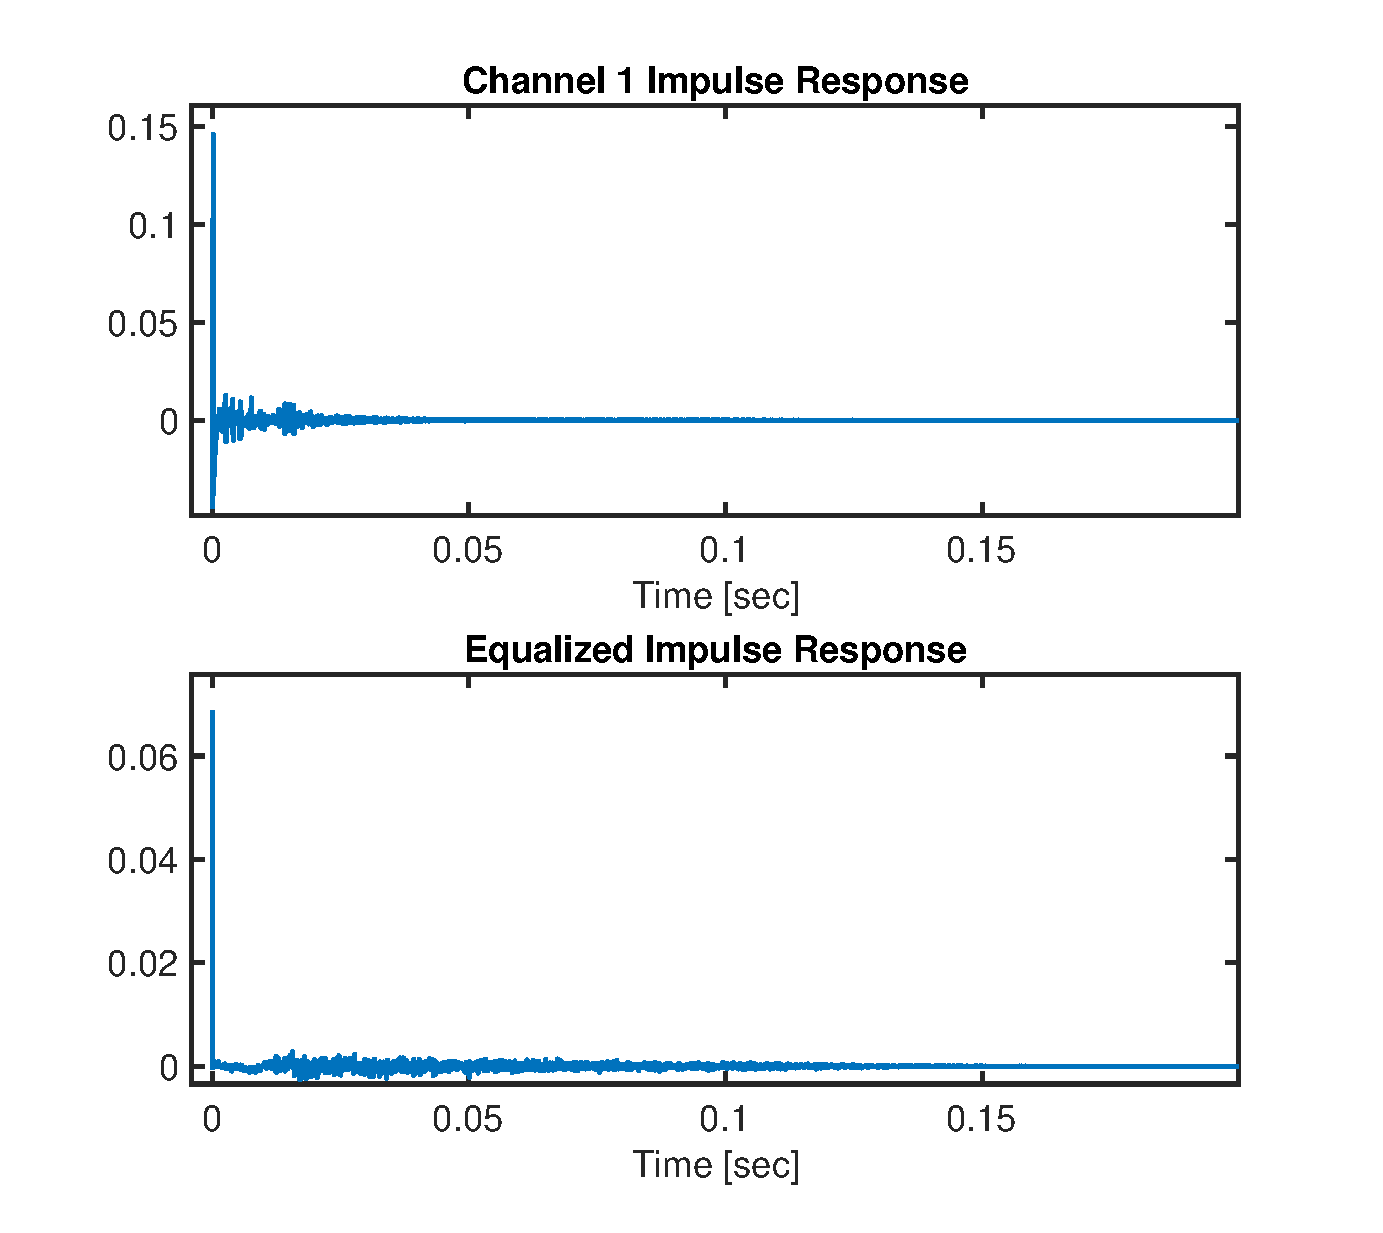
\includegraphics[width=\linewidth]{EIR_p1_200}
			\end{subfigure}
			\hfill
			\begin{subfigure}[t]{0.49\textwidth}
				\centering
				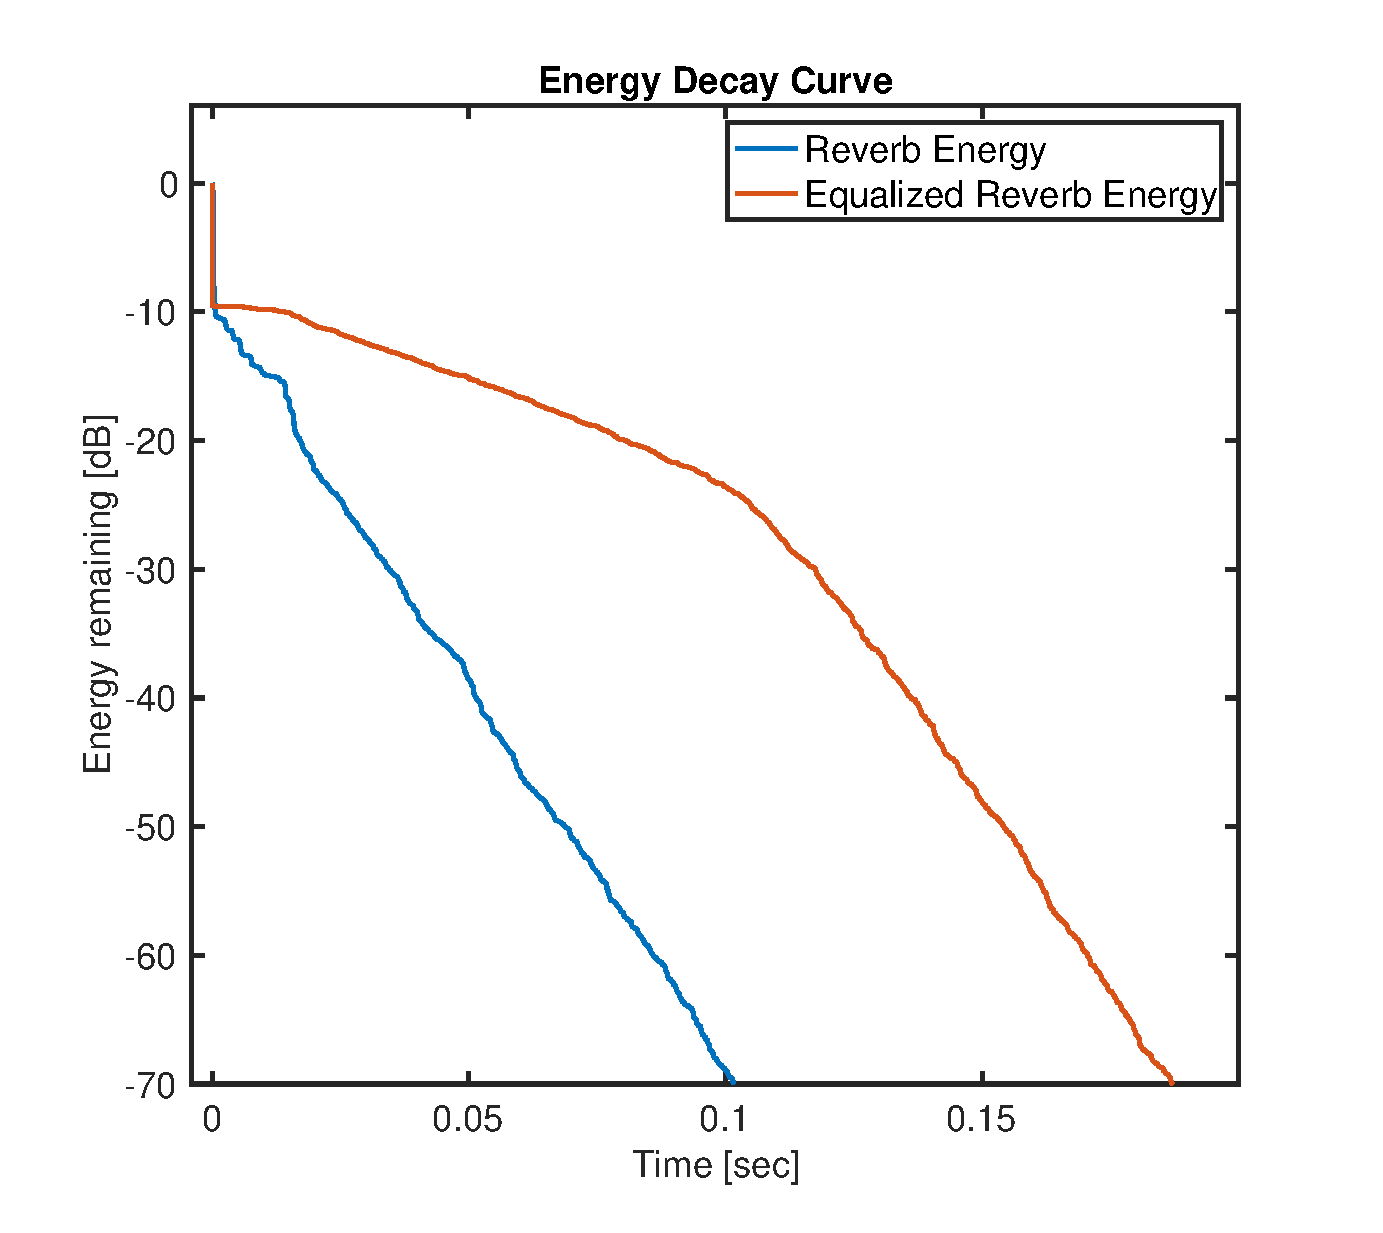
\includegraphics[width=\linewidth]{EDC_p1_200}
			\end{subfigure}
		\end{minipage}
	}
	% Dummy subfigure for referencing row A
	\refstepcounter{subfigure}
	\label{subfig:params_p1_compare:A}
	
	\vspace{1em}
	
	% ROW B
	\makebox[\textwidth][l]{%
		\begin{minipage}{0.23\textwidth}
			\centering
			\raggedleft{\footnotesize \textbf{(b)} \newline $p_1 = 1000$} \\
		\end{minipage}%
		\begin{minipage}{0.66\textwidth}
			\begin{subfigure}[t]{0.49\textwidth}
				\centering
				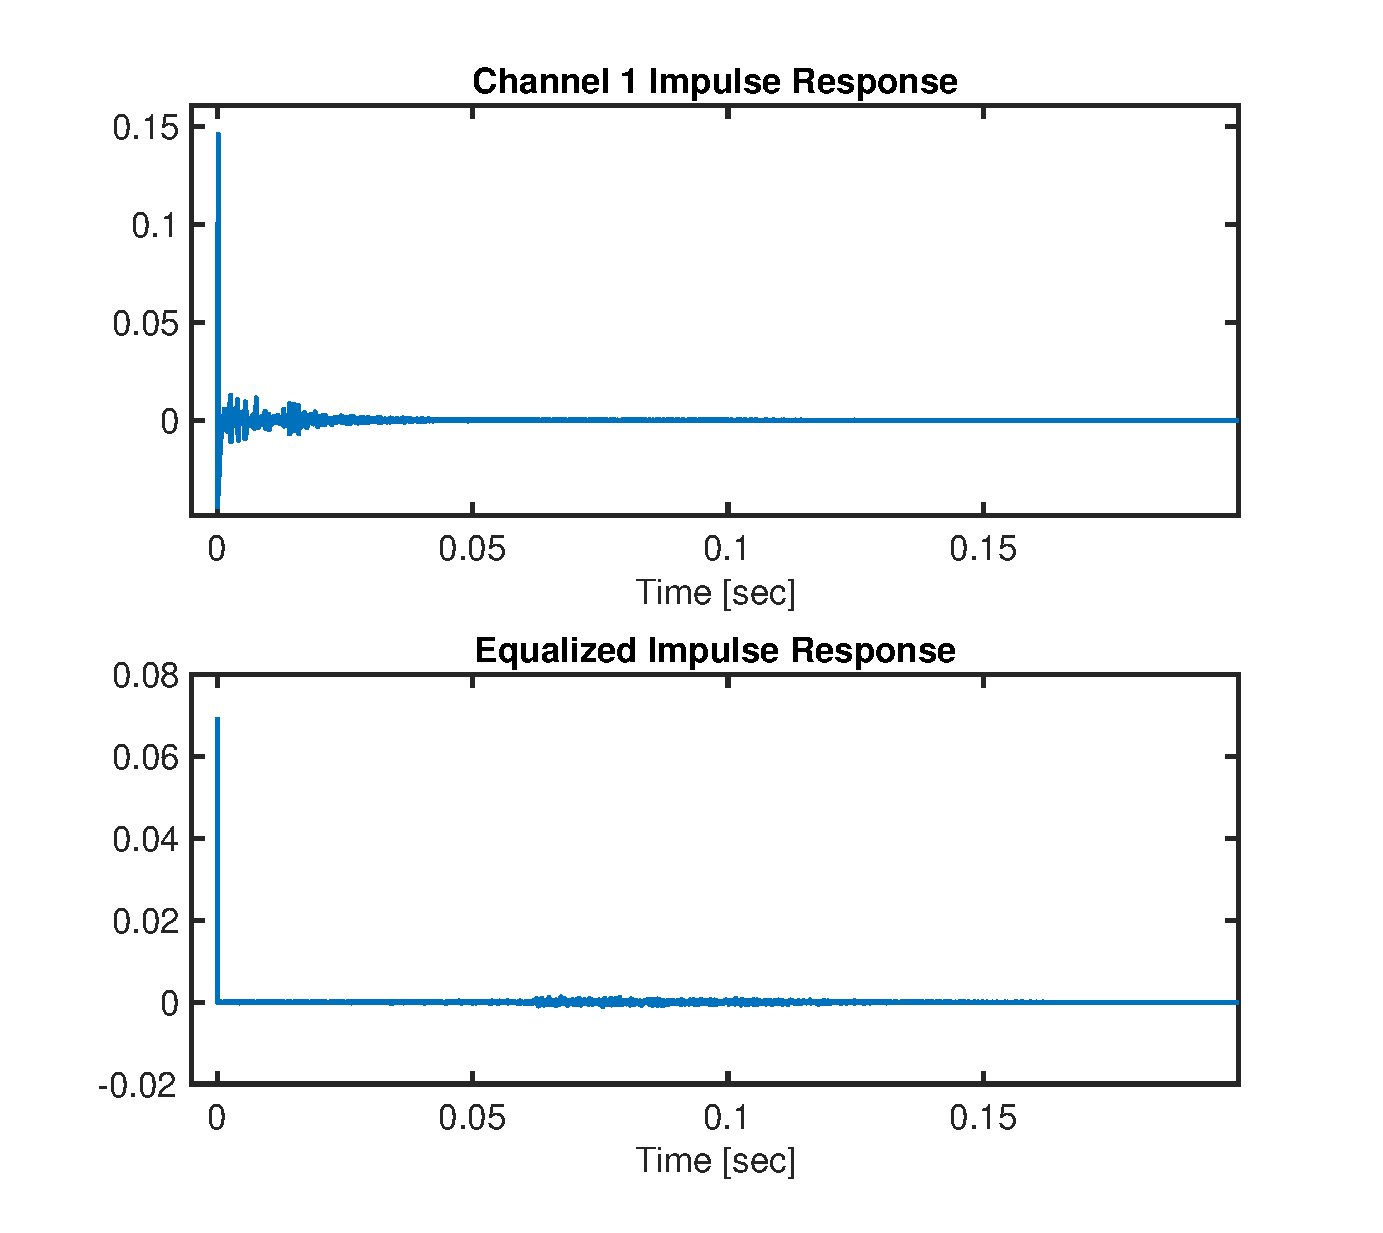
\includegraphics[width=\linewidth]{EIR_p1_1000}
			\end{subfigure}
			\hfill
			\begin{subfigure}[t]{0.49\textwidth}
				\centering
				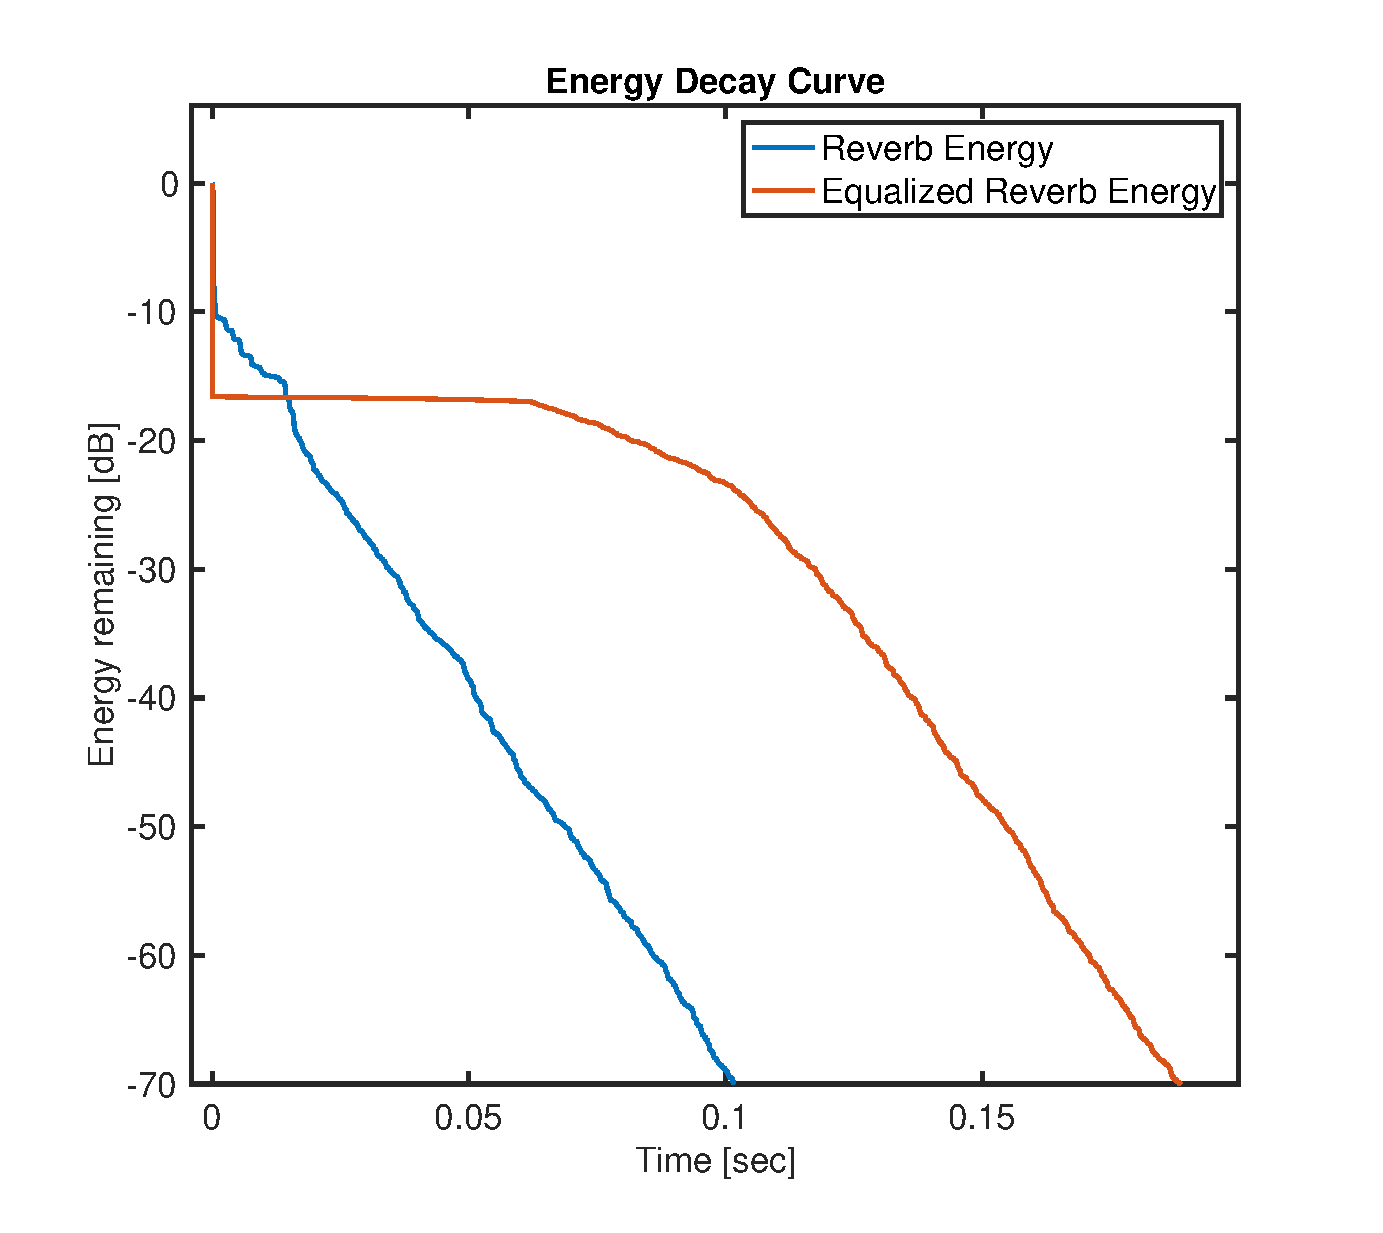
\includegraphics[width=\linewidth]{EDC_p1_1000}
			\end{subfigure}
		\end{minipage}
	}
	% Dummy subfigure for referencing row B
	\refstepcounter{subfigure}
	\label{subfig:params_p1_compare:B}
	
	\vspace{1em}
	
	% ROW C
	\makebox[\textwidth][l]{%
		\begin{minipage}{0.23\textwidth}
			\centering
			\raggedleft{\footnotesize \textbf{(c)} \newline $p_1 = 1600$ \newline ($p_1 = p_2 \cdot \left(M-1\right)$)} \\
		\end{minipage}%
		\begin{minipage}{0.66\textwidth}
			\begin{subfigure}[t]{0.49\textwidth}
				\centering
				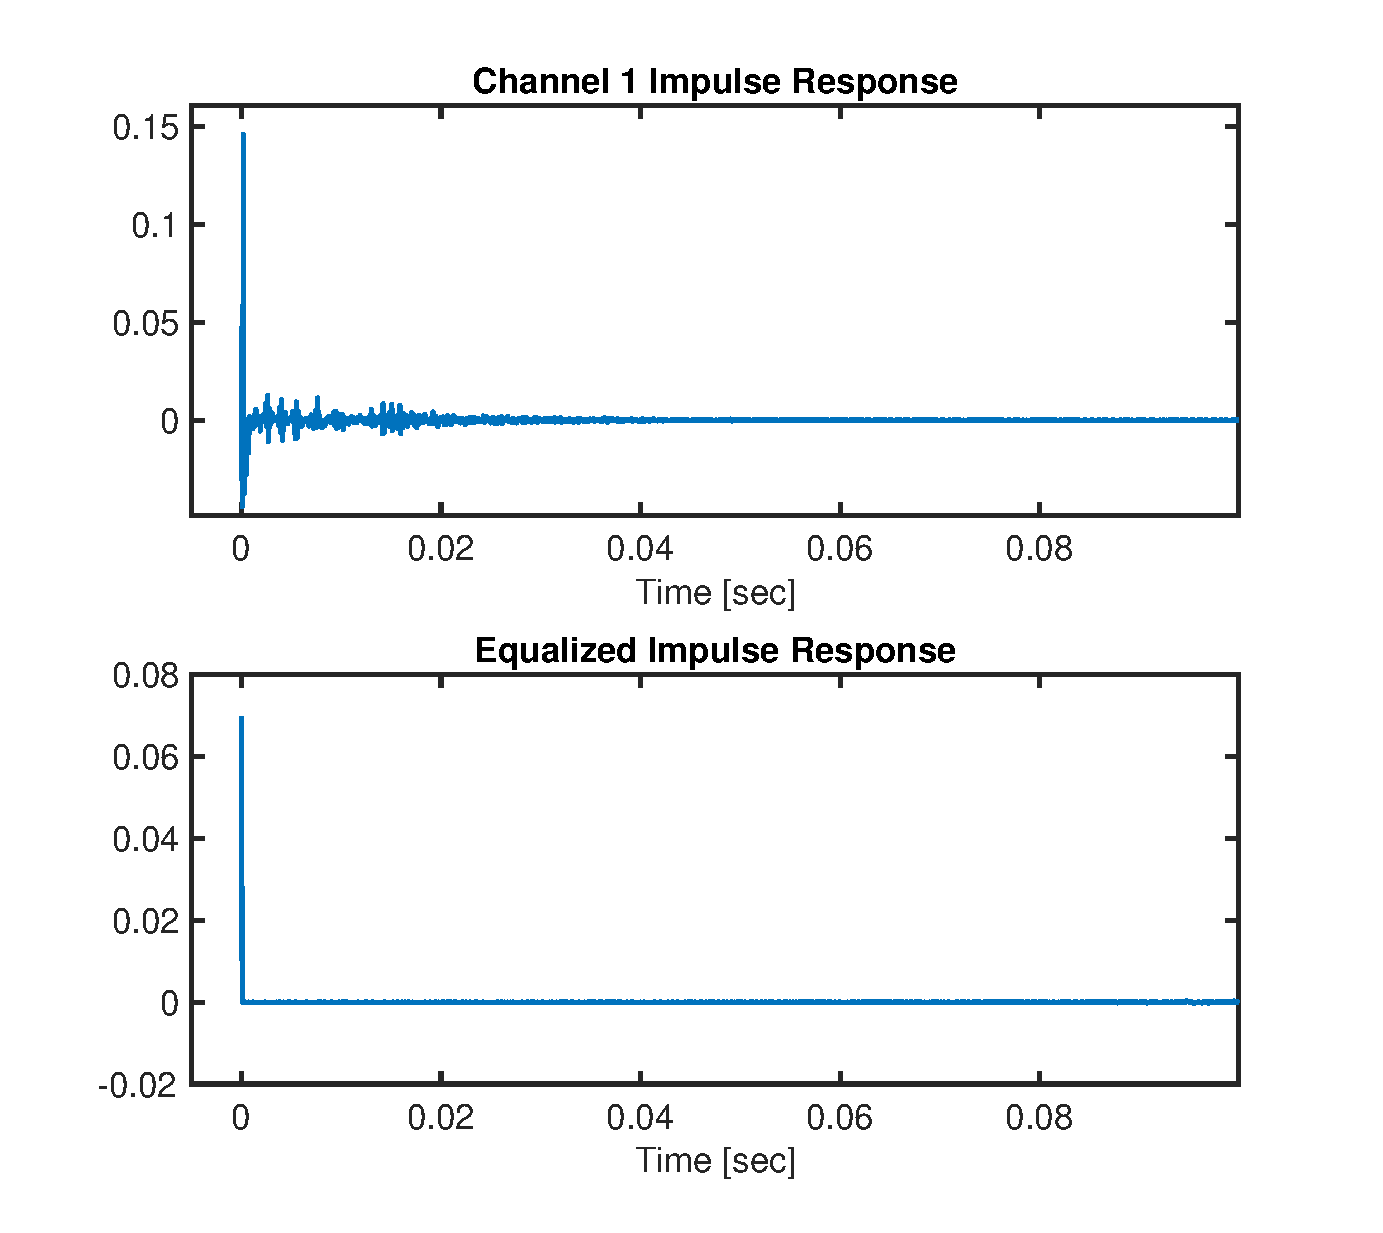
\includegraphics[width=\linewidth]{EIR_p1_based_on_p2}
			\end{subfigure}
			\hfill
			\begin{subfigure}[t]{0.49\textwidth}
				\centering
				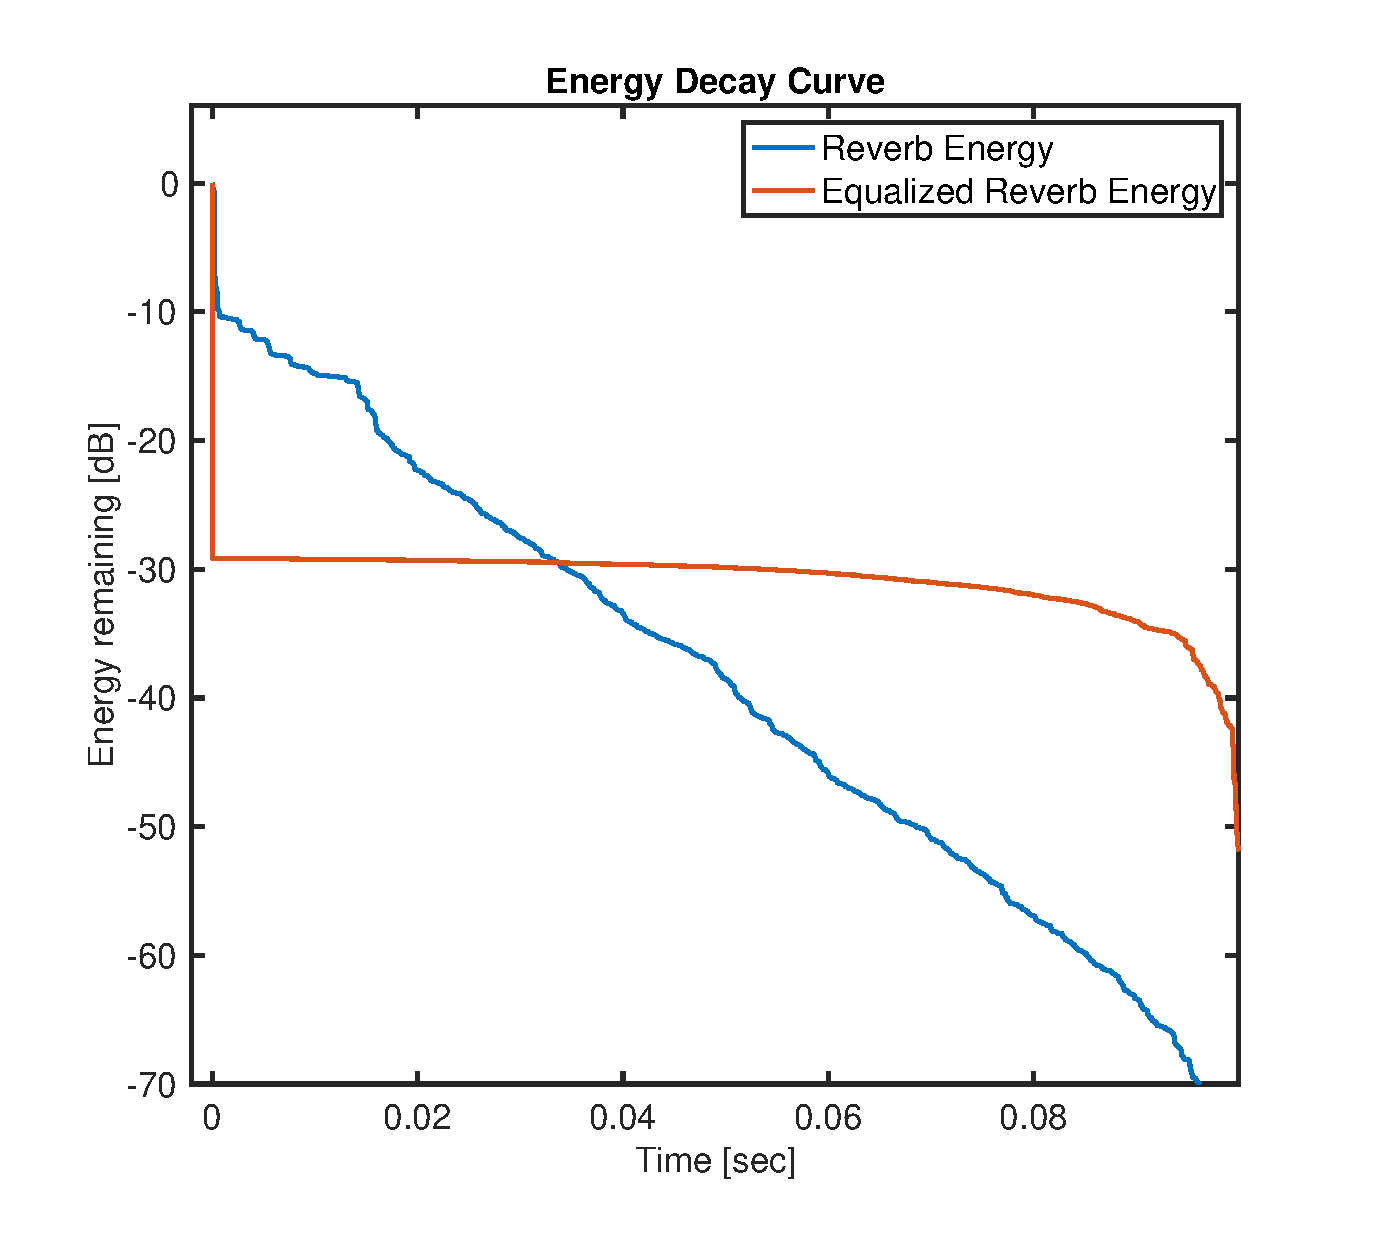
\includegraphics[width=\linewidth]{EDC_p1_based_on_p2}
			\end{subfigure}
		\end{minipage}
	}
	% Dummy subfigure for referencing row C
	\refstepcounter{subfigure}
	\label{subfig:params_p1_compare:C}
	
	\vspace{1em}
	
	% ROW D
	\makebox[\textwidth][l]{%
		\begin{minipage}{0.23\textwidth}
			\centering
			\raggedleft{\footnotesize \textbf{(d)} \newline $p_1 = 3200$ \newline ($p_1 = 2 \cdot p_2 \cdot \left(M-1\right)$)} \\
		\end{minipage}%
		\begin{minipage}{0.66\textwidth}
			\begin{subfigure}[t]{0.49\textwidth}
				\centering
				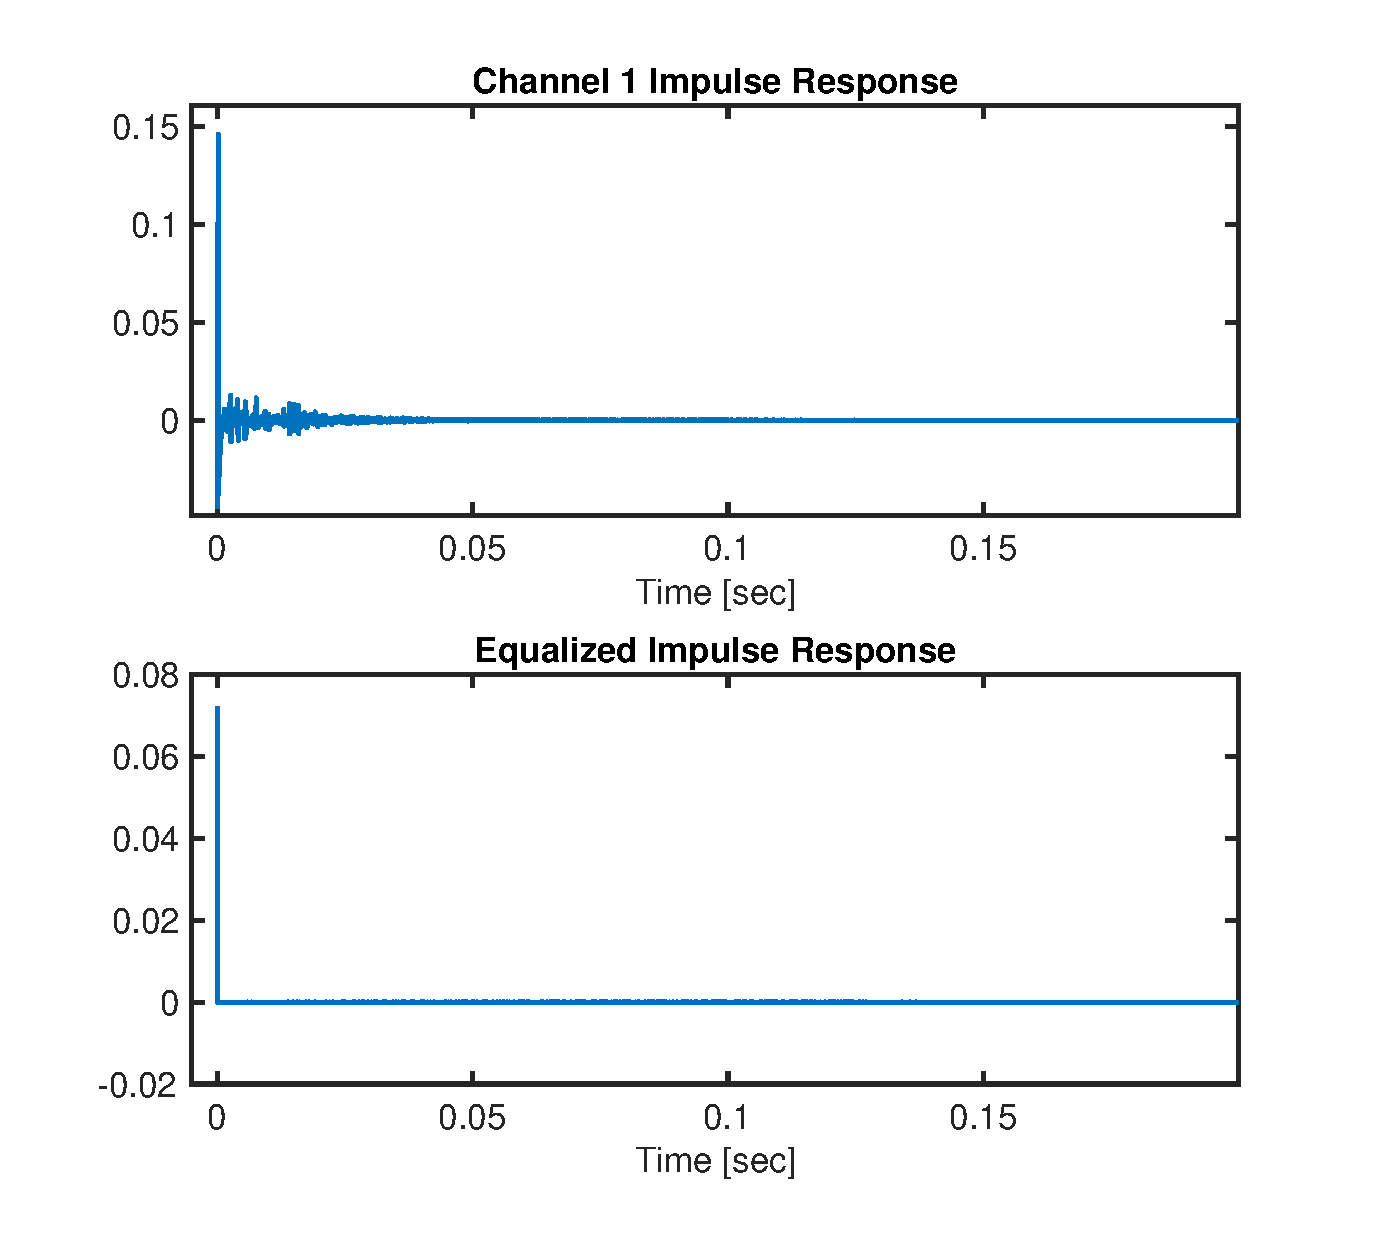
\includegraphics[width=\linewidth]{EIR_p1_2x_p2}
			\end{subfigure}
			\hfill
			\begin{subfigure}[t]{0.49\textwidth}
				\centering
				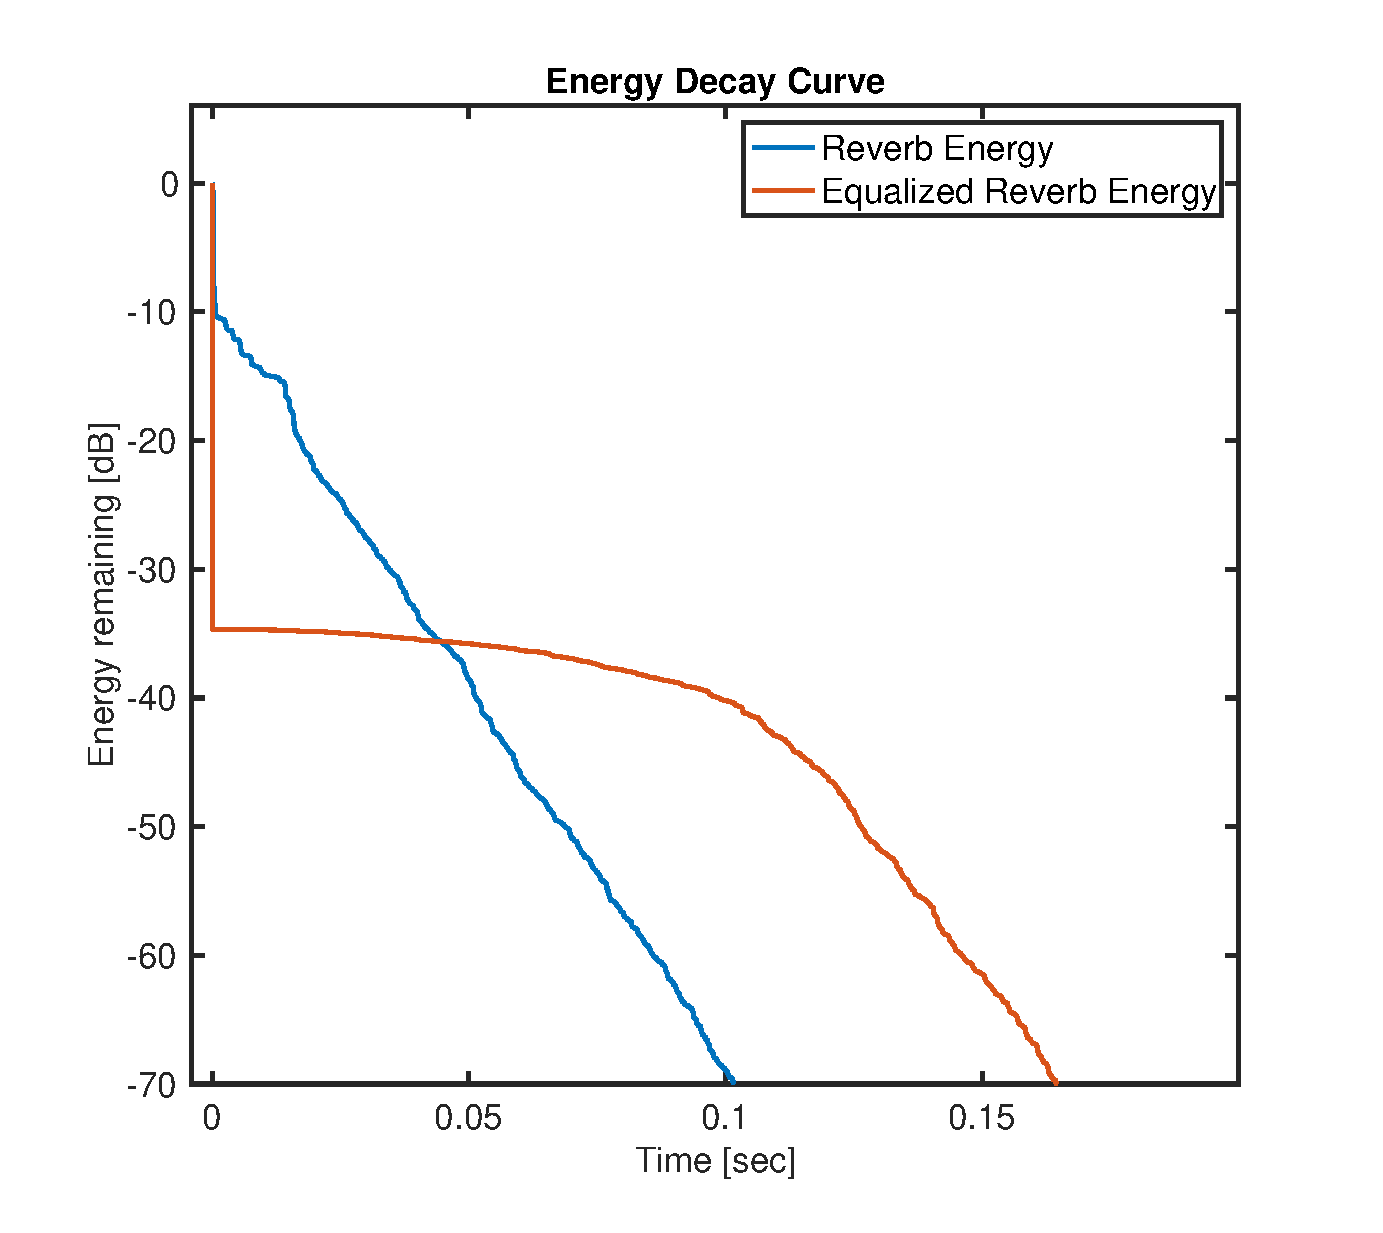
\includegraphics[width=\linewidth]{EDC_p1_2x_p2}
			\end{subfigure}
		\end{minipage}
	}
	% Dummy subfigure for referencing row D
	\refstepcounter{subfigure}
	\label{subfig:params_p1_compare:D}
	
	\caption[Impact of source-whitening prediction order on DAP dereverberation performance]{Impact of source-whitening prediction order ($p_1$) on DAP dereverberation performance. Prediction orders are quantified relative to the MC-LP order, which was set to $\mathrm{p_2} = \mathrm{N60} / \left(M-1\right)$}
	\label{fig:params_p1_compare}
	
\end{figure}

It was noted that the algorithm provides very little reverberation cancellation for low source-whitening prediction orders, and that reverberation attenuation plateaus around \qty{35}{\decibel} when the source-whitening prediction order rises above approximately $p_1 = 1.25 \cdot p_2 \cdot (\left(M-1\right)$. This demonstrates the importance of selecting a source-whitening prediction order such that that its spectral resolution matches or exceeds the effective spectral resolution of the MC-LP stage. This makes intuitive sense since any AR characteristics of the source that are visible within the spectral resolution the MC-LP analysis which have not been removed by the source-whitening stage, will be captured in the MC-LP analysis and thus will distort the estimate of the true system inverse.

\section{Blind Deconvolution Performance}

To analyze the behaviour of the full blind dereverberation algorithm (i.e., blindly estimating the source AR properties), a single test condition was used to compare the performance of the MINT equalizer, the DAP equalizer generated using a source-whitening filter trained on clean speech (i.e., the supervised DAP equalizer), and the blind DAP equalizer. The source signal used was a \qty{60}{\sec} sample from the TMIT database and the four-channel RIR was the ``SAL" room from the MYRiAD database, exponentially windowed to a T60 of \qty{1}{\sec}. The MC-LP order was set to $p_2 = 1.25 \cdot N60 / \left(M-1\right)=6667$ and the source-whitening prediction order was set to $p_1 = 1.25 \cdot p_2 \cdot \left(M-1\right)=25001$. The spectrogram plots were generated using a different speech signal from the one used in training. This was done to emphasize the potential that the ``over-whitening" of the training source signal may lead to an added reverberant effect when the equalizer is applied to a different signal (as described in Section \ref{section_dap}). The results for the the MINT, supervised DAP and DAP equalizers are shown in Figure \ref{fig:fullExample_MINT}, Figure \ref{fig:fullExample_NotBlind} and Figure \ref{fig:fullExample_Blind} respectively.

% Test Conditions:
% - Source Signal = TMIT_MKLS0.WAV
% - Source length = 960000
% - RIR = MYRiAD SAL Measured RIR (T60 = 2100 msec, Truncated Exponentially to T60 = 1000 msec)
% - RIR length = 32000
% - T60 = 1000 msec (N60 = 16000 samples)
% - SNR = 300 dB
% - Noise Signal = office ventilation
% - SIR = Inf dB 
% - Interference Signal = None
%
% Delay-and-Predict config:
% - Number of Microphones (M) = 4
% - Source whitening order (p1) = 25001 (1.25 * p2 * (M-1))
% - Multichannel Linear Prediction order (p2) = 6667 (1.25 * N60 / (M-1))
% - Source whitening Enabled? = 1
% - Source whitening on clean speech? = varied

\begin{figure}[H]
	\centering
	\begin{subfigure}[b]{0.38\textwidth}
		\centering
		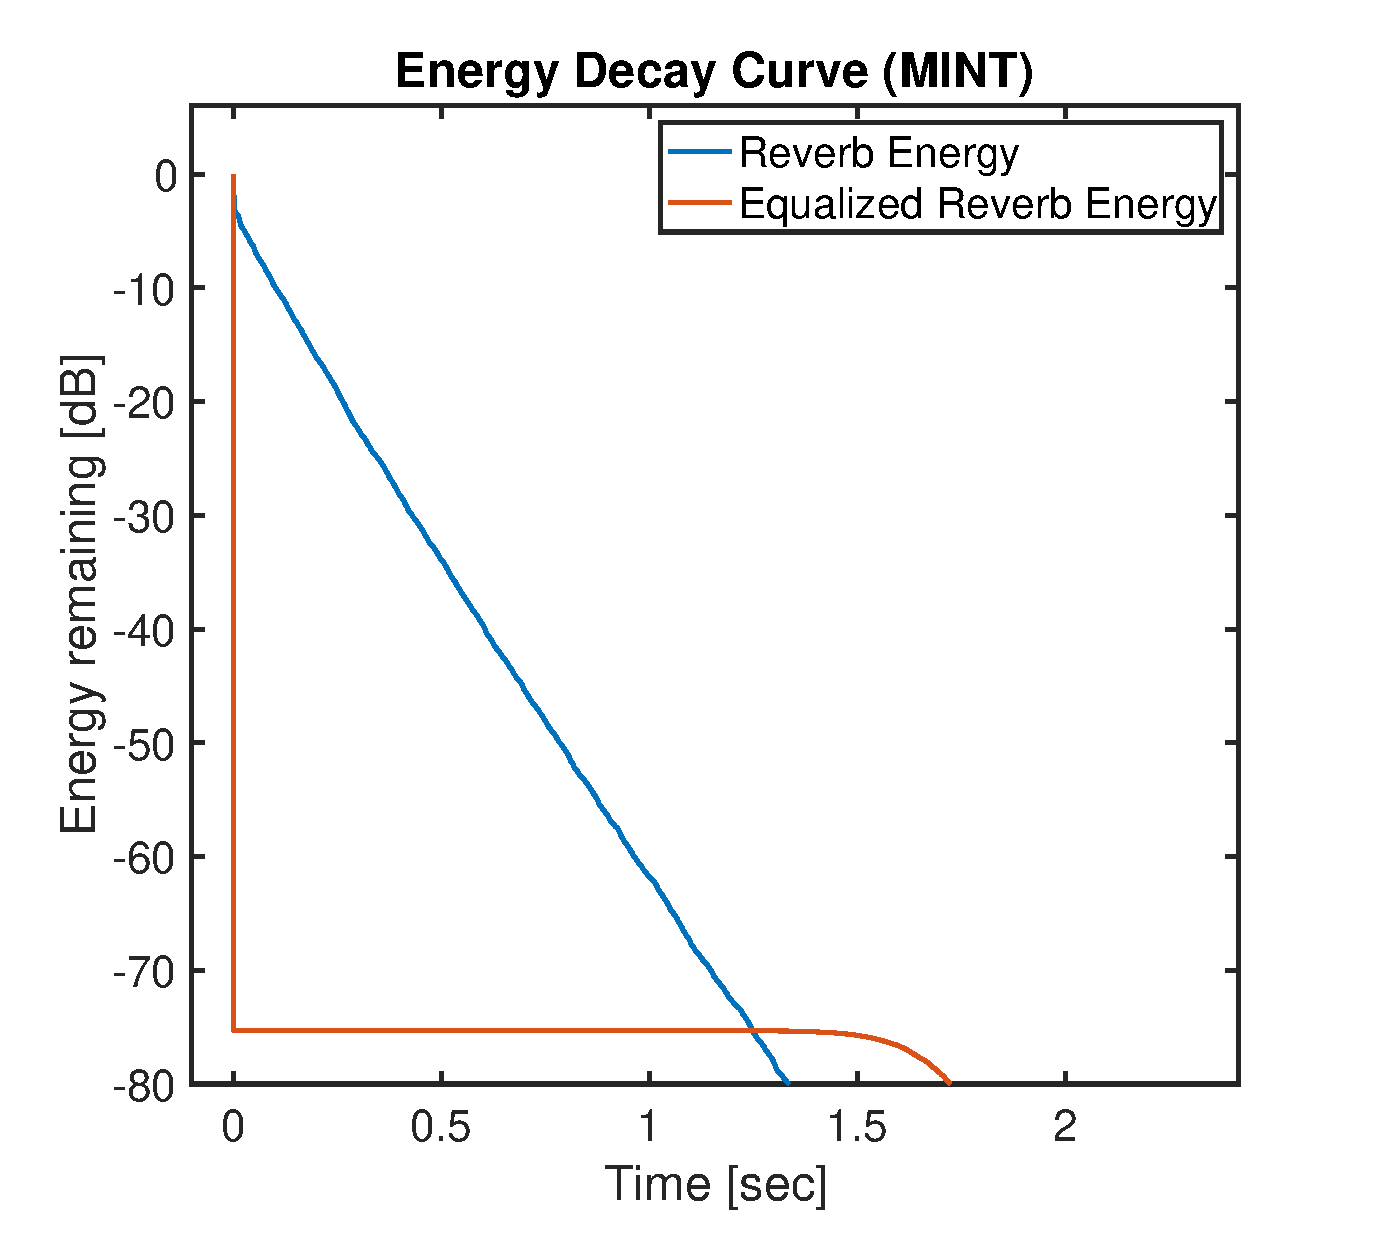
\includegraphics[width=\textwidth]{FullExample_MINT_EDC}
	\end{subfigure}
	\begin{subfigure}[b]{0.49\textwidth}
		\centering
		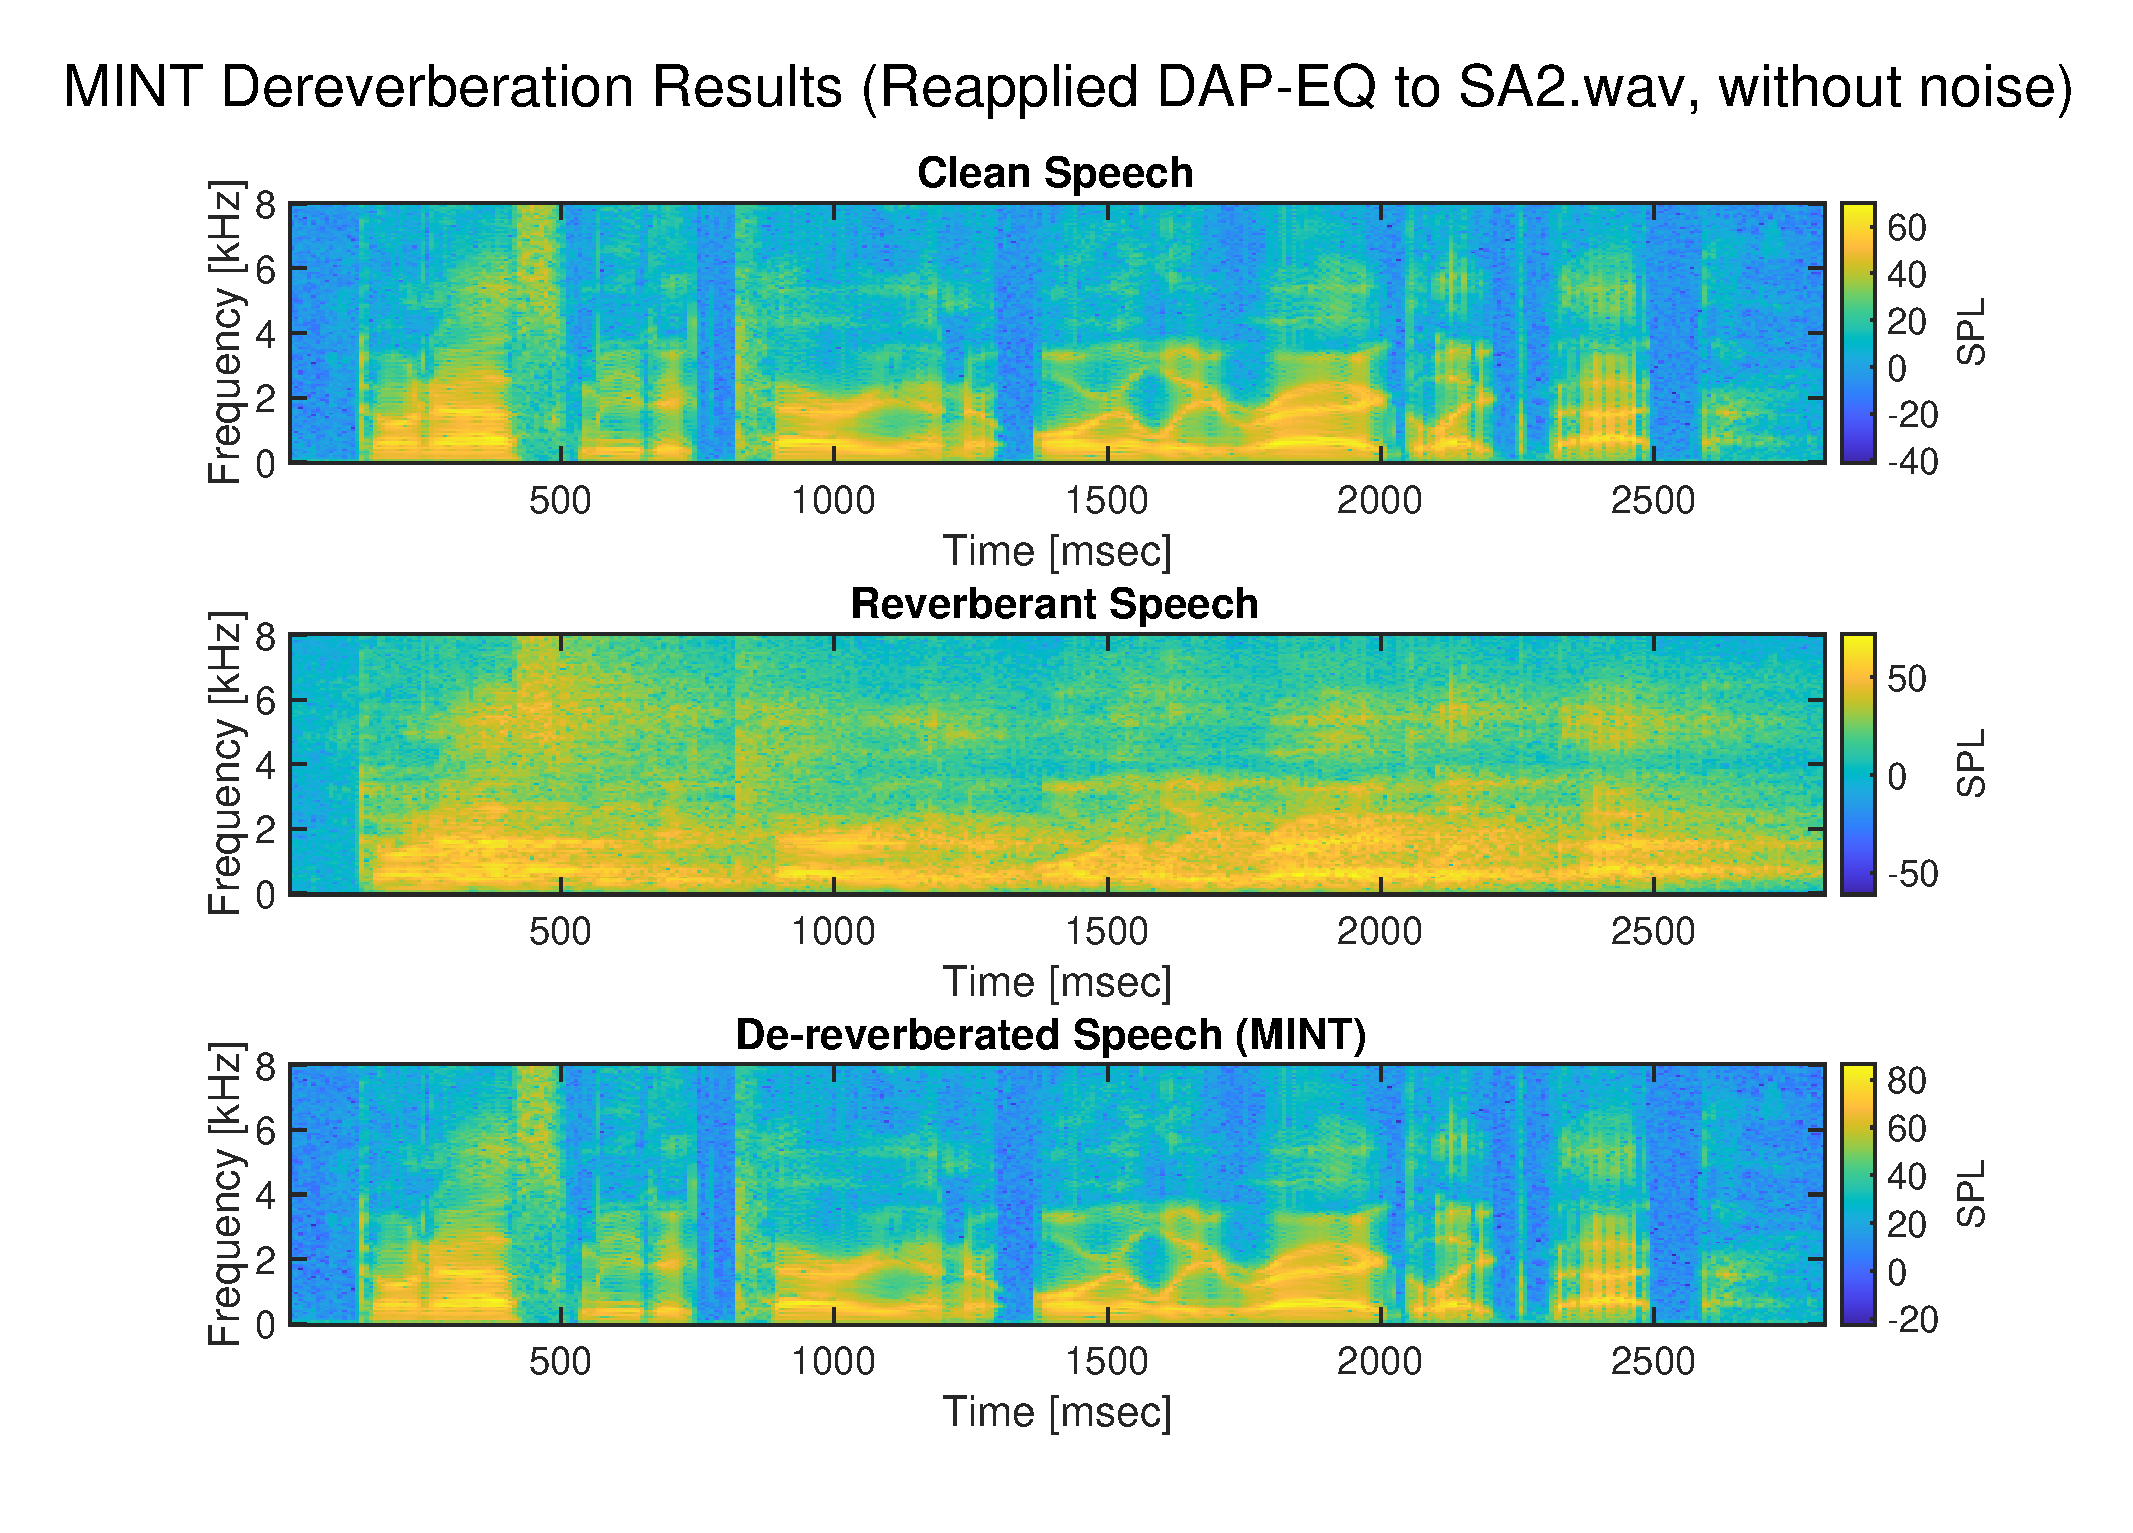
\includegraphics[width=\textwidth]{FullExample_MINT_Spectrogram}
	\end{subfigure}
	\caption[MINT equalizer performance (EDC and spectrogram)]{MINT Equalizer performance (EDC and Spectrogram)}
	\label{fig:fullExample_MINT}
\end{figure}


\begin{figure}[H]
	\centering
	\begin{subfigure}[b]{0.38\textwidth}
		\centering
		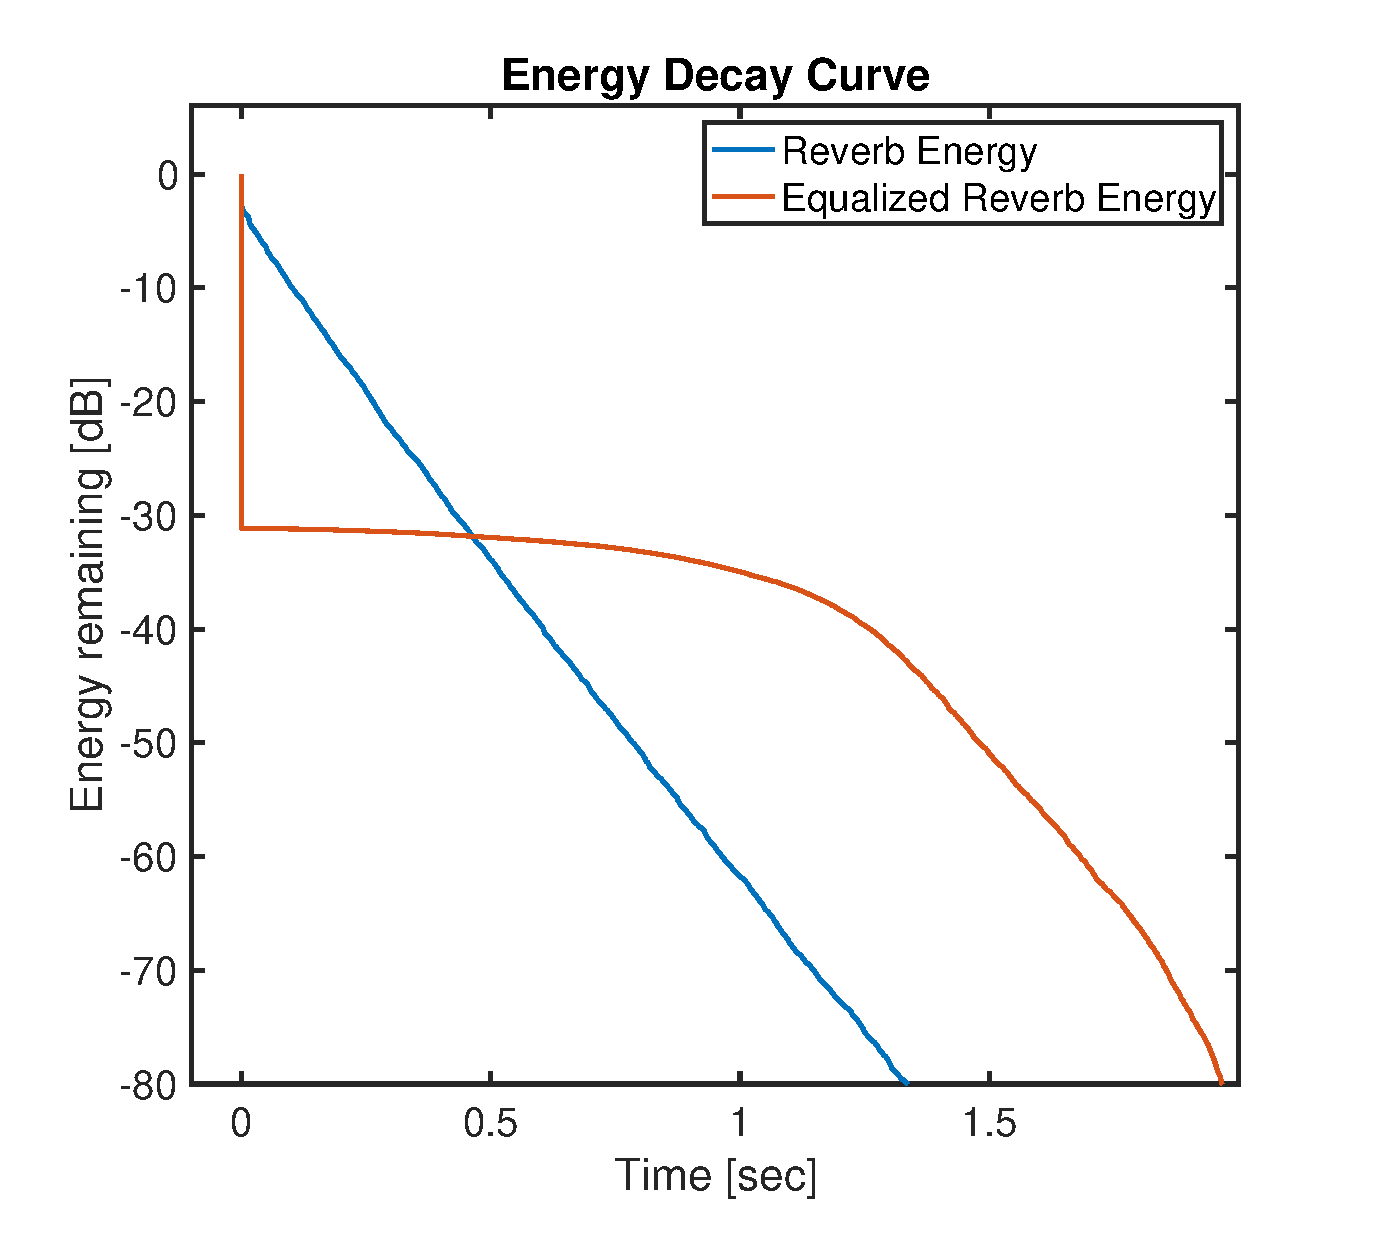
\includegraphics[width=\textwidth]{FullExample_NotBlind_EDC}
	\end{subfigure}
	\begin{subfigure}[b]{0.49\textwidth}
		\centering
		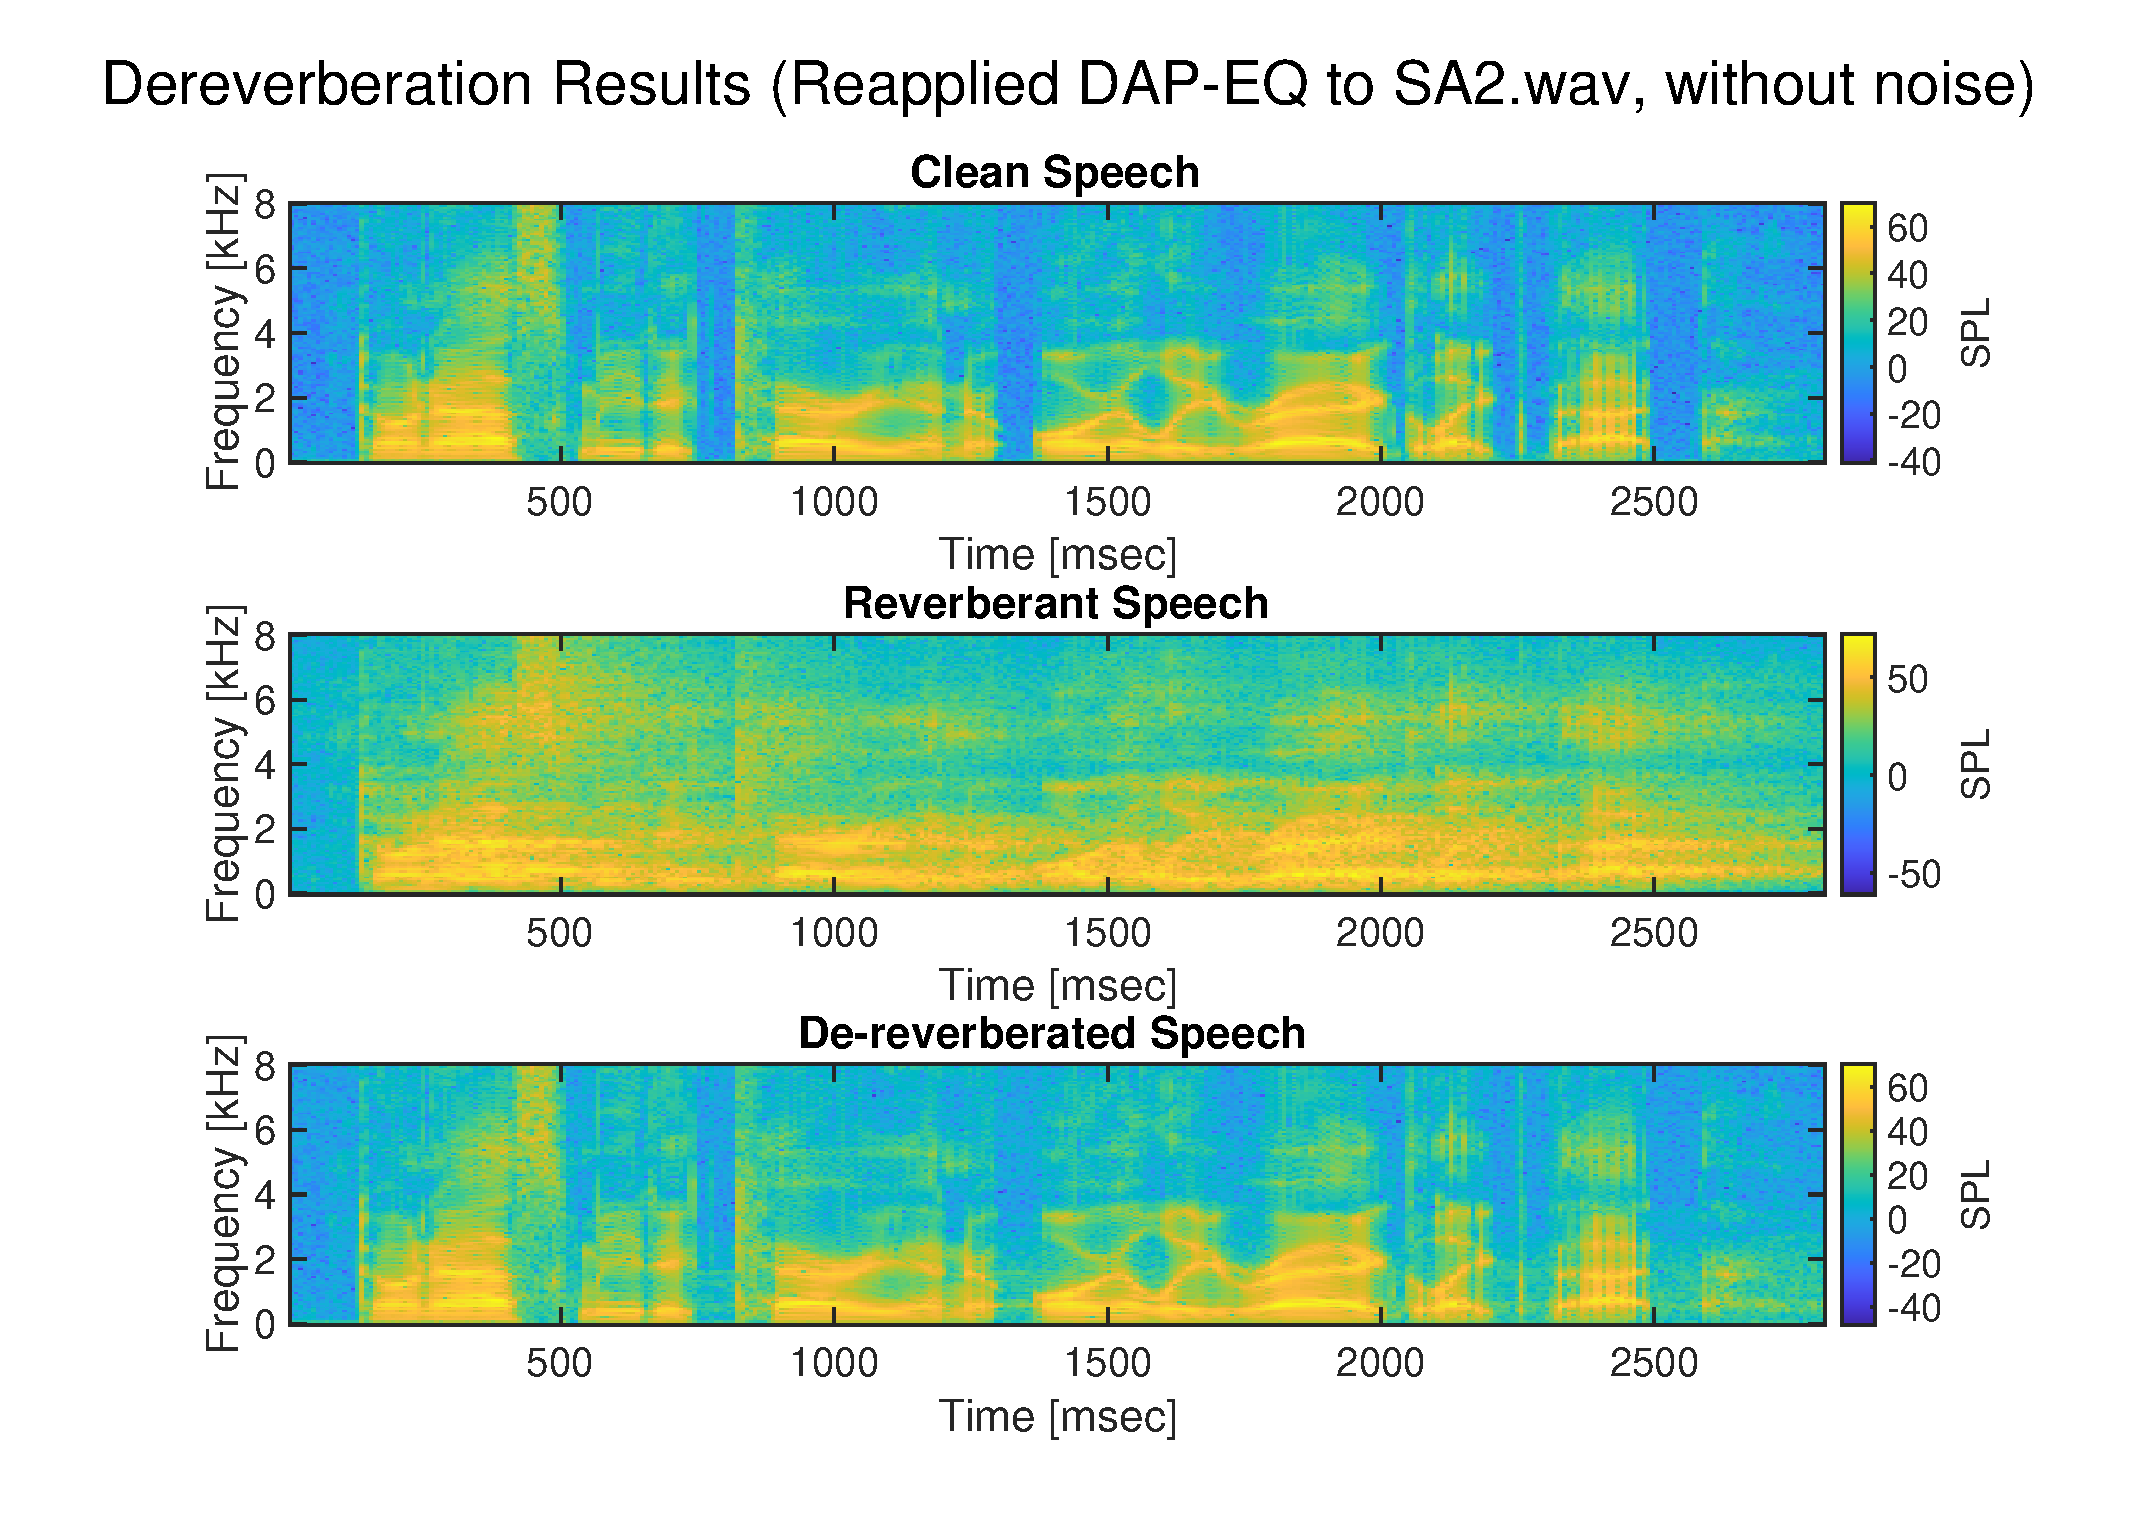
\includegraphics[width=\textwidth]{FullExample_NotBlind_Spectrogram}
	\end{subfigure}
	\caption[Supervised DAP equalizer performance (EDC and spectrogram)]{DAP Equalizer performance (EDC and Spectrogram) with the source-whitening filter computed using clean speech (i.e., not blind)}
	\label{fig:fullExample_NotBlind}
\end{figure}


\begin{figure}[H]
	\centering
	\begin{subfigure}[b]{0.38\textwidth}
		\centering
		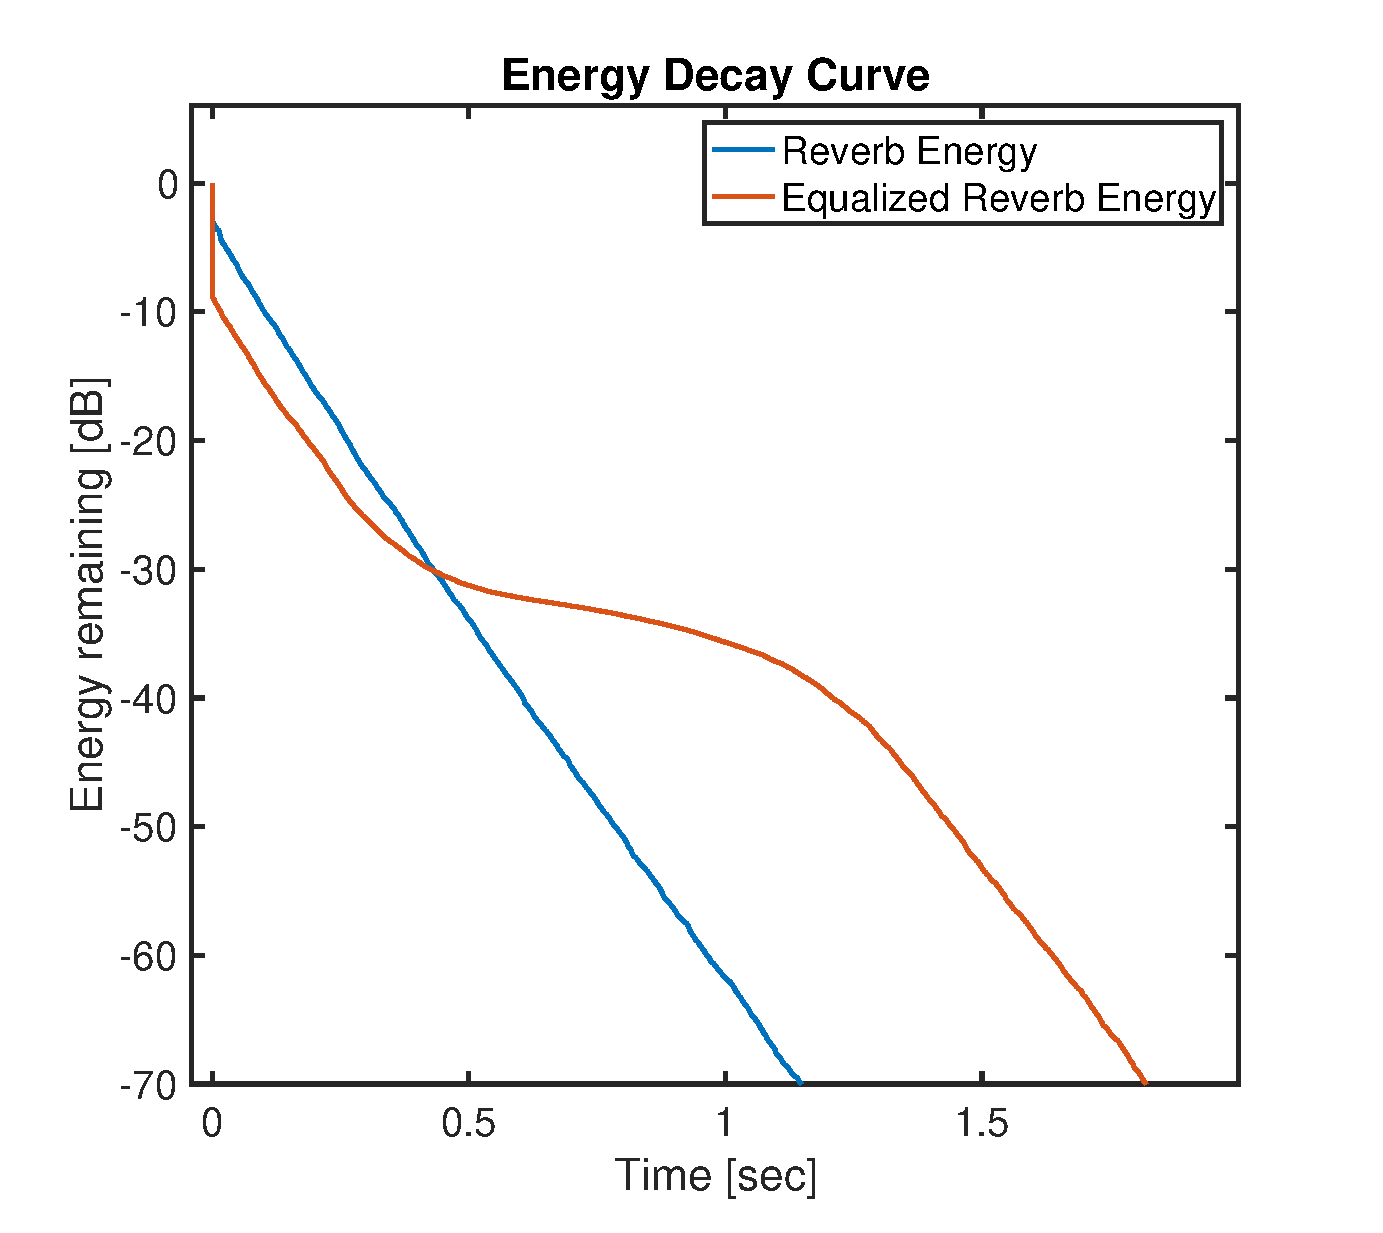
\includegraphics[width=\textwidth]{FullExample_Blind_EDC}
	\end{subfigure}
	\begin{subfigure}[b]{0.49\textwidth}
		\centering
		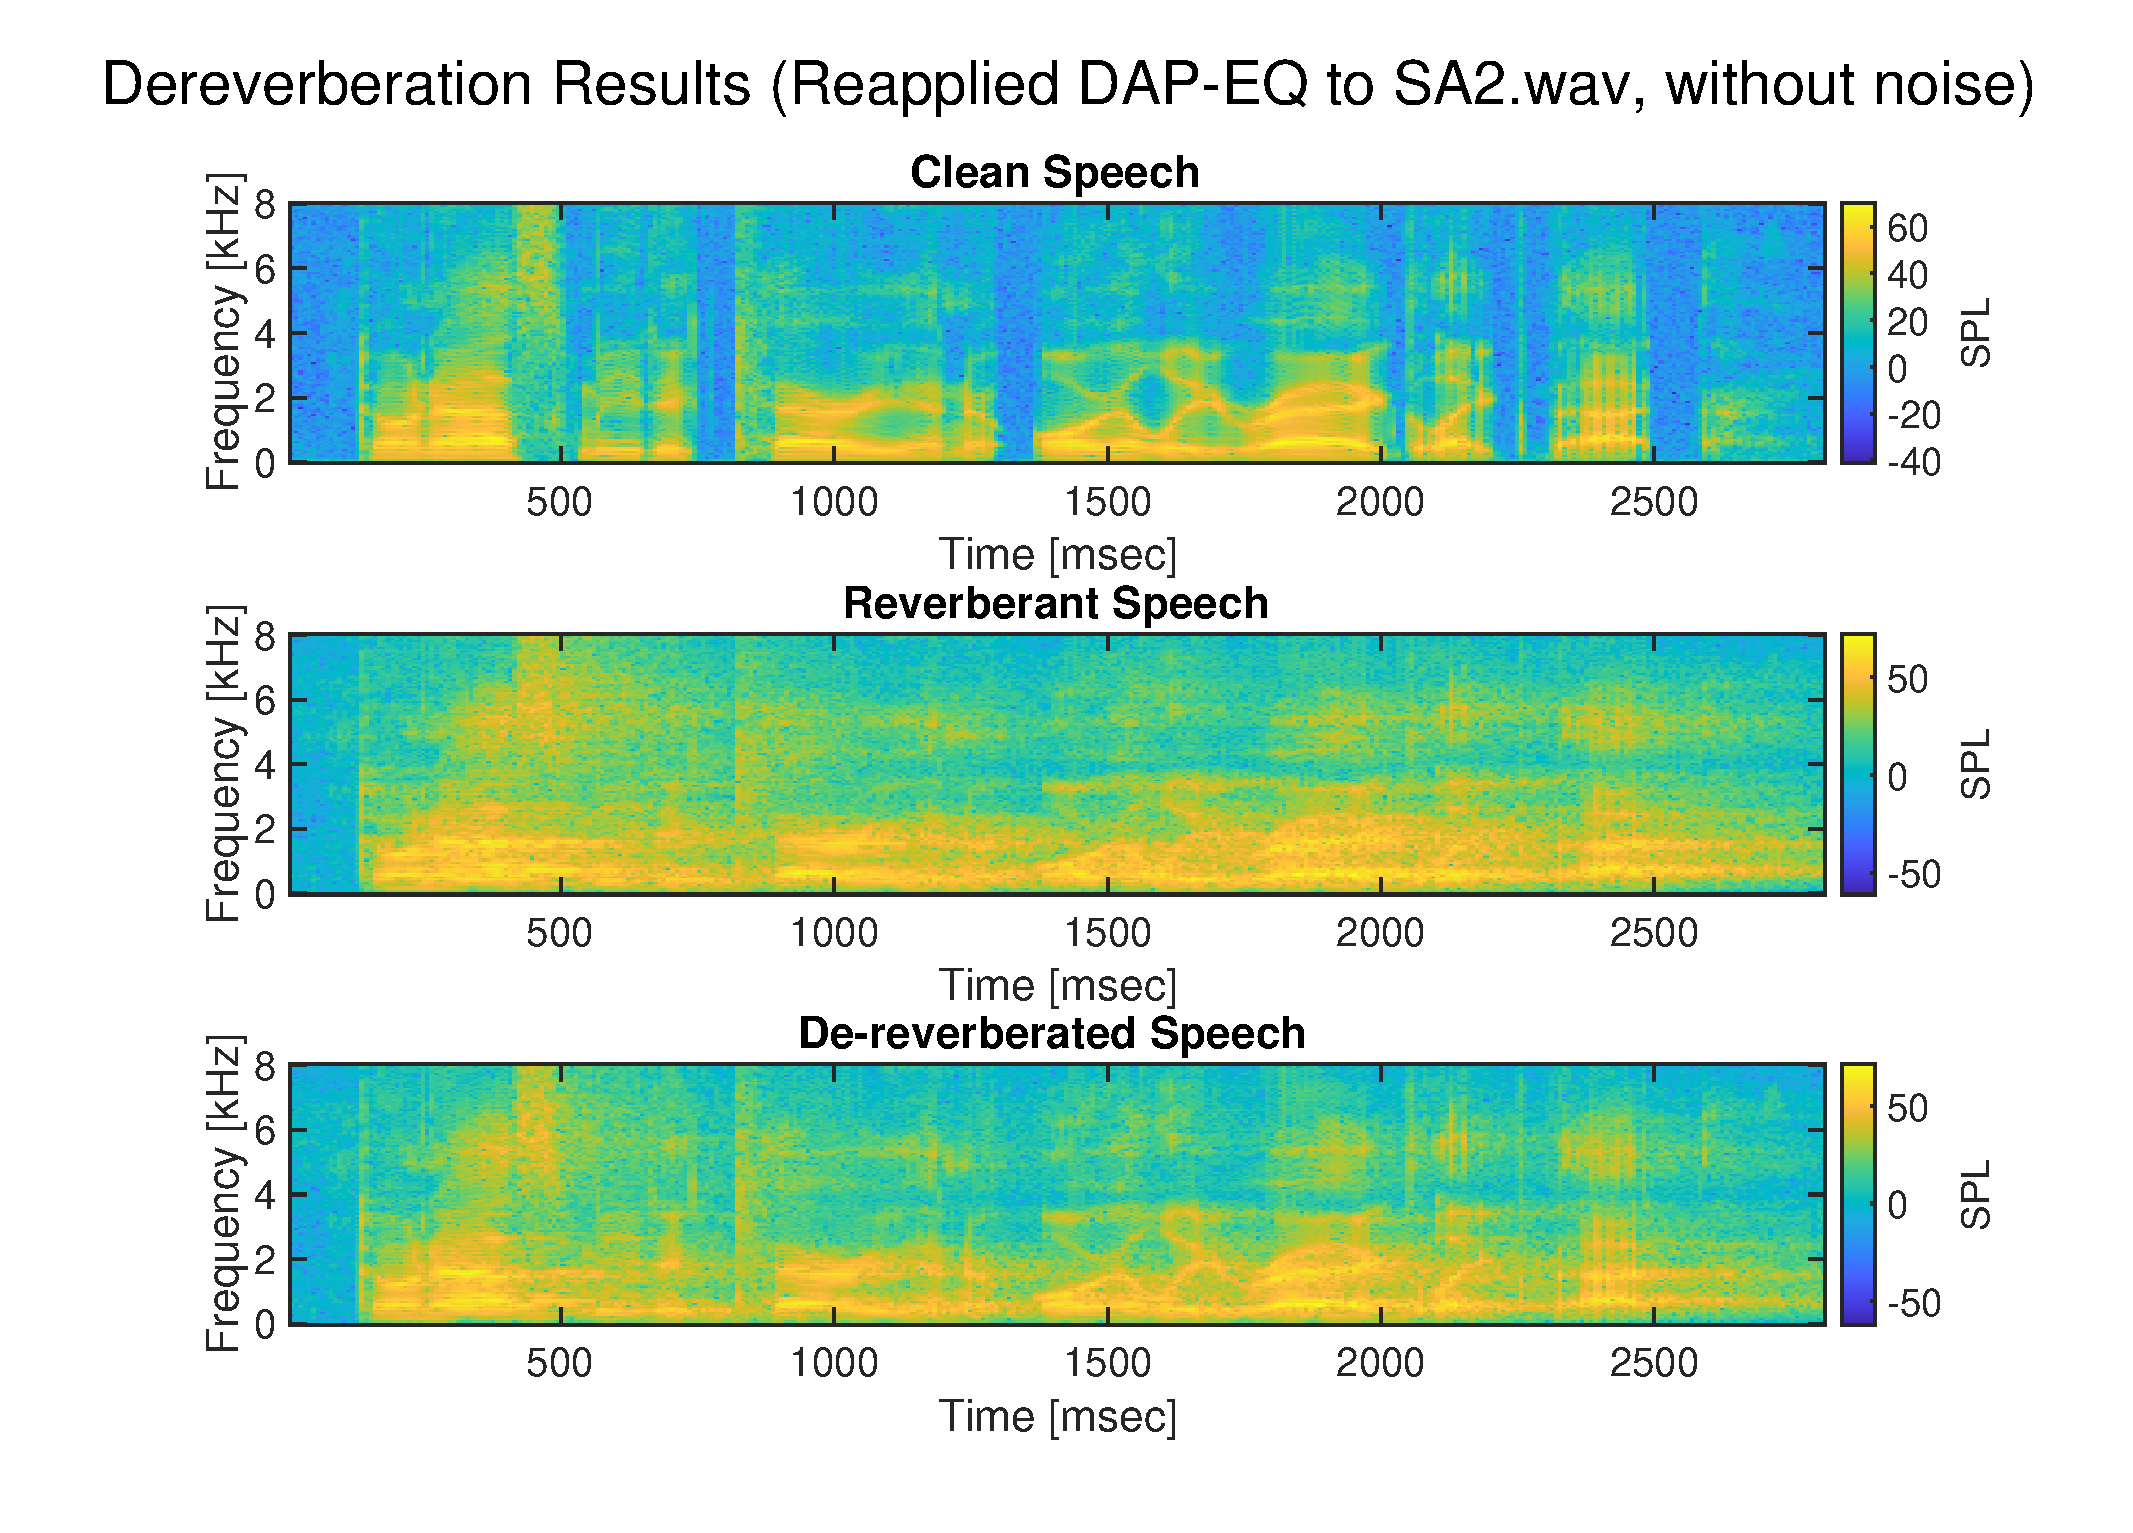
\includegraphics[width=\textwidth]{FullExample_Blind_Spectrogram}
	\end{subfigure}
	\caption[Blind DAP equalizer performance (EDC and spectrogram)]{DAP Equalizer performance (EDC and Spectrogram) with the source-whitening filter computed using reverberant speech (i.e., blind)}
	\label{fig:fullExample_Blind}
\end{figure}

As observed before, the MINT equalizer and the supervised DAP equalizer both produced EDCs that show a nearly instanteous substantial decay of reverberation. Like before, the EDC corresponding to the supervised DAP equalizer was observed to plateau around 30-35 \unit{\decibel} and to remain roughly flat over the time spanned by the equalizer length due to increased estimation variance at longer autocorrelation lags.

The EDC corresponding to the blind DAP equalizer (Figure \ref{fig:fullExample_Blind}) showed much less attenuation of the early part of the RIR (approximately \qty{6}{\decibel} attenuation). The EDC then continues to decay at approximately the same rate as the original RIR, until it levels out at a similar attenuation as the supervised case (approximately 30 -- 35 \unit{\decibel}), and similarly was observed to fall off at the end of the time spanned by the equalizer length. Thus the blind version of the DAP algorithm provides a similar result to the supervised version, but its performance is degraded by having to blindly estimate the source-whitening filter. The performance degradation was presumed to be due to common or near-common AR parameters (i.e., the effective poles) between the acoustic channels since RTFs tend to have some similarity in their frequency response, and due to the finite number of spatial sampling points (i.e., microphones) being used to average out the non-common AR parameters in the estimation of the source-whitening filter (i.e., Equation \ref{eq:dap_avg_autocorr}).

Looking at the spectrogram results, a clear benefit of all three equalizers was noted. For example, note that the diphthong around \qty{1500}{\milli\sec}, is almost completely obsecured by the smearing of reverberant energy (row 2), whereas it is more clearly defined in the spectrogram of the dereverberated speech signals (row 3) in all three cases. While this improvement is less pronounced in the blind DAP case than the MINT or supervised DAP cases, there is still a clear benefit of the algorithm.

\section{Number of Microphones}

To evaluate the impact of the number of microphones/channels, $M$, on performance, the $M$-channel RIR had to be generated synthetically since none of the RIR databases available had more than 6 channels. For this evaluation \qty{21.8}{\sec} of speech was used, exponentially decaying Gaussian RIRs were generated with $\mathrm{T60} = 100 \unit{\milli\second}$ and prediction orders of $p_2 = \mathrm{N60} / \left(M-1\right)$ and $p_1 = 1.25 \cdot p_2 \cdot \left(M-1\right)$ were used. The source whitening stage was trained on reverberant speech (i.e., fully blind). The results are shown in Figure \ref{fig:params_M_compare}.

\begin{figure}[H]
	\centering
	
	% ROW A
	\makebox[\textwidth][l]{%
		\begin{minipage}{0.08\textwidth}
			\centering
			\raggedleft{\footnotesize \textbf{(a)} \newline $M=2$} \\
		\end{minipage}%
		\begin{minipage}{0.91\textwidth}
			\begin{subfigure}[t]{0.32\textwidth}
				\centering
				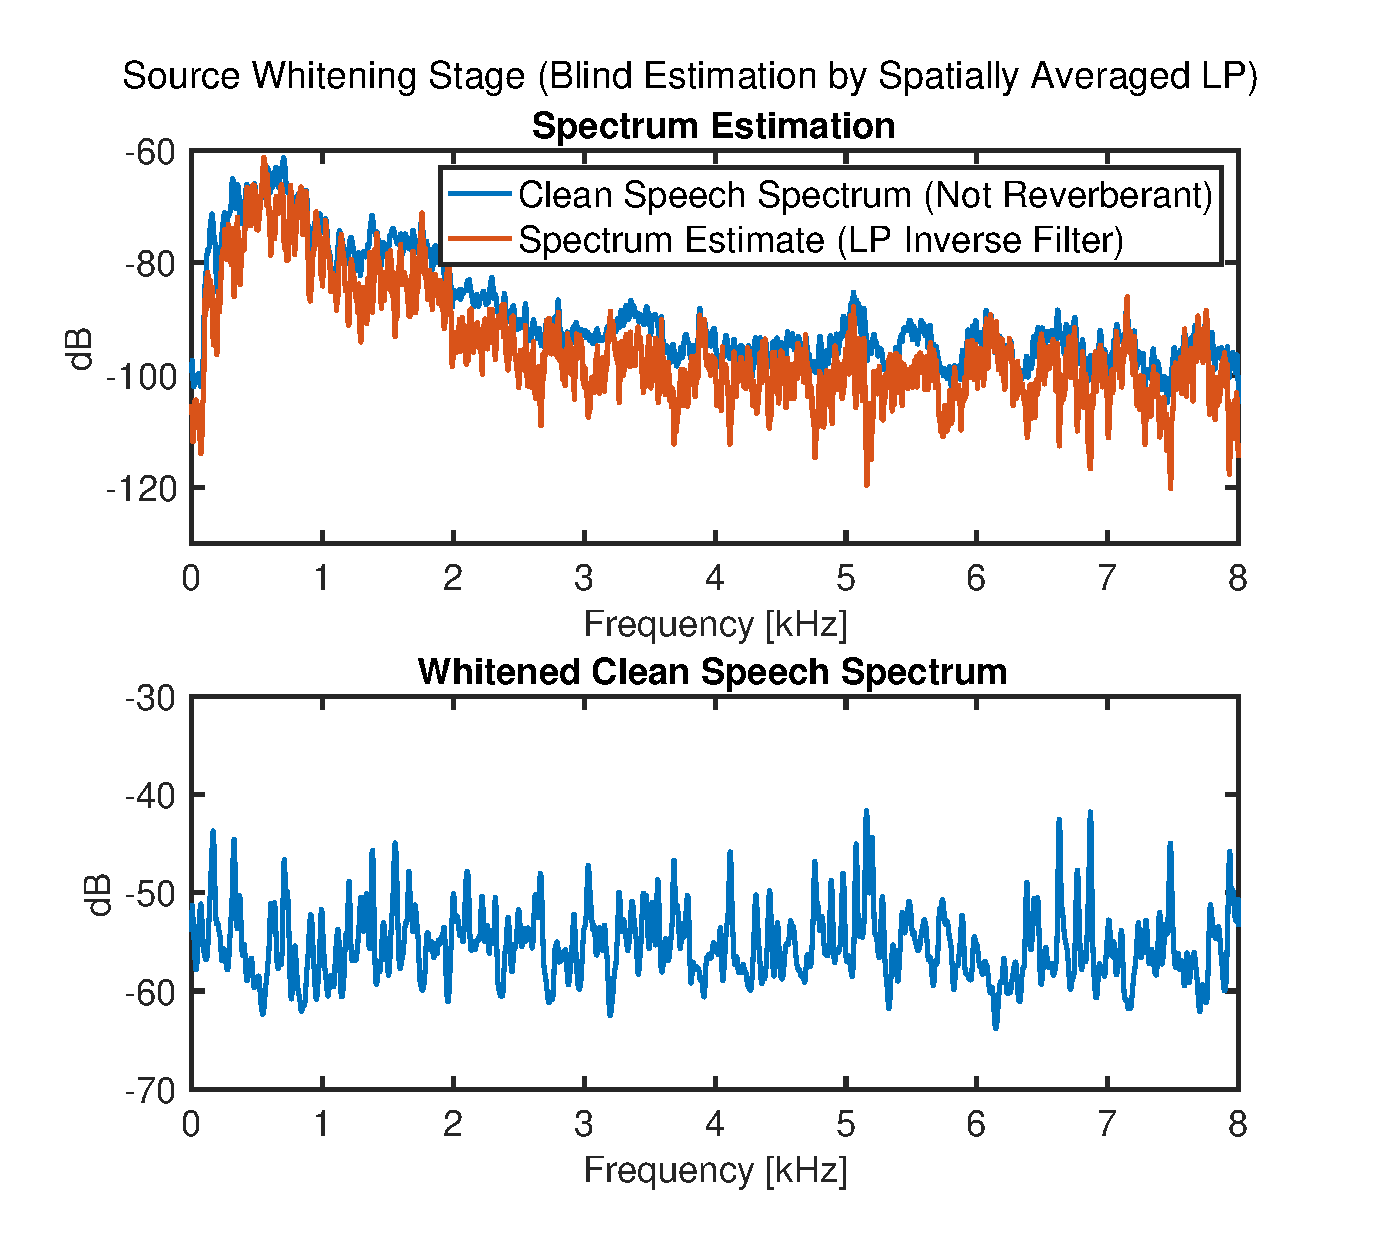
\includegraphics[width=\linewidth]{S1_M_2}
			\end{subfigure}
			\hfill
			\begin{subfigure}[t]{0.32\textwidth}
				\centering
				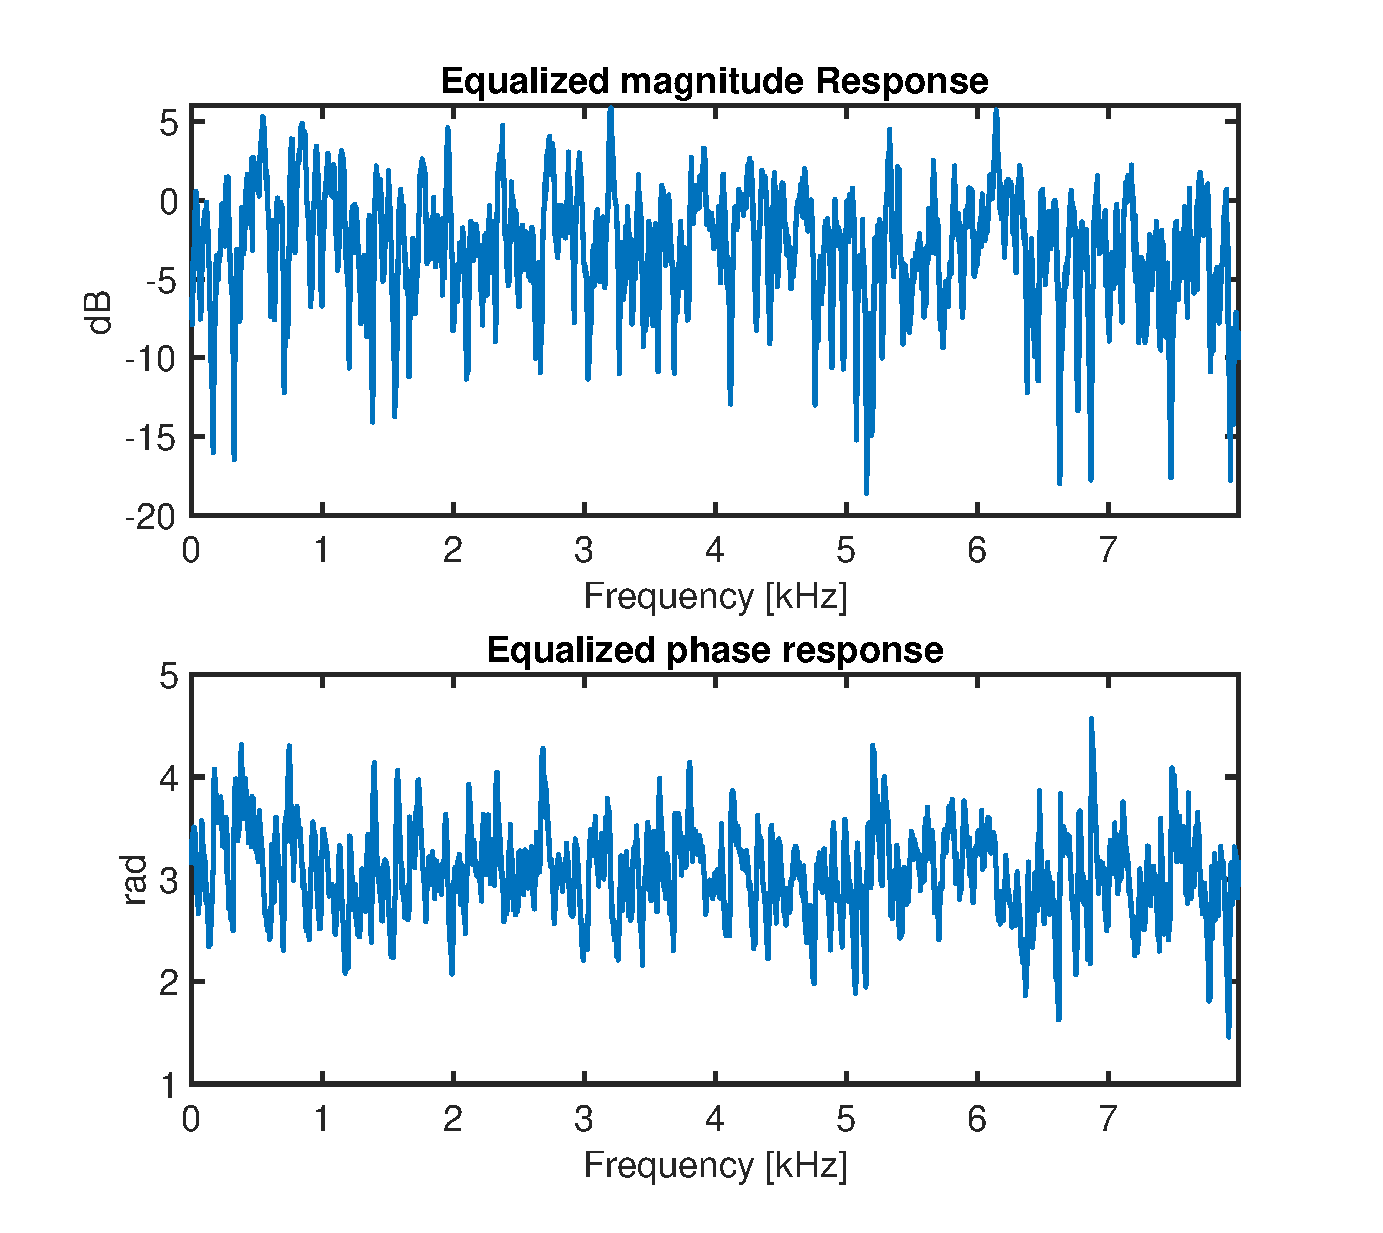
\includegraphics[width=\linewidth]{Equalized_RTF_M_2}
			\end{subfigure}
			\hfill
			\begin{subfigure}[t]{0.32\textwidth}
				\centering
				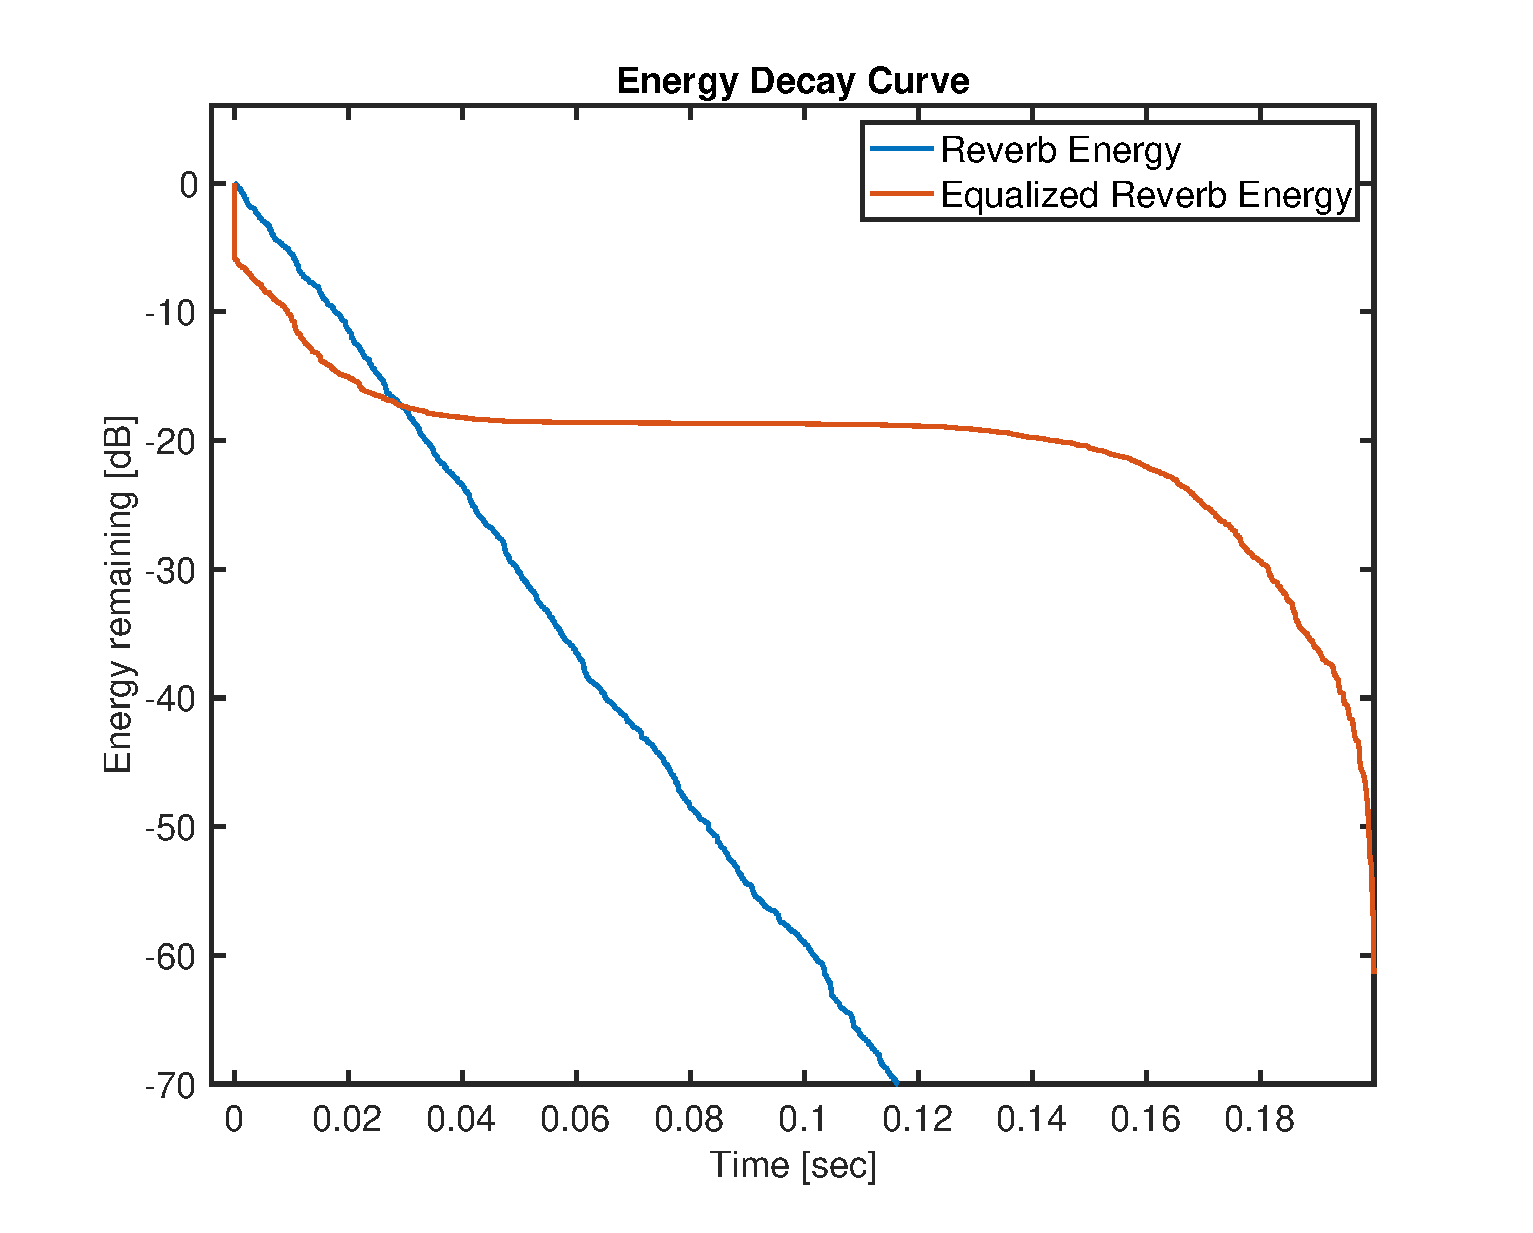
\includegraphics[width=\linewidth]{EDC_M_2}
			\end{subfigure}
		\end{minipage}
	}
	% Dummy subfigure for referencing row A
	\refstepcounter{subfigure}
	\label{subfig:params_M_compare:A}
	
	\vspace{1em}
	
	% ROW B
	\makebox[\textwidth][l]{%
		\begin{minipage}{0.08\textwidth}
			\centering
			\raggedleft{\footnotesize \textbf{(a)} \newline $M=4$} \\
		\end{minipage}%
		\begin{minipage}{0.91\textwidth}
			\begin{subfigure}[t]{0.32\textwidth}
				\centering
				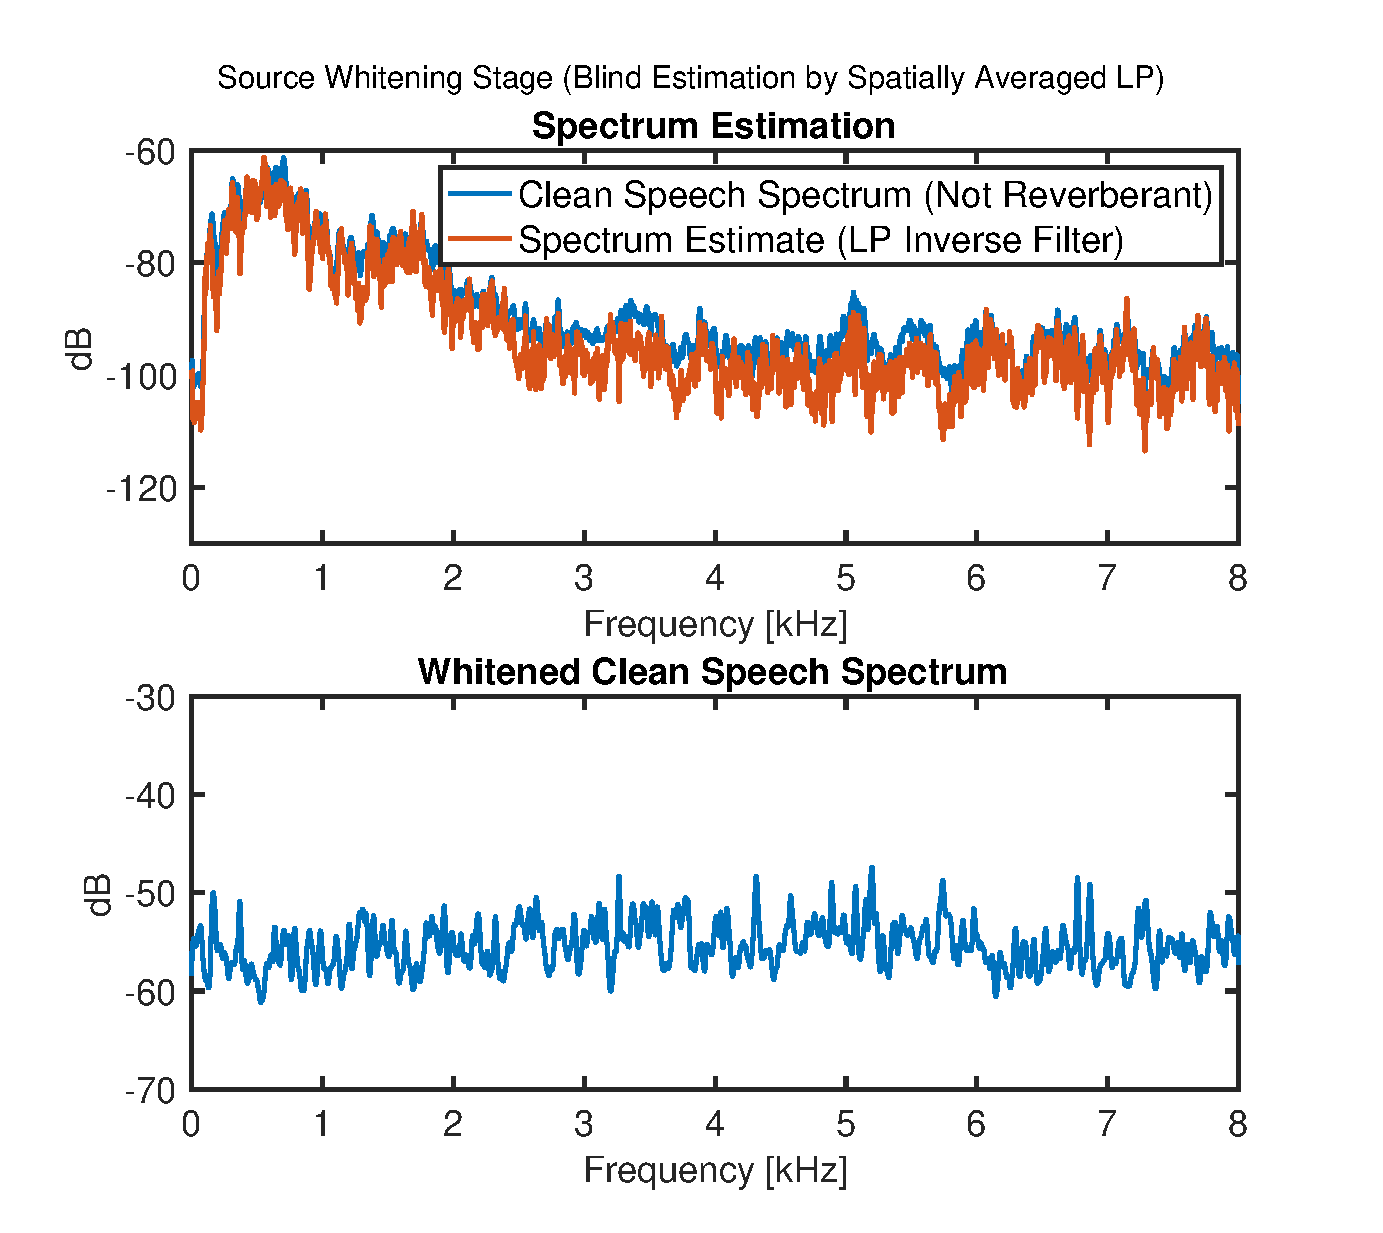
\includegraphics[width=\linewidth]{S1_M_4}
			\end{subfigure}
			\hfill
			\begin{subfigure}[t]{0.32\textwidth}
				\centering
				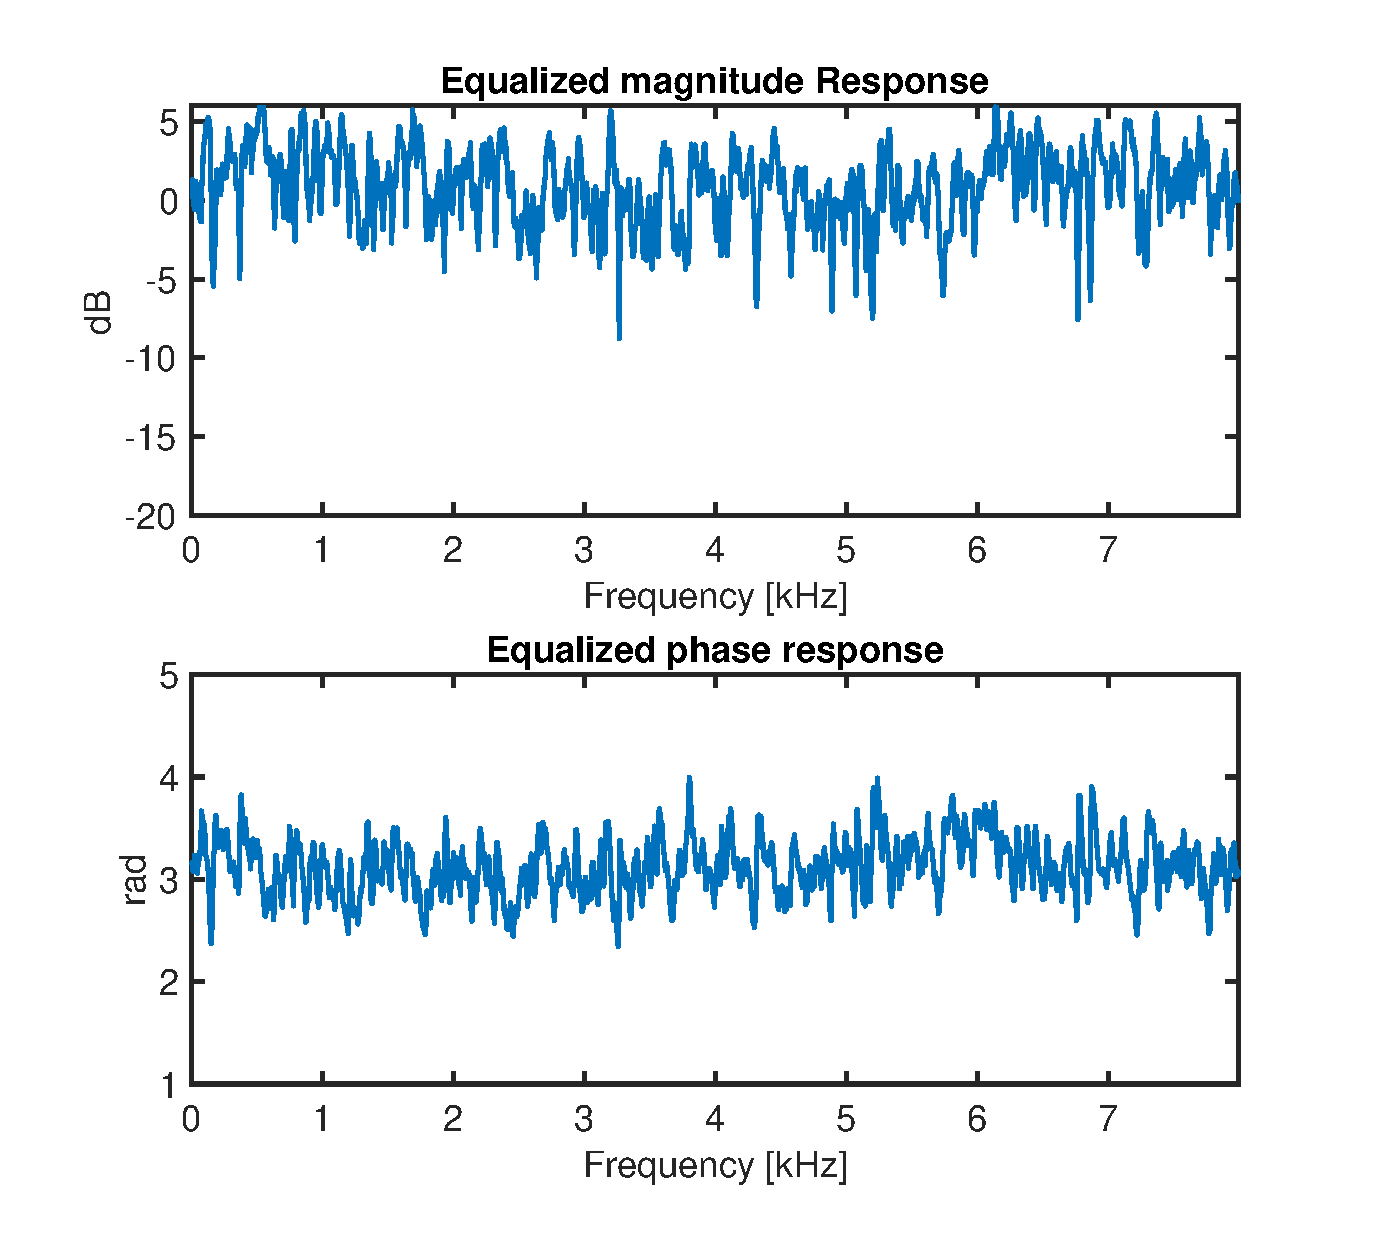
\includegraphics[width=\linewidth]{Equalized_RTF_M_4}
			\end{subfigure}
			\hfill
			\begin{subfigure}[t]{0.32\textwidth}
				\centering
				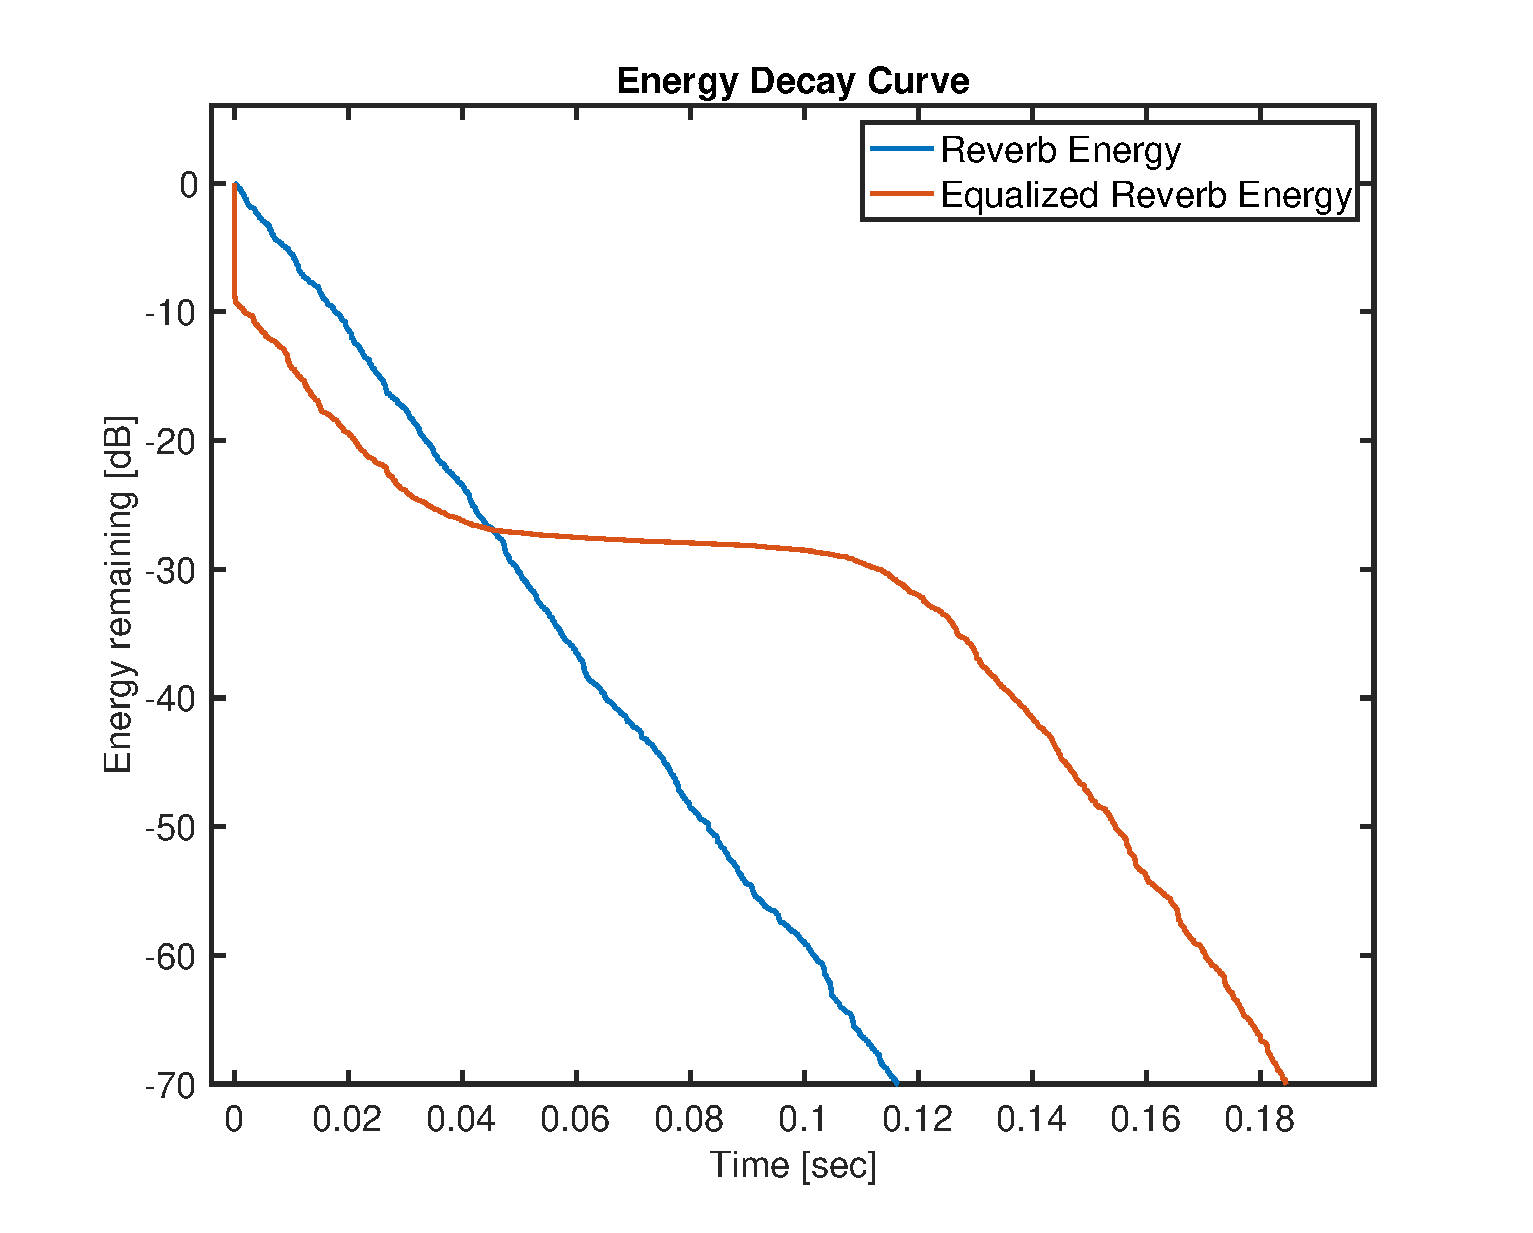
\includegraphics[width=\linewidth]{EDC_M_4}
			\end{subfigure}
		\end{minipage}
	}
	% Dummy subfigure for referencing row B
	\refstepcounter{subfigure}
	\label{subfig:params_M_compare:B}
	
	\vspace{1em}
	
	% ROW C
	\makebox[\textwidth][l]{%
		\begin{minipage}{0.08\textwidth}
			\centering
			\raggedleft{\footnotesize \textbf{(a)} \newline $M=8$} \\
		\end{minipage}%
		\begin{minipage}{0.91\textwidth}
			\begin{subfigure}[t]{0.32\textwidth}
				\centering
				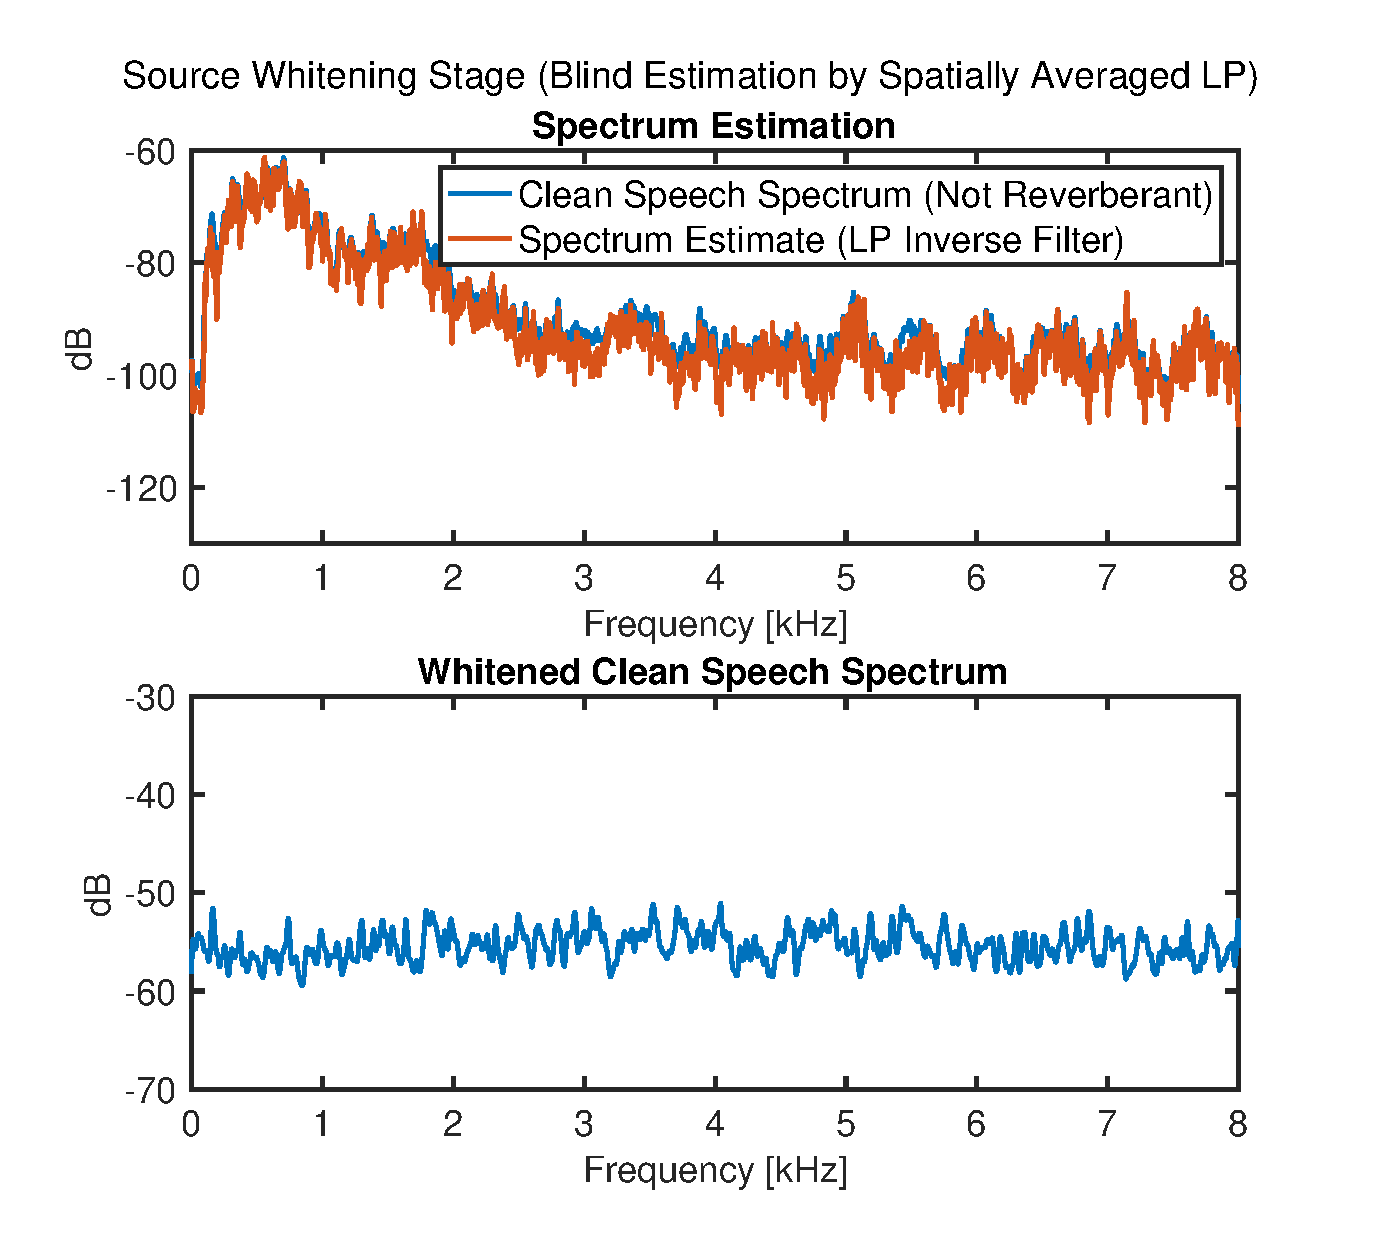
\includegraphics[width=\linewidth]{S1_M_8}
			\end{subfigure}
			\hfill
			\begin{subfigure}[t]{0.32\textwidth}
				\centering
				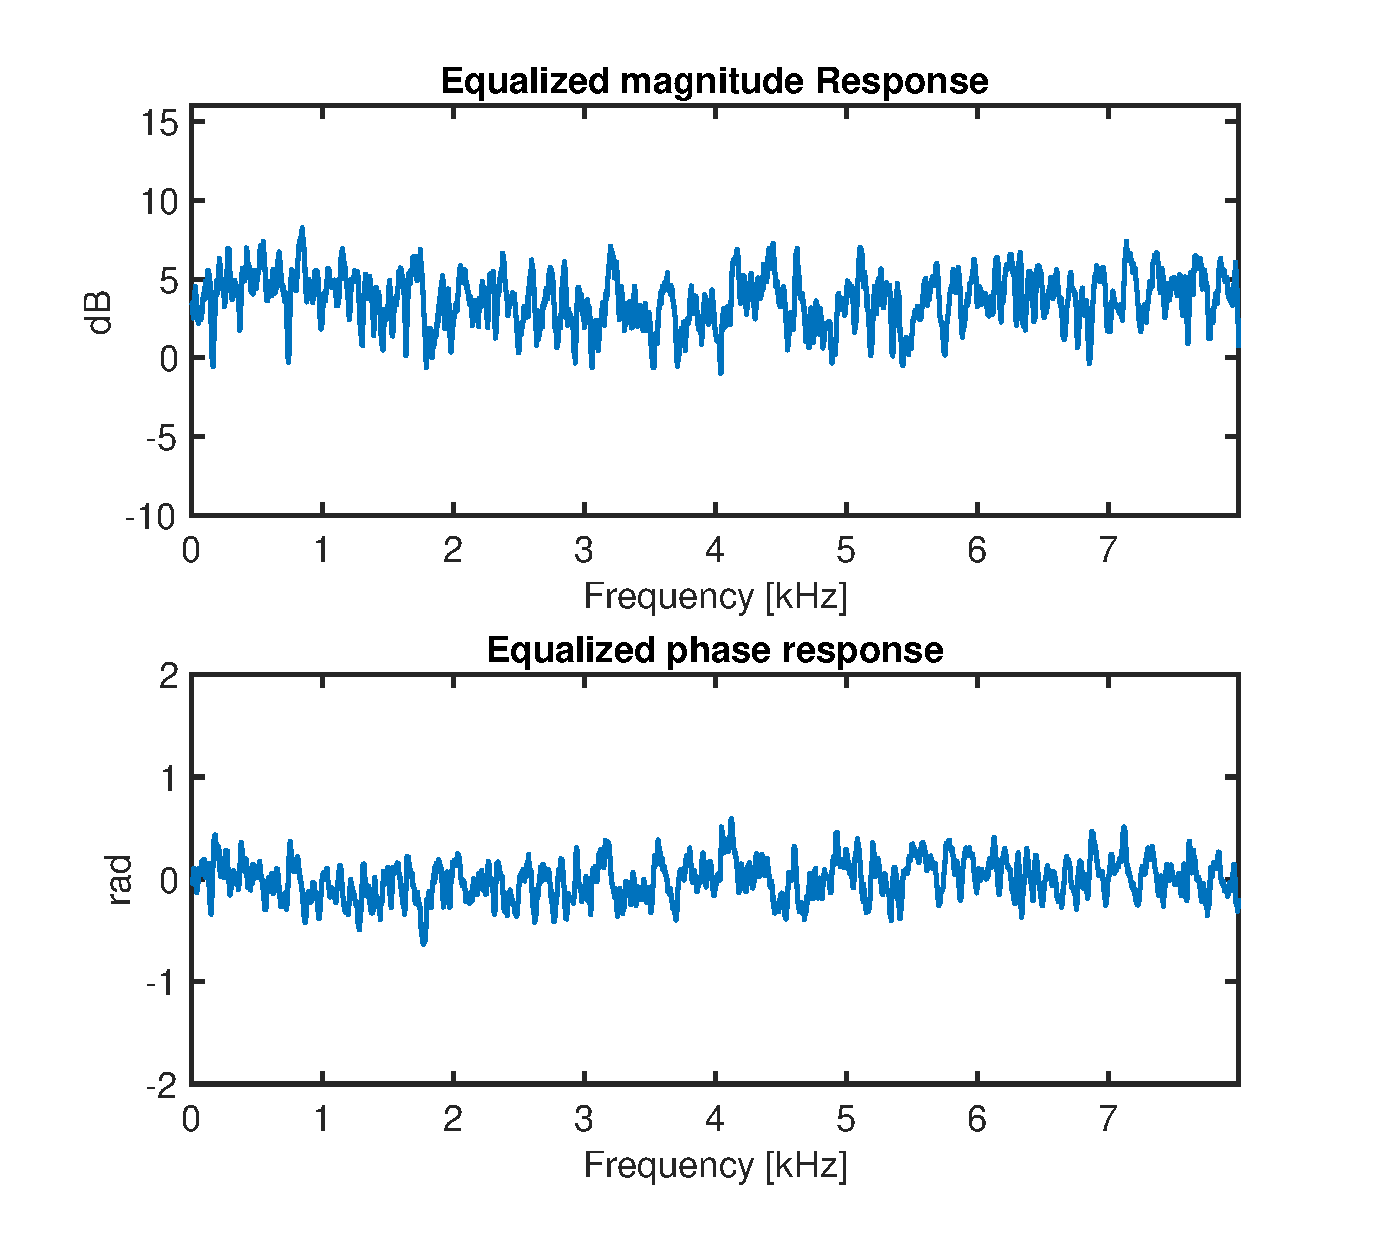
\includegraphics[width=\linewidth]{Equalized_RTF_M_8}
			\end{subfigure}
			\hfill
			\begin{subfigure}[t]{0.32\textwidth}
				\centering
				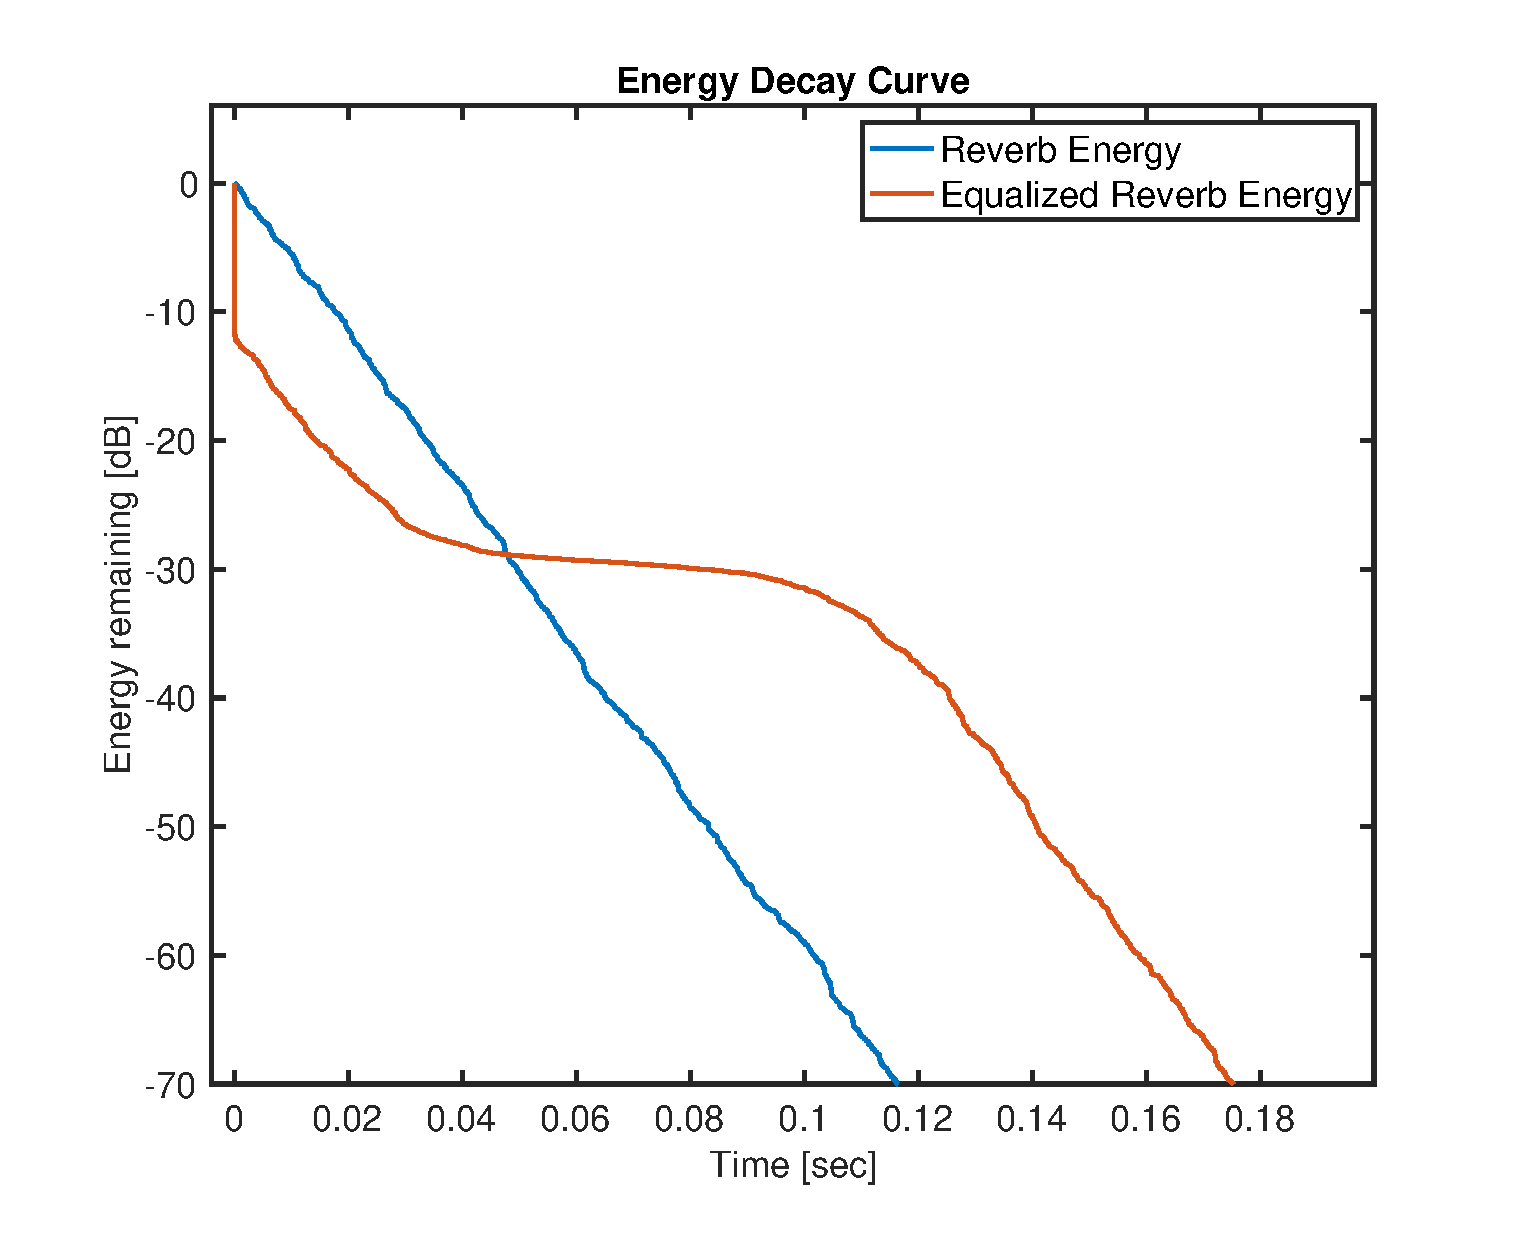
\includegraphics[width=\linewidth]{EDC_M_8}
			\end{subfigure}
		\end{minipage}
	}
	% Dummy subfigure for referencing row C
	\refstepcounter{subfigure}
	\label{subfig:params_M_compare:C}
	
	\vspace{1em}
	
	% ROW D
	\makebox[\textwidth][l]{%
		\begin{minipage}{0.08\textwidth}
			\centering
			\raggedleft{\footnotesize \textbf{(a)} \newline $M=16$} \\
		\end{minipage}%
		\begin{minipage}{0.91\textwidth}
			\begin{subfigure}[t]{0.32\textwidth}
				\centering
				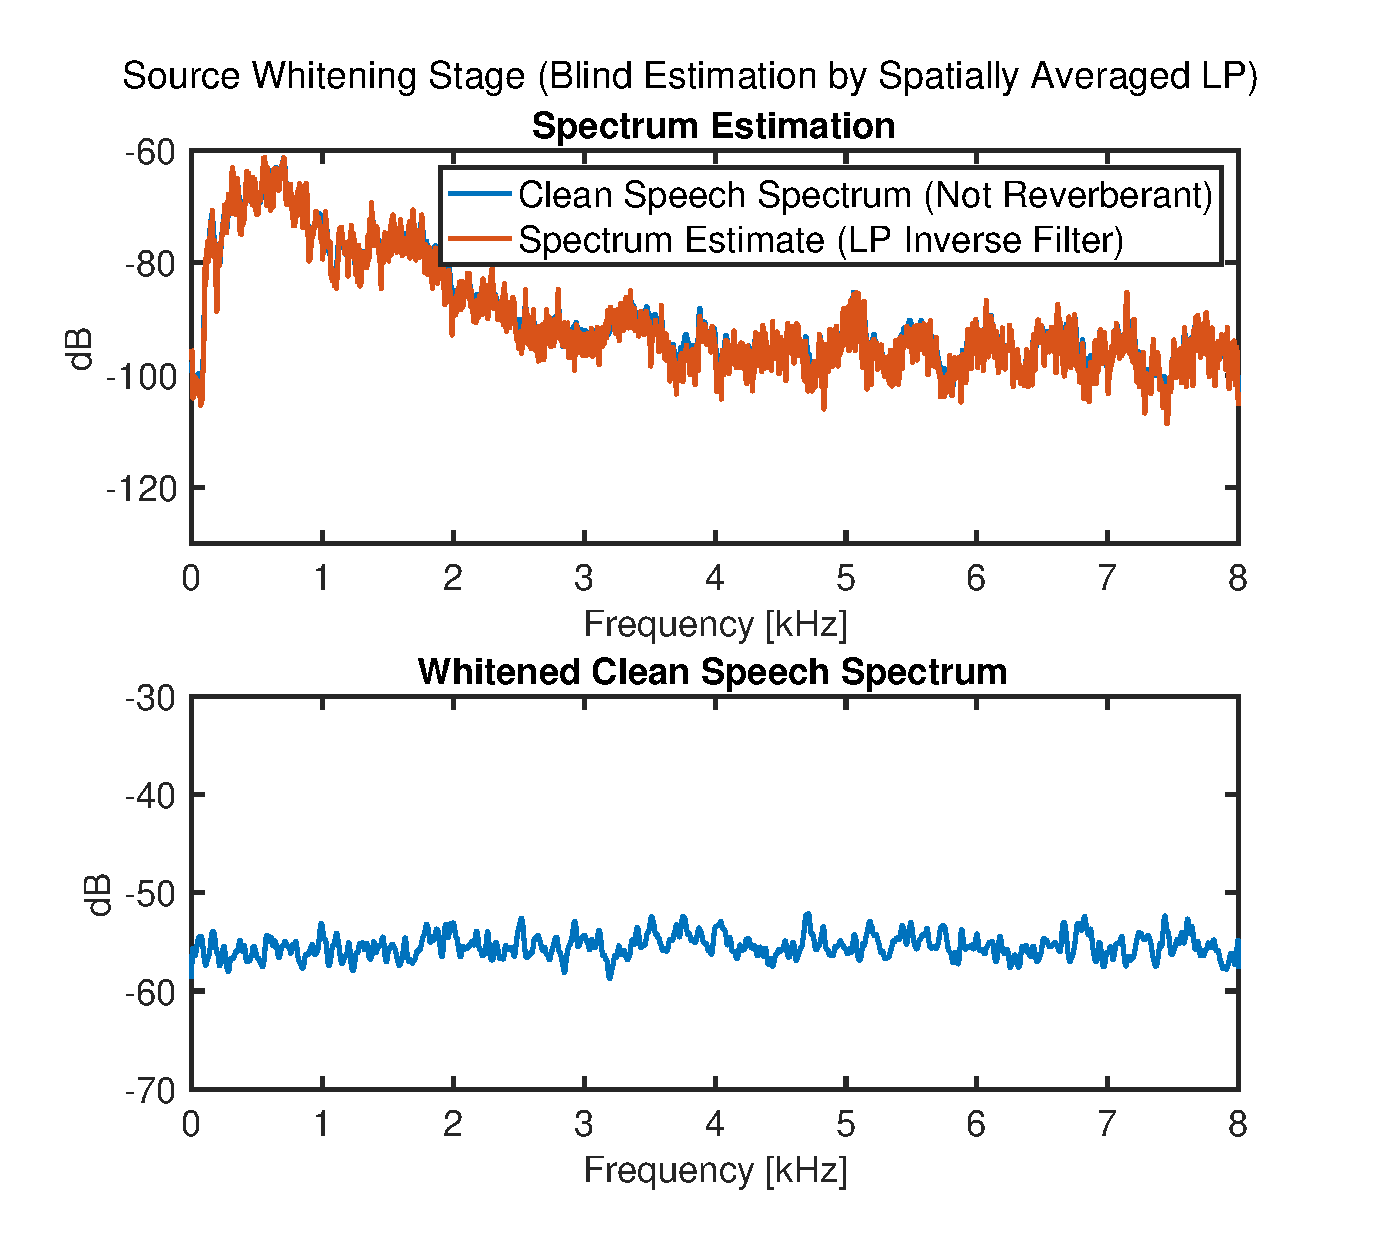
\includegraphics[width=\linewidth]{S1_M_16}
			\end{subfigure}
			\hfill
			\begin{subfigure}[t]{0.32\textwidth}
				\centering
				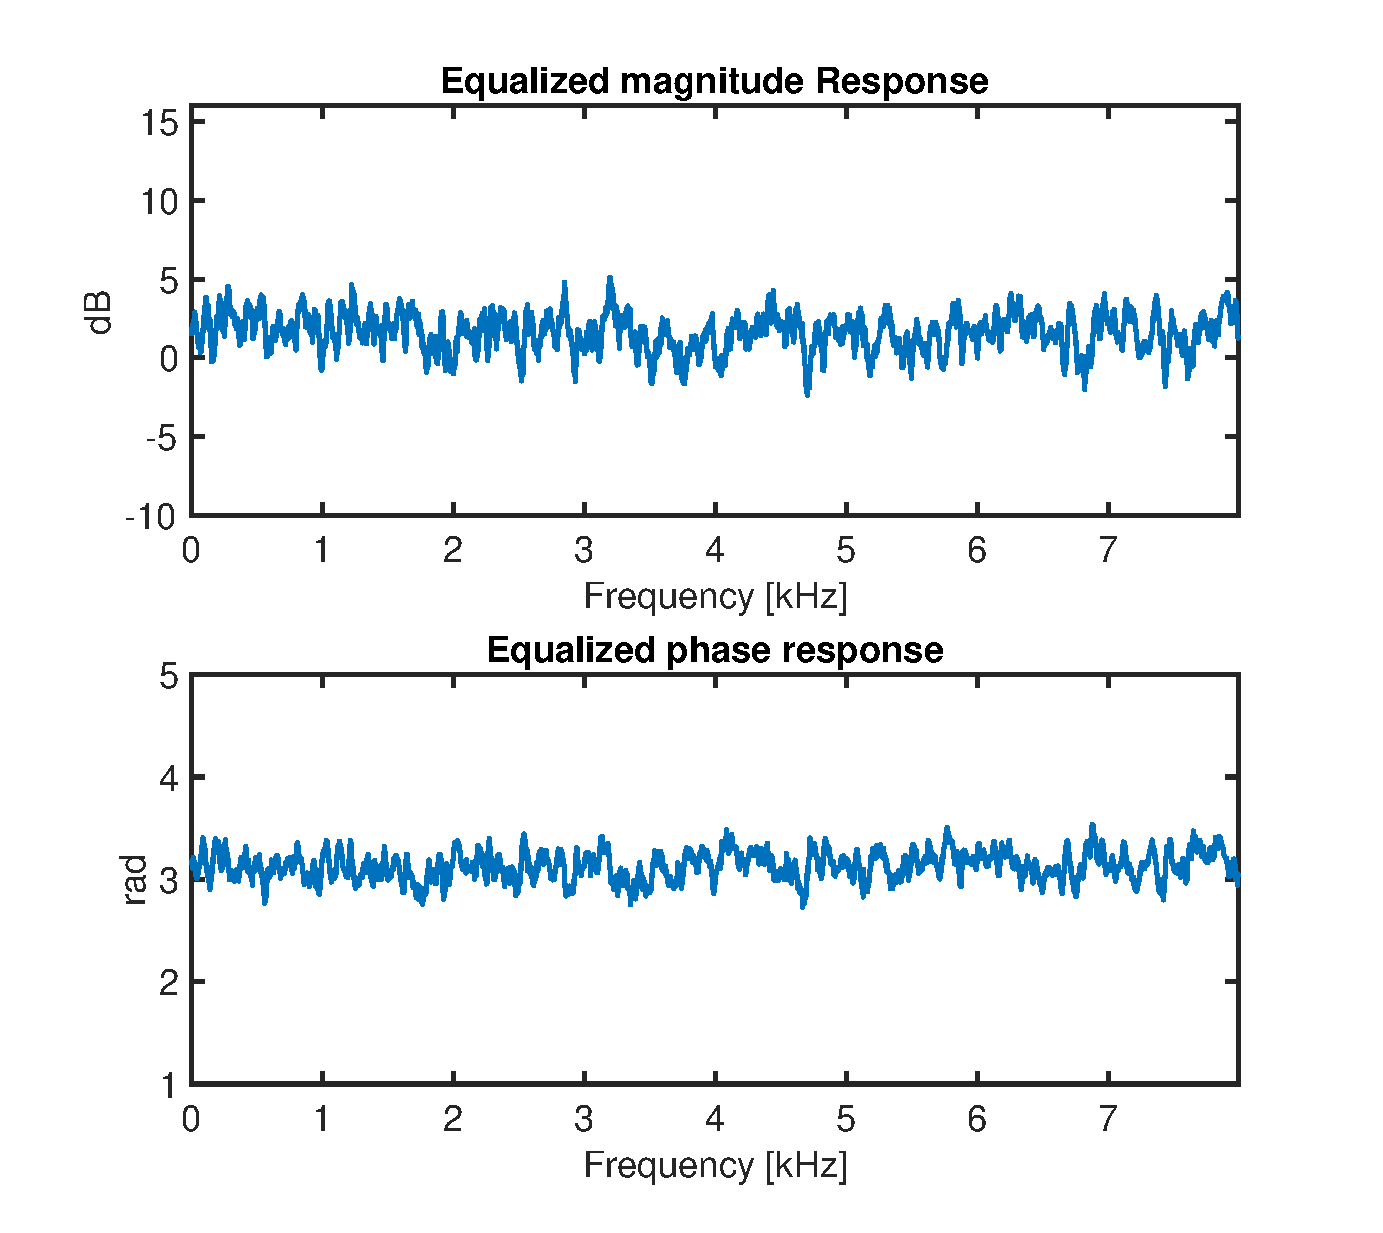
\includegraphics[width=\linewidth]{Equalized_RTF_M_16}
			\end{subfigure}
			\hfill
			\begin{subfigure}[t]{0.32\textwidth}
				\centering
				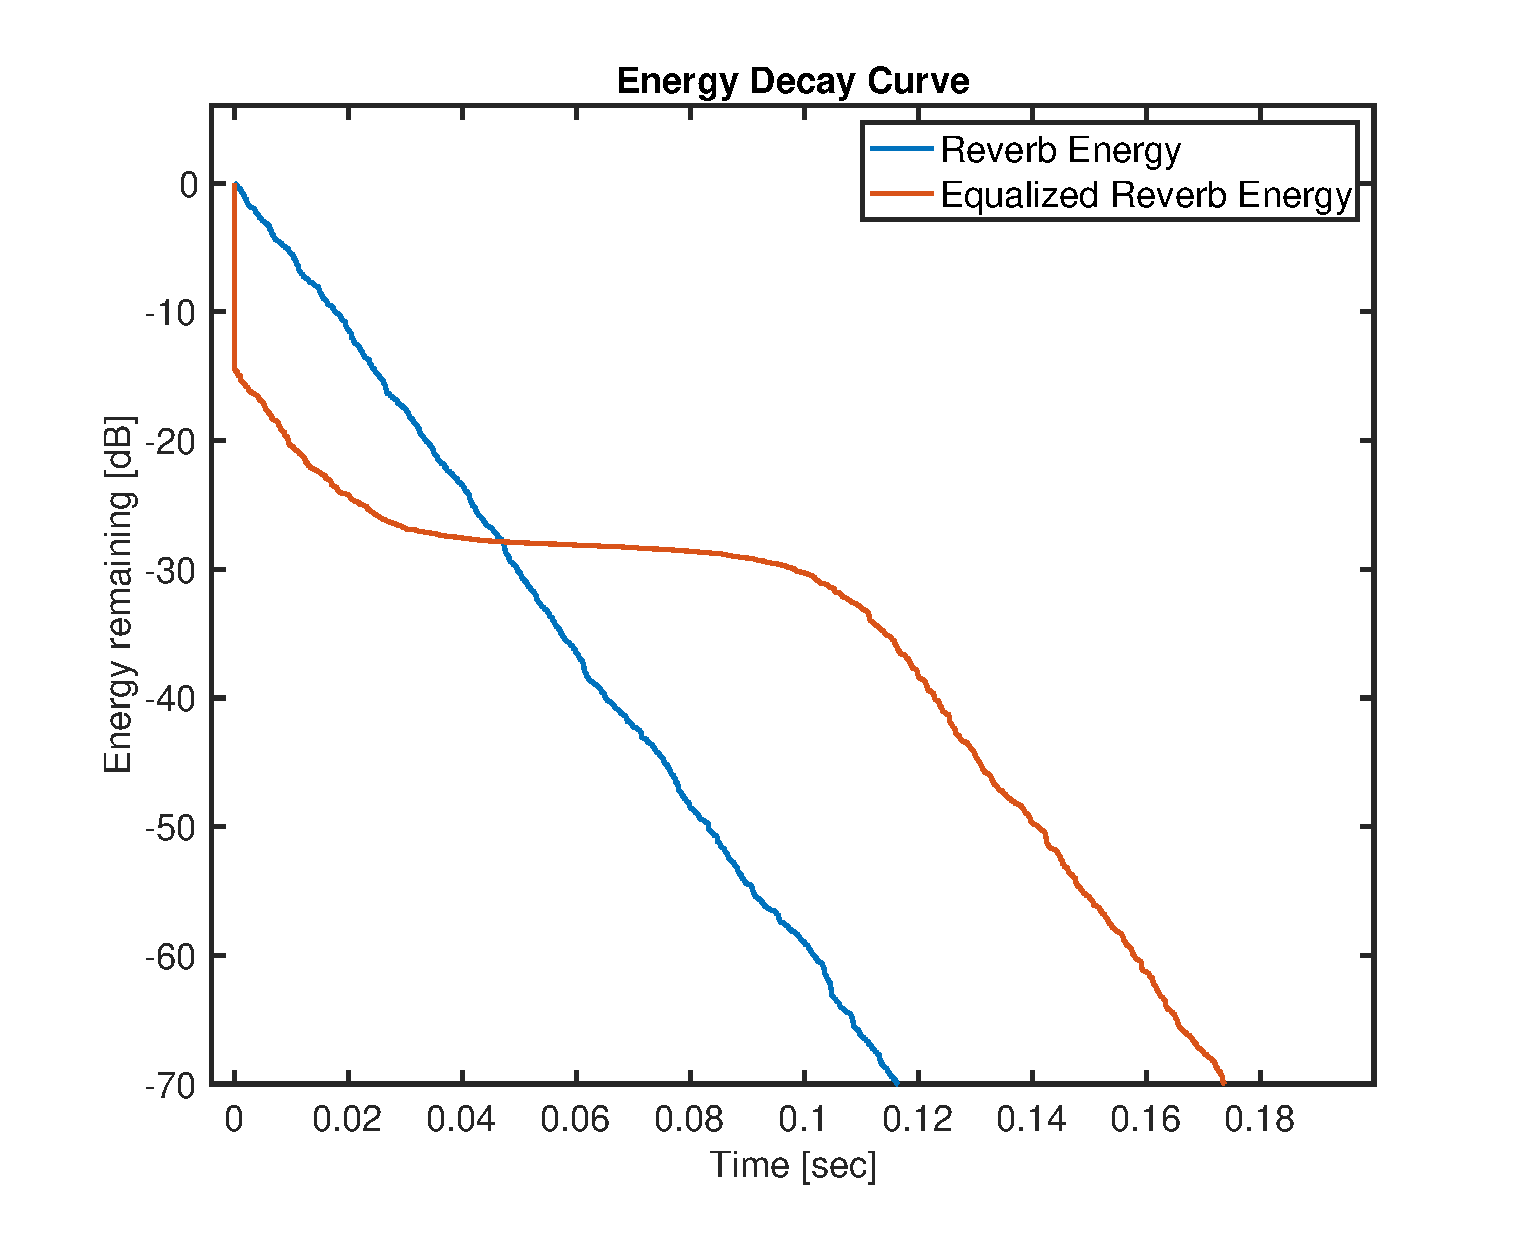
\includegraphics[width=\linewidth]{EDC_M_16}
			\end{subfigure}
		\end{minipage}
	}
	% Dummy subfigure for referencing row D
	\refstepcounter{subfigure}
	\label{subfig:params_M_compare:D}
	
	\caption[Impact of number of microphones on DAP dereverberation performance]{Impact of number of microphones $M$ on DAP dereverberation performance. Source whitening prediction order was $\mathrm{p_1} = 1.25 \cdot \mathrm{p_2} \cdot (M-1)$ and MC-LP order was $\mathrm{p_2} = \mathrm{N60} / (M-1)$. Source Whitening stage was performed on reverberant speech (i.e., blind estimation). RIRs were synthetically generated exponentially decaying Gaussians.}
	\label{fig:params_M_compare}
	
\end{figure}

A significant increase in performance was observed in all three columns as the number of microphones was increased. This makes sense because the blind estimation of the source spectrum (Equation \ref{eq:dap_avg_autocorr}), which averages autocorrelation accross the spatial sampling points, requires many microphones to average out the effects of the channels. Additionally, increasing the number of microphones decreases the likelihood that channels will have common or numerically similar poles/zeros. This is particularly evident in the source-whitening results (column 1): the source spectrum was only whitened to approximately $\pm \qty{10}{\decibel}$ for $M=2$, versus approximately $\pm \qty{5}{\decibel}$ for $M=16$. A similar impact was observed on how flat the equalized magnitude/phase response (column 2). In terms of EDC results (column 3), using more microphones was found to only improve cancellation of the stronger early part of the RIR, having minimal impact on equalization of the late tail. This makes sense since increasing the number of microphones only improves the spatial averaging of the source spectrum, and does not have any impact on the estimation variance that arises at longer autocorrelation lags / weaker reverberation-to-noise ratios. In other words, as the number of microphones increases, the performance of the blind DAP algorithm converges towards the performance of the supervised DAP algorithm.

\section{Source Properties}

Two properties of the source speech stimulus were analyzed: source data length (i.e., length of the source sequence), and its spectral colouration. It was hypothesized that larger amounts of source data would decrease variance in the estimates of the autocorrelation functions used for both linear prediction stages, improving performance. It was also hypothesized that the amount of colour (i.e., the ``peakiness") of the source spectrum would have a negative impact on performance due to the increased demand on the source-whitening stage, and due to the known fact that the condition number of autocorrelation matrices is proportional to the signals spectral dynamic range which results in worse-conditioned normal equations for more ``peaky" spectra \citep{farhang2013adaptive}.

Since the power spectrum of a signal generally becomes smoother as sequence length increases, the evaluation method had to be designed carefully to isolate these two properties.  

In both evaluations, the four-channel RIR was the ``SAL" room from the MYRiAD database, exponentially windowed to $\mathrm{T60} = 100 \unit{\milli\second}$, and predictionorders were $p_2 = \mathrm{N60} / \left(M-1\right)$ and $p_1 = 2 \cdot p_2 \cdot \left(M-1\right)$. The fully blind DAP algorithm was used in this evaluation.


\subsection{Source Data Length} \label{section:params_source_length}

To test the source data length, the same \qty{3.6}{\sec} speech sample from the TMIT database was used in each test case, but was looped synthetically (1, 2, 3 and 4 times respectively) to the desired data length. In this way, the data length was increased without changing the spectrum. The results for each case are shown in Figure \ref{fig:params_source_length_compare}. The first column shows the performance of the source-whitening stage. The second column shows the equalized magnitude/phase response generated by taking the fourier transform of the EIR. The third column shows the resulting EDC.

%Test: Same spectrum different length
% -     Blind DAP
% - 	Speech is SA1.wav looped X times
% - 	RIR = SAL truncated to 100 msec = 1600 samples, M = 4 mics
% -     P1 = 2 * p2 * (M-1)
% - 	P2 = N60 / (M-1)
% - 	Reran exact same test for longer source sequences generated by looping SA1 – Exact same spectrum just more data (excludes spectrum dependency)


% Source Data Length Compare, Length = [(1x) 58061,  (2x) 116122, (3x) 174183, (4x) 232244 ], Blind

\begin{figure}[H]
	\centering
	
	% ROW A
	\makebox[\textwidth][l]{%
		\begin{minipage}{0.08\textwidth}
			\centering
			\raggedleft{\footnotesize \textbf{(a)} \newline \qty{3.6}{\sec} \newline source} \\
		\end{minipage}%
		\begin{minipage}{0.91\textwidth}
			\begin{subfigure}[t]{0.32\textwidth}
				\centering
				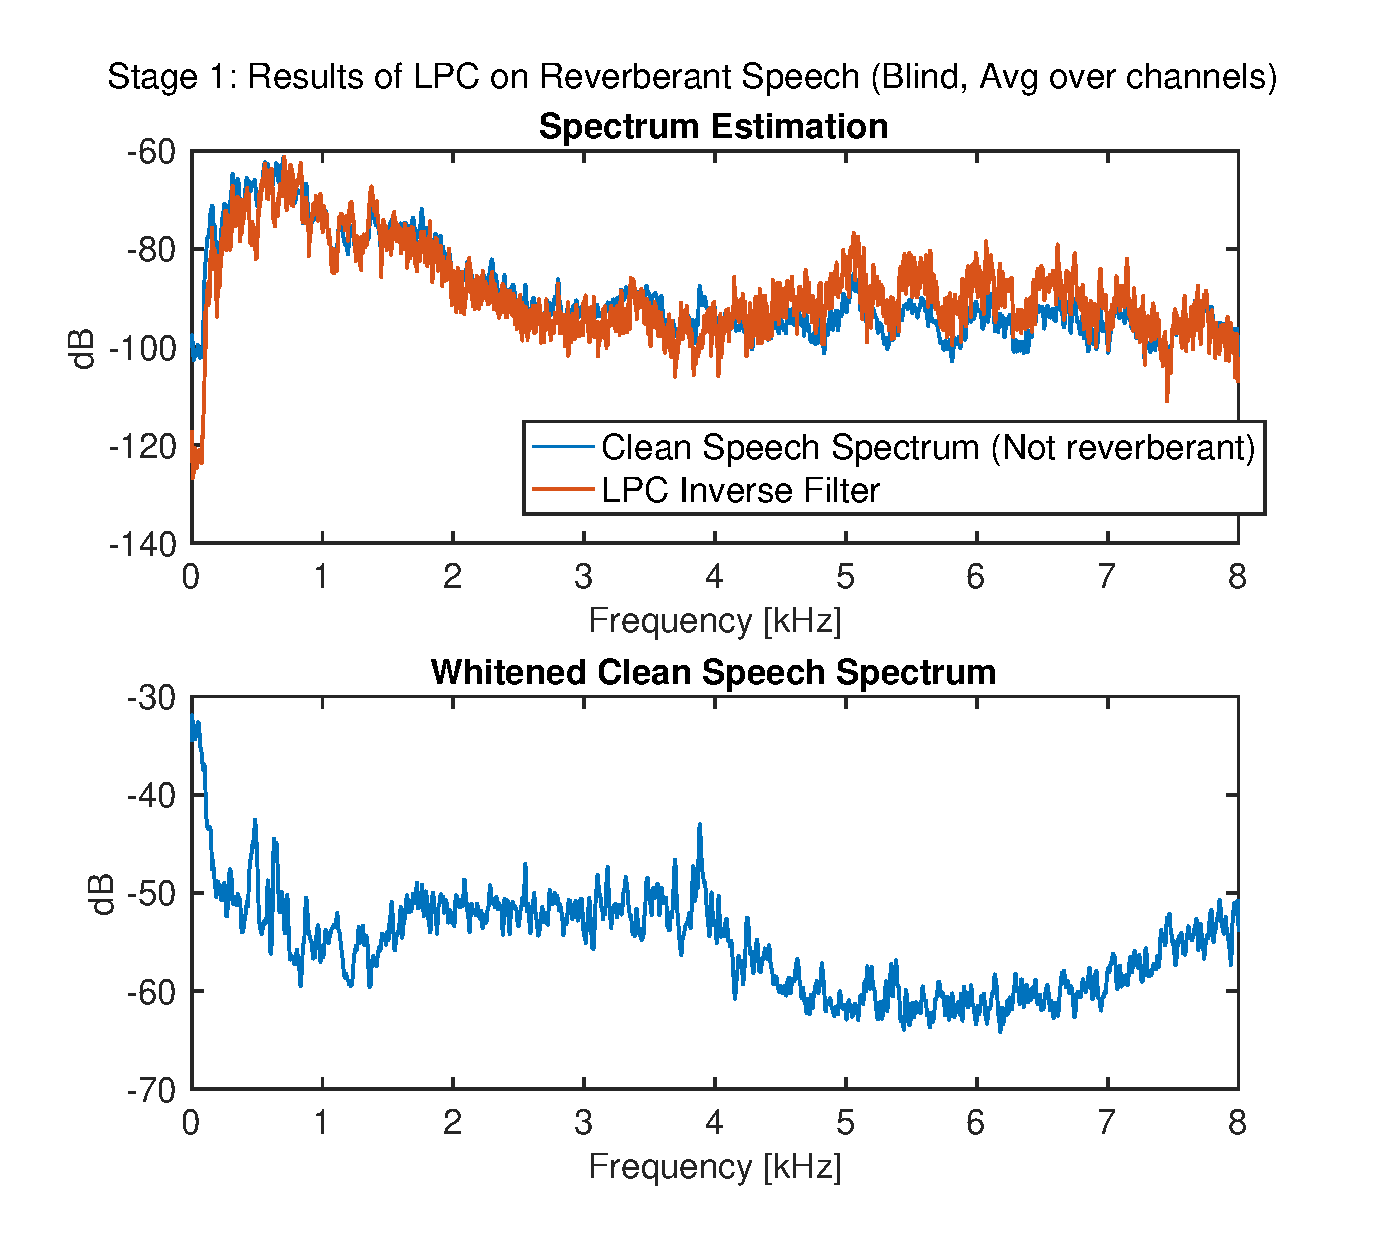
\includegraphics[width=\linewidth]{S1_SourceLength_1_Blind}
			\end{subfigure}
			\hfill
			\begin{subfigure}[t]{0.32\textwidth}
				\centering
				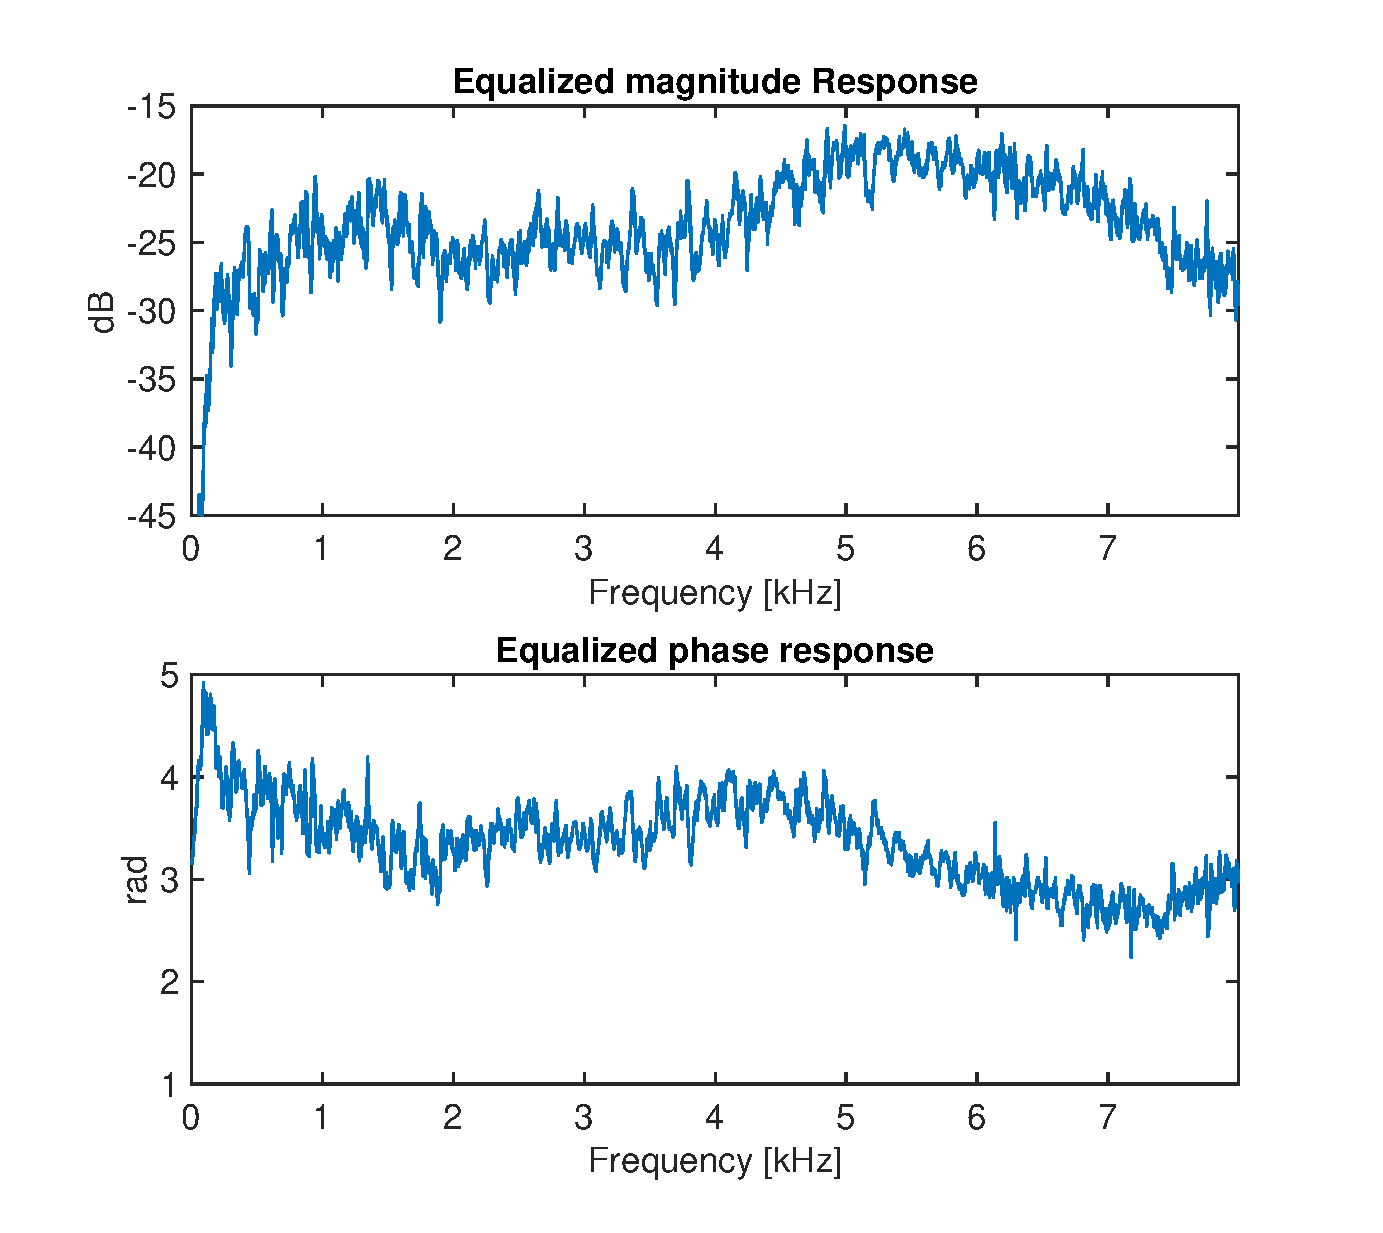
\includegraphics[width=\linewidth]{Equalized_RTF_SourceLength_1_Blind}
			\end{subfigure}
			\hfill
			\begin{subfigure}[t]{0.32\textwidth}
				\centering
				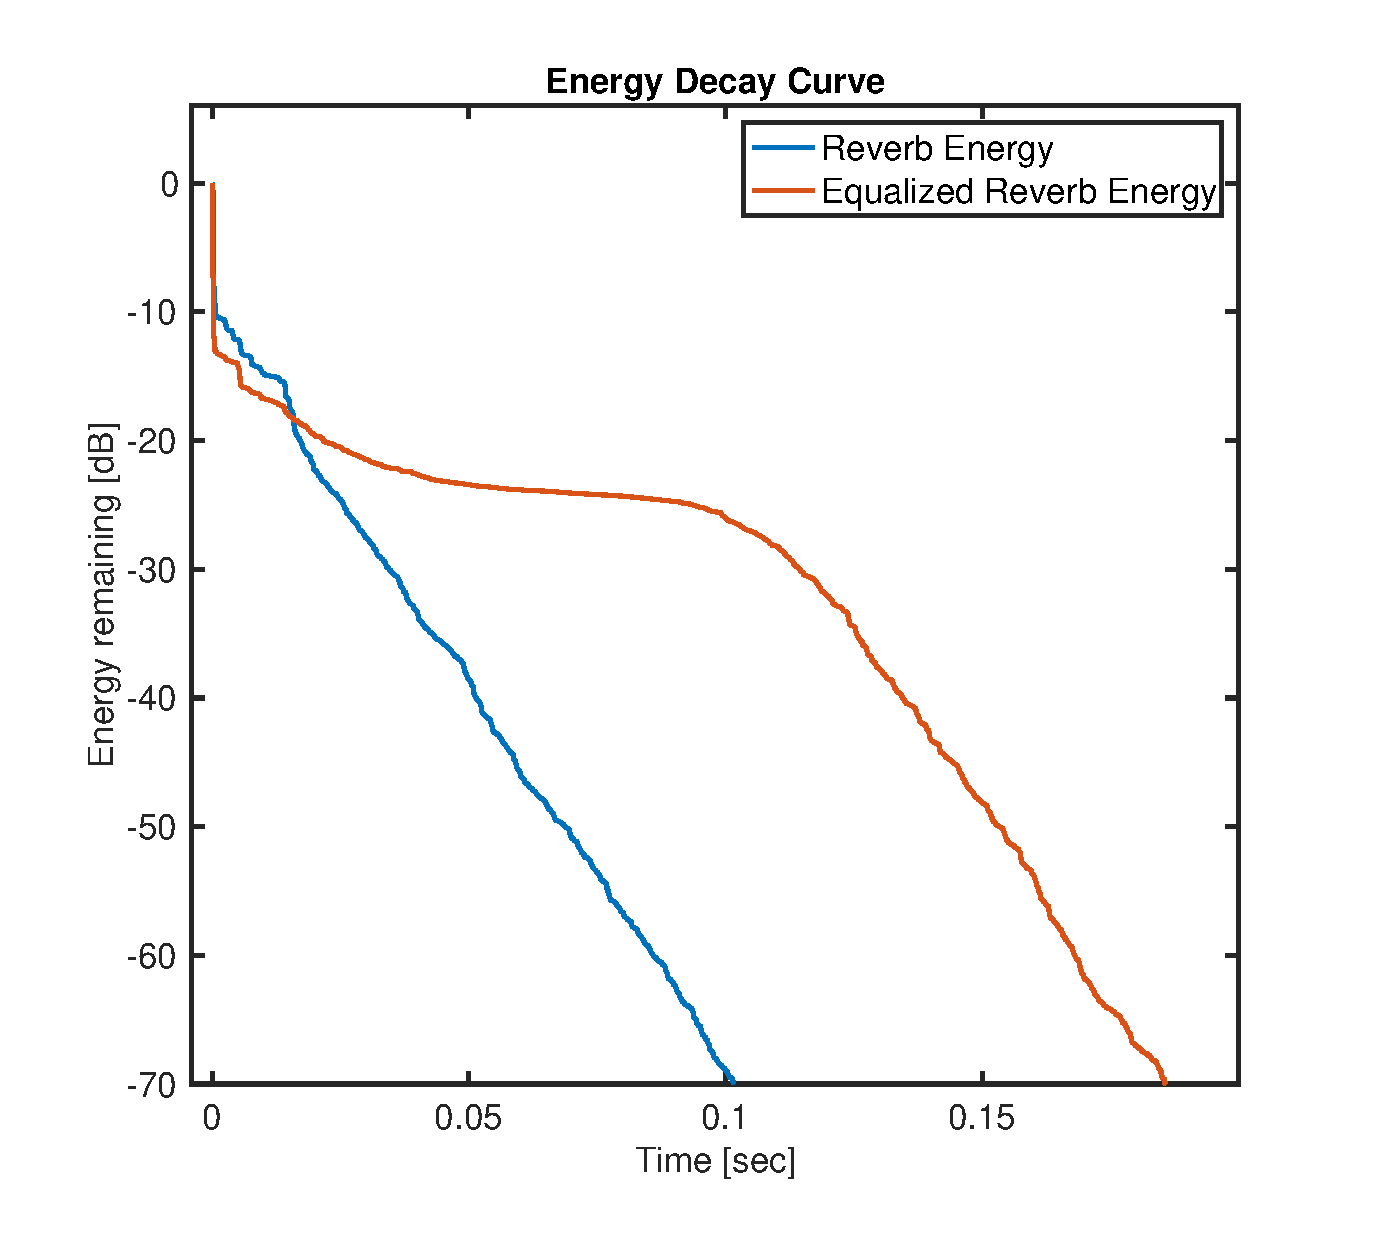
\includegraphics[width=\linewidth]{EDC_SourceLength_1_Blind}
			\end{subfigure}
		\end{minipage}
	}
	% Dummy subfigure for referencing row A
	\refstepcounter{subfigure}
	\label{subfig:params_source_length_compare:A}
	
	\vspace{1em}
	
	% ROW B
	\makebox[\textwidth][l]{%
		\begin{minipage}{0.08\textwidth}
			\centering
			\raggedleft{\footnotesize \textbf{(b)} \newline \qty{7.3}{\sec} \newline source} \\
		\end{minipage}%
		\begin{minipage}{0.91\textwidth}
			\begin{subfigure}[t]{0.32\textwidth}
				\centering
				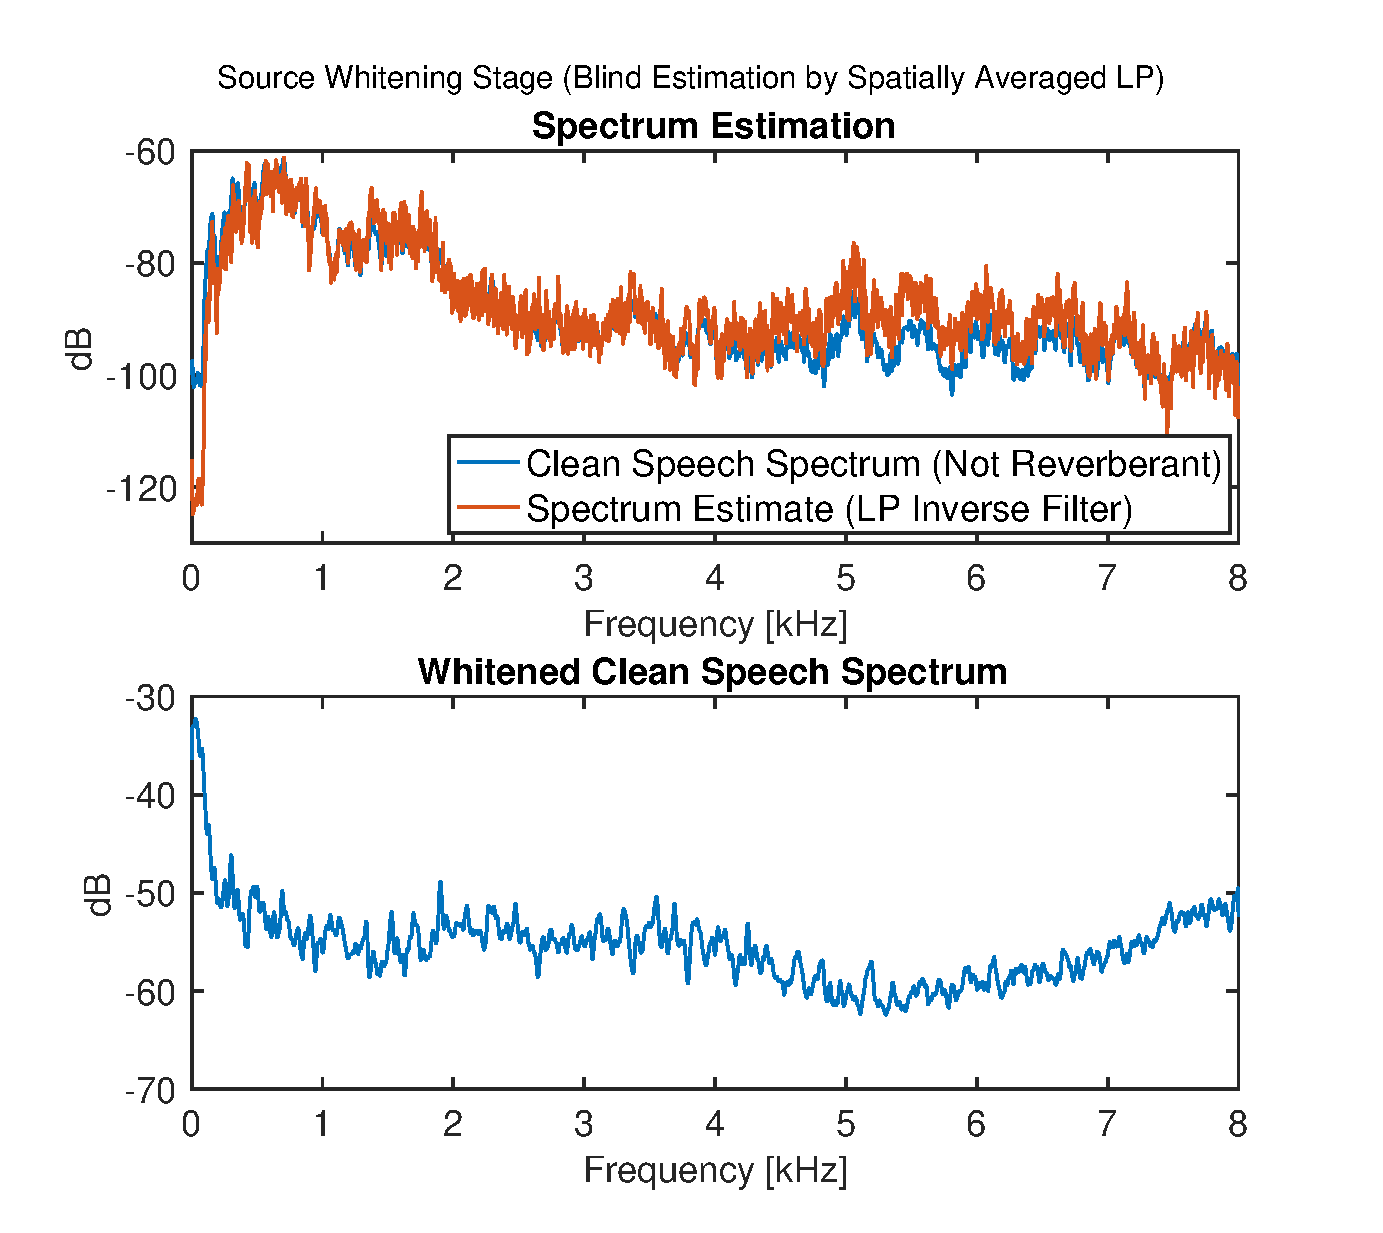
\includegraphics[width=\linewidth]{S1_SourceLength_2_Blind}
			\end{subfigure}
			\hfill
			\begin{subfigure}[t]{0.32\textwidth}
				\centering
				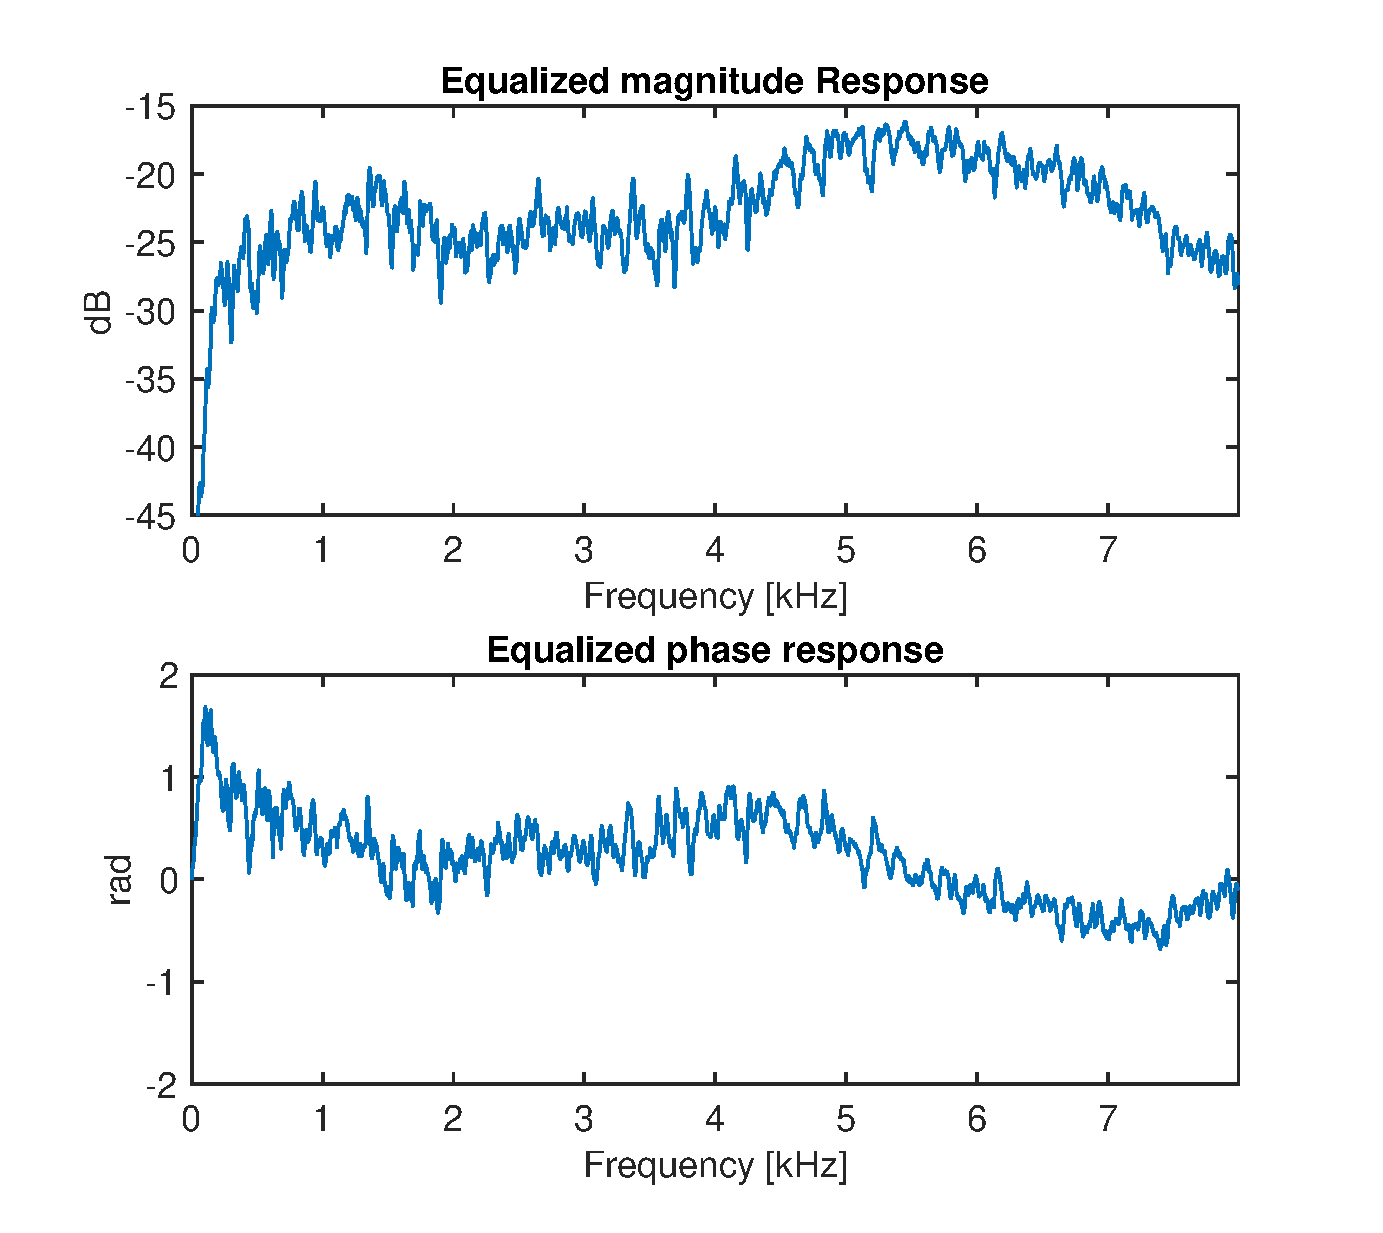
\includegraphics[width=\linewidth]{Equalized_RTF_SourceLength_2_Blind}
			\end{subfigure}
			\hfill
			\begin{subfigure}[t]{0.32\textwidth}
				\centering
				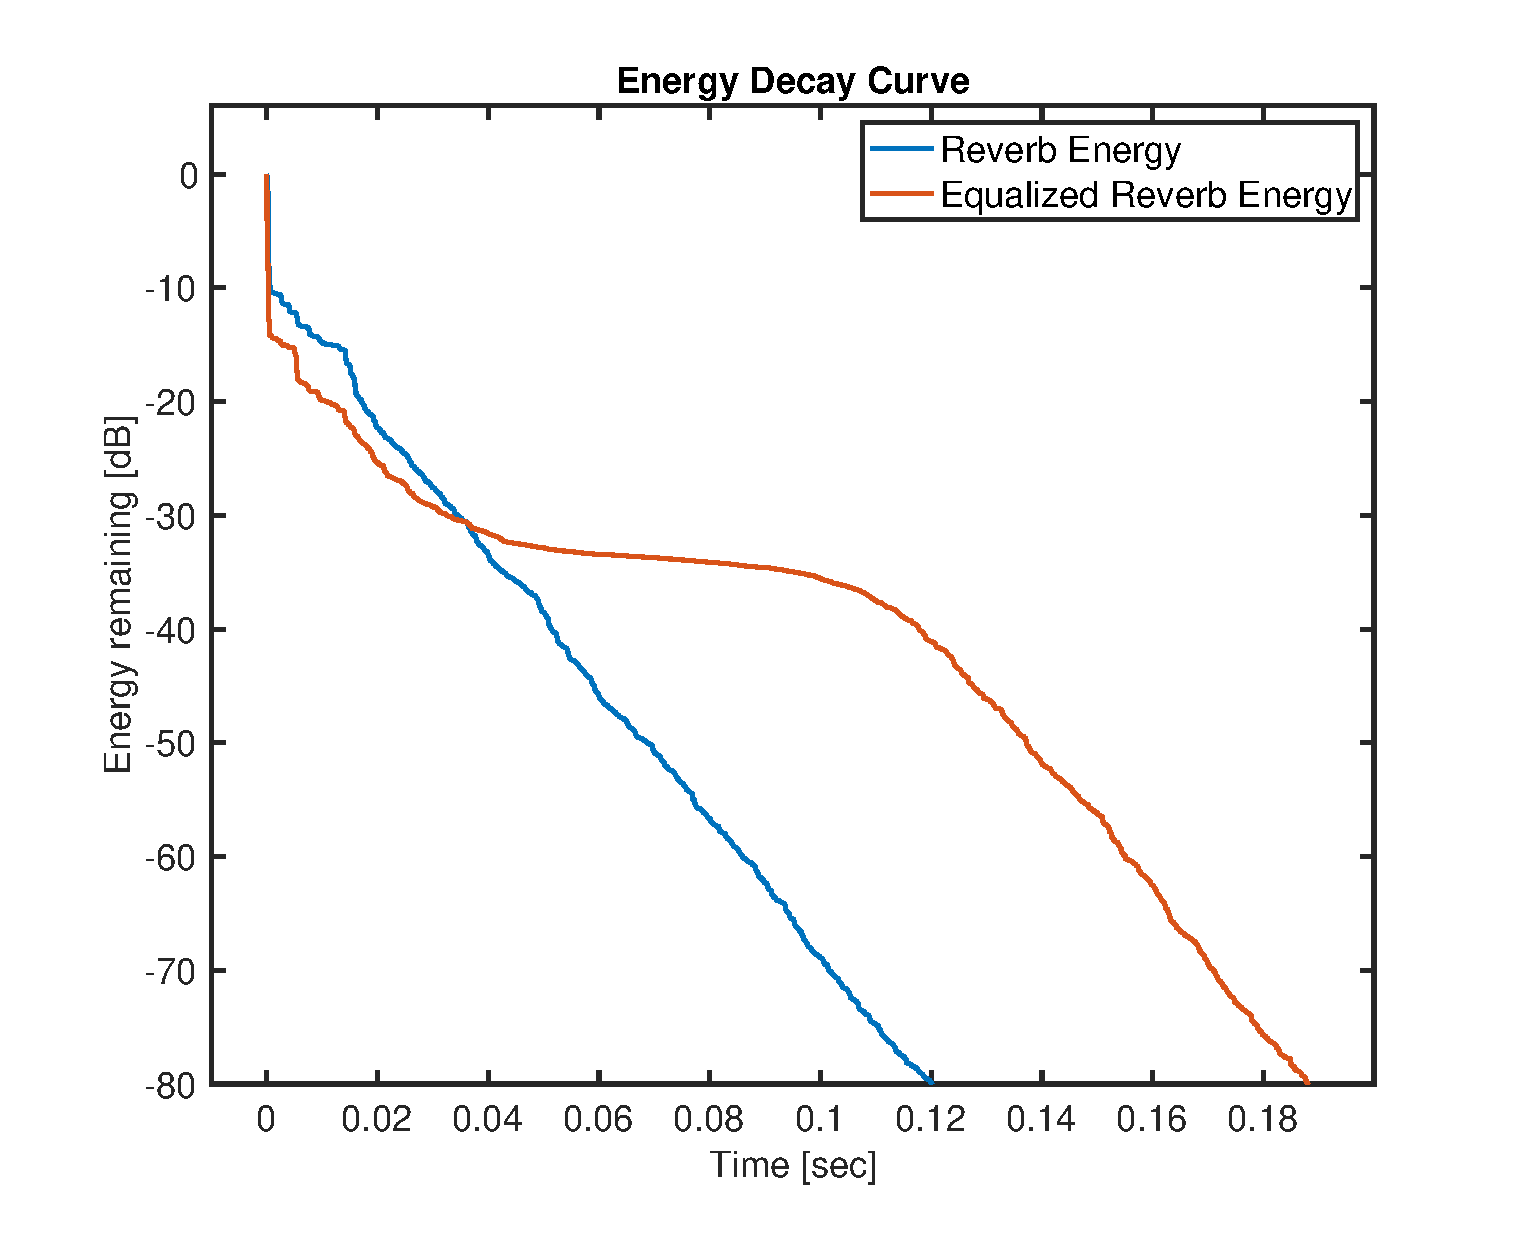
\includegraphics[width=\linewidth]{EDC_SourceLength_2_Blind}
			\end{subfigure}
		\end{minipage}
	}
	% Dummy subfigure for referencing row B
	\refstepcounter{subfigure}
	\label{subfig:params_source_length_compare:B}
	
	\vspace{1em}
	
	% ROW C
	\makebox[\textwidth][l]{%
		\begin{minipage}{0.08\textwidth}
			\centering
			\raggedleft{\footnotesize \textbf{(c)} \newline \qty{10.9}{\sec} \newline source} \\
		\end{minipage}%
		\begin{minipage}{0.91\textwidth}
			\begin{subfigure}[t]{0.32\textwidth}
				\centering
				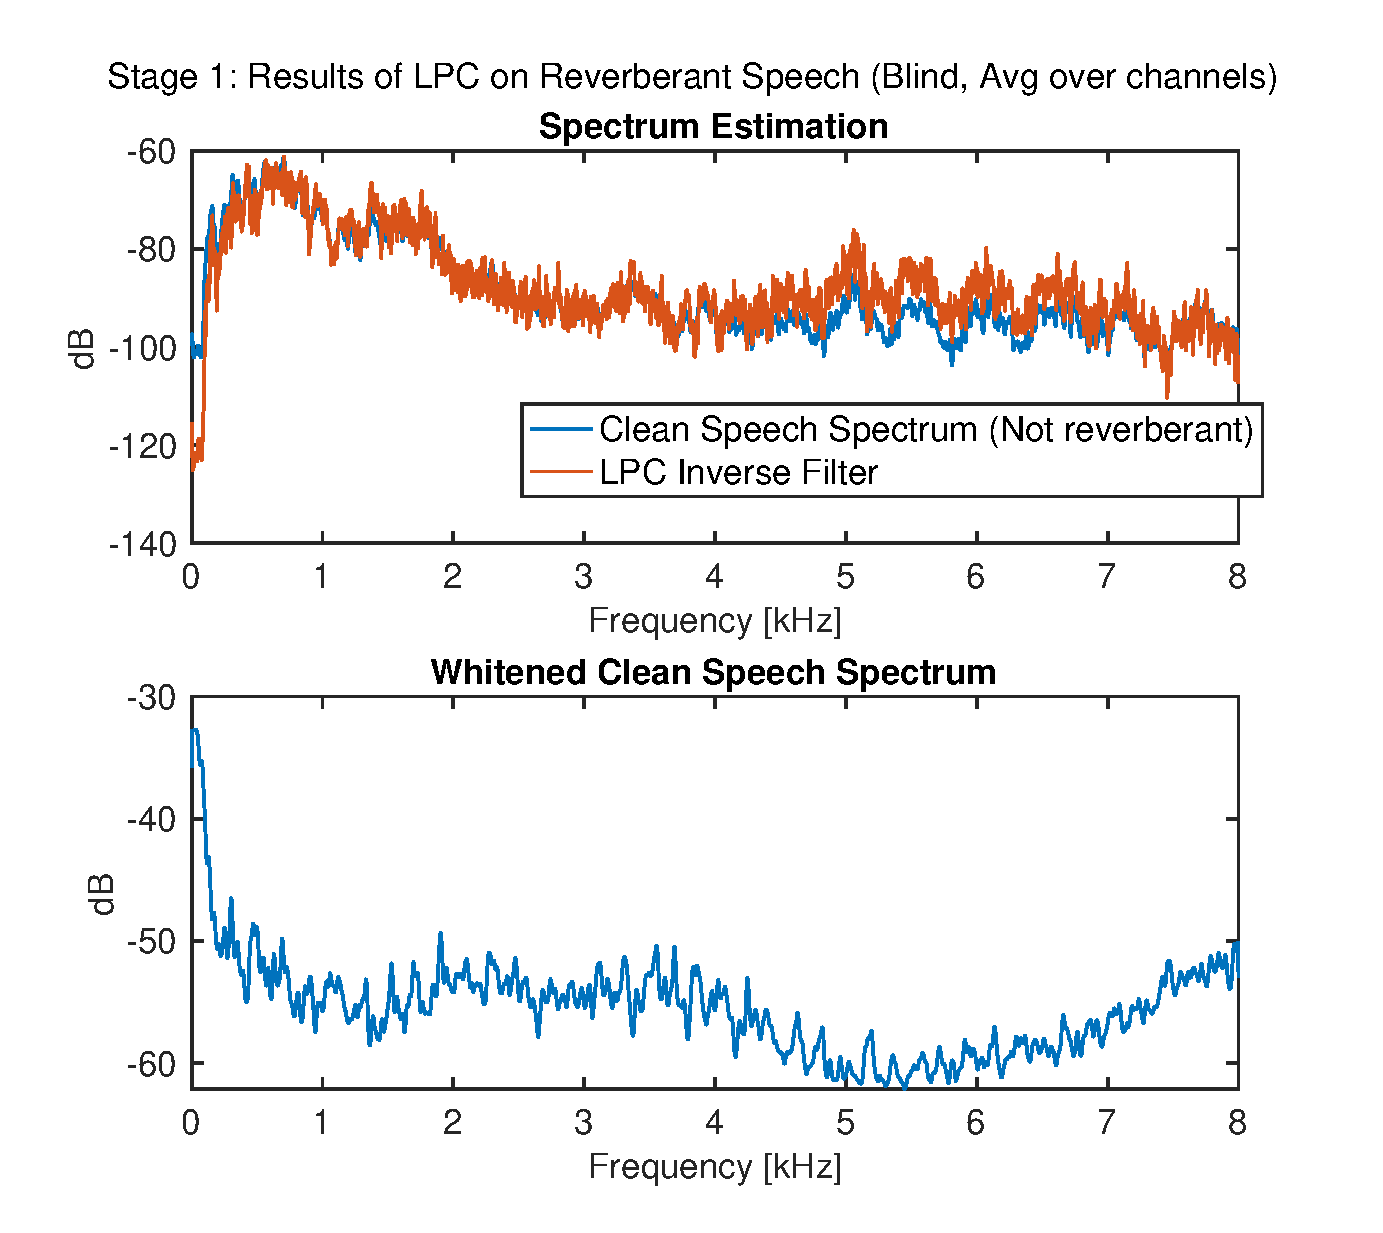
\includegraphics[width=\linewidth]{S1_SourceLength_3_Blind}
			\end{subfigure}
			\hfill
			\begin{subfigure}[t]{0.32\textwidth}
				\centering
				\includegraphics[width=\linewidth]{Equalized_RTF_SourceLength_3_Blind}
			\end{subfigure}
			\hfill
			\begin{subfigure}[t]{0.32\textwidth}
				\centering
				\includegraphics[width=\linewidth]{EDC_SourceLength_3_Blind}
			\end{subfigure}
		\end{minipage}
	}
	% Dummy subfigure for referencing row C
	\refstepcounter{subfigure}
	\label{subfig:params_source_length_compare:C}
	
	\vspace{1em}
	
	% ROW D
	\makebox[\textwidth][l]{%
		\begin{minipage}{0.08\textwidth}
			\centering
			\raggedleft{\footnotesize \textbf{(d)} \newline \qty{14.5}{\sec} \newline source} \\
		\end{minipage}%
		\begin{minipage}{0.91\textwidth}
			\begin{subfigure}[t]{0.32\textwidth}
				\centering
				\includegraphics[width=\linewidth]{S1_SourceLength_4_Blind}
			\end{subfigure}
			\hfill
			\begin{subfigure}[t]{0.32\textwidth}
				\centering
				\includegraphics[width=\linewidth]{Equalized_RTF_SourceLength_4_Blind}
			\end{subfigure}
			\hfill
			\begin{subfigure}[t]{0.32\textwidth}
				\centering
				\includegraphics[width=\linewidth]{EDC_SourceLength_4_Blind}
			\end{subfigure}
		\end{minipage}
	}
	% Dummy subfigure for referencing row D
	\refstepcounter{subfigure}
	\label{subfig:params_source_length_compare:D}
	
	\caption[Impact of source data length on DAP dereverberation performance]{Impact of source data length on DAP dereverberation performance. In each case, the same \qty{3.6}{\sec} speech sample (\qty{58}{\kilo samples} at $f_s=\qty{16}{\kilo\hertz}$) was looped to a different data length to preserve the same spectrum. Source whitening prediction order was $\mathrm{p_1} = 2 \cdot \mathrm{p_2} \cdot (M-1)$ and MC-LP order was $\mathrm{p_2} = \mathrm{N60} / (M-1)$. Source Whitening stage was performed on reverberant speech (i.e., blind estimation).}
	\label{fig:params_source_length_compare}
	
\end{figure}

Comparing the EDC results (third column in Figure \ref{fig:params_source_length_compare}), it is clear that the amount of source data used in training the algorithm has an impact on reverberation cancellation performance, independent of the source spectrum. Specifically, it was observed that the level at which the EDC plateaus (i.e., the point at which estimation variance is strong relative to reverberation as previously discussed) scales approximately from \qty{20}{\decibel} in Figure \ref{subfig:params_source_length_compare:A} to \qty{35}{\decibel} in Figure \ref{subfig:params_source_length_compare:D}. The dependency of performance on the amount of source data used in training makes sense because using more data decreases autocorrelation estmation variance which is a key limiting factor of performance. The difference in estimation variance  between the four cases is visible as subtle changes to the amount of ripples in the whitened source spectra and equalized magnitude/phase responses. Note that linear prediction in the context of traditional speech coding uses lower orders (often modeling as few as 8-16 poles), thus requiring far less data to sufficiently reduce estimation variance. 

%Additionally, in speech coding the goal is often to model only the more prominent spectral shape (i.e., the spectral envelope) and the smaller spectral details may be neglected. In dereverberation, the final details of the RTF, which are the frequency-dual of the later/weaker part of the RIR, are non-negligible as they contribute to the perceptual reverberance of the room. 

%Interestingly the increased estimation variance for smaller amounts of source data was only found to be visible in the source-whitening results and equalized RTF results (columns 1 and 2) in the first test case, i.e., Figure \ref{subfig:params_source_length_compare:A}. The variance is visible in this case as substantial ripples and deviation in the whitened clean speech spectrum, equalized magnitude response and equalized phase response. For larger training signal lengths, the difference in these plots were found to be less obvious, but the benefit was still visible in the EDC results as explained above.

The EDC benefit of increasing the amount of source data was observed to hit a ceiling over about \qty{10}{\sec} of data (i.e., over approximately \qty{160}{\kilo samples} for $f_s=\qty{16}{\kilo\hertz}$), which is highly dependent on the specific prediction orders used in this test. If the prediction orders were increased, more data would be needed to acheive the same performance. Therefore, the amount of data used in training the algorithm (i.e., used in the normal equations) should be selected as needed to minimize estimation variance for the selected prediction orders. However, in practice the amount of data used is limited by the time-varying nature of RTFs. An analysis window of \qty{10}{\sec} of data was used for the remainer of this thesis, since anything larger would be completely unreasonble to assume a stationary RTF. The massive amount of data needed severely impacts the ability of MC-LP approaches to reverberation cancellation to track time-varying acoustics.

\subsection{Source Spectrum}

To evaluate the impact of source spectrum, in each test case the source was produced by synthetically generating a random white noise sequence of a different length (\qty{100}{\milli\sec}, \qty{1}{\sec} and \qty{10}{\sec} respectively), then looping these sequences to the same length (a duration of \qty{60}{\sec}). Since shorter realizations of the same uncorrelated (white) random process have a higher degree of correlation, this results in sequences of the same length with controllable spectral dynamic range. The results for each case are shown in Figure \ref{fig:params_source_spectrum_compare}. The same four-channel RIR, and prediction orders were used as in the last section.

% Test: Same length different spectrum
% -     Blind DAP
% - 	Test: Speech is different length white noise sequences looped to length = 60 sec = 960000 (as original sequence length goes down, peakiness of spectrum goes up but final length doesn’t change)
% - 	RIR = SAL truncated to 100 msec = 1600 samples, M = 4 mics
% - 	P1 = 2 * p2 * (M-1)
% - 	P2 = N60 / (M-1)

% Source Spectrum Compare, Initial White noise sequence length = [0.1 sec 1 sec  10 sec], Blind
\begin{figure}[H]
	\centering
	
	% ROW A
	\makebox[\textwidth][l]{%
		\begin{minipage}{0.07\textwidth}
			\centering
			\raggedleft{\footnotesize \textbf{(a)} \newline \qty{0.1}{\sec} \newline white \newline noise} \\
		\end{minipage}%
		\begin{minipage}{0.92\textwidth}
			\begin{subfigure}[t]{0.32\textwidth}
				\centering
				\includegraphics[width=\linewidth]{S1_SourceSpectrum_100msecWhiteNoise_Blind}
			\end{subfigure}
			\hfill
			\begin{subfigure}[t]{0.32\textwidth}
				\centering
				\includegraphics[width=\linewidth]{Equalized_RTF_SourceSpectrum_100msecWhiteNoise_Blind}
			\end{subfigure}
			\hfill
			\begin{subfigure}[t]{0.32\textwidth}
				\centering
				\includegraphics[width=\linewidth]{EDC_SourceSpectrum_100msecWhiteNoise_Blind}
			\end{subfigure}
		\end{minipage}
	}
	% Dummy subfigure for referencing row A
	\refstepcounter{subfigure}
	\label{subfig:params_source_spectrum_compare:A}
	
	\vspace{1em}
	
	% ROW B
	\makebox[\textwidth][l]{%
		\begin{minipage}{0.07\textwidth}
			\centering
			\raggedleft{\footnotesize \textbf{(b)} \newline \qty{1}{\sec} \newline white \newline noise} \\
		\end{minipage}%
		\begin{minipage}{0.92\textwidth}
			\begin{subfigure}[t]{0.32\textwidth}
				\centering
				\includegraphics[width=\linewidth]{S1_SourceSpectrum_1secWhiteNoise_Blind}
			\end{subfigure}
			\hfill
			\begin{subfigure}[t]{0.32\textwidth}
				\centering
				\includegraphics[width=\linewidth]{Equalized_RTF_SourceSpectrum_1secWhiteNoise_Blind}
			\end{subfigure}
			\hfill
			\begin{subfigure}[t]{0.32\textwidth}
				\centering
				\includegraphics[width=\linewidth]{EDC_SourceSpectrum_1secWhiteNoise_Blind}
			\end{subfigure}
		\end{minipage}
	}
	% Dummy subfigure for referencing row B
	\refstepcounter{subfigure}
	\label{subfig:params_source_spectrum_compare:B}
	
	\vspace{1em}
	
	% ROW C
	\makebox[\textwidth][l]{%
		\begin{minipage}{0.07\textwidth}
			\centering
			\raggedleft{\footnotesize \textbf{(c)} \newline \qty{10}{\sec} \newline white \newline noise} \\
		\end{minipage}%
		\begin{minipage}{0.92\textwidth}
			\begin{subfigure}[t]{0.32\textwidth}
				\centering
				\includegraphics[width=\linewidth]{S1_SourceSpectrum_10secWhiteNoise_Blind}
			\end{subfigure}
			\hfill
			\begin{subfigure}[t]{0.32\textwidth}
				\centering
				\includegraphics[width=\linewidth]{Equalized_RTF_SourceSpectrum_10secWhiteNoise_Blind}
			\end{subfigure}
			\hfill
			\begin{subfigure}[t]{0.32\textwidth}
				\centering
				\includegraphics[width=\linewidth]{EDC_SourceSpectrum_10secWhiteNoise_Blind}
			\end{subfigure}
		\end{minipage}
	}
	% Dummy subfigure for referencing row C
	\refstepcounter{subfigure}
	\label{subfig:params_source_spectrum_compare:C}
	
	\caption[Impact of source signal spectrum on DAP dereverberation performance]{Impact of source signal spectrum on DAP dereverberation performance. The source signal in each case was generated by synthetically looping a different length white noise sequence to the same duration of \qty{60}{\sec} (i.e., same data length, different spectra). Source whitening prediction order was $\mathrm{p_1} = 2 \cdot \mathrm{p_2} \cdot (M-1)$ and MC-LP order was $\mathrm{p_2} = \mathrm{N60} / (M-1)$. Source Whitening stage was performed on revererbant speech (i.e., blind estimation).}
	\label{fig:params_source_spectrum_compare}
	
\end{figure}

As expected, reverberation cancellation performance was found to scale with how uncorrelated (i.e., white) the source signal was. As previously mentioned, this can potentially be attributed to two effects: the inverse proportionality between the conditioning of the normal equations and the spectral dynamic range of source signal, and the increased demand on the source-whitening stage as the source spectrum becomes more detailed (i.e., fine details of spectrum). To distinguish between these two explanations, an additional test was conducted whereby the source signals were generated by filtering the same white noise sequence with filters of varying peakiness. In this way, the fine details of the source spectrum were kept the same between tests, but the spectral dynamic range was varied.

% Source Spectrum Compare, Same 60 sec white noise sequence shaped with 3 filters of varying peakiness.
\begin{figure}[H]
	\centering
	
	% ROW A
	\makebox[\textwidth][l]{%
		\begin{minipage}{0.08\textwidth}
			\centering
			\raggedleft{\footnotesize \textbf{(a)} \newline Filter 1} \\
		\end{minipage}%
		\begin{minipage}{0.91\textwidth}
			\begin{subfigure}[t]{0.32\textwidth}
				\centering
				\includegraphics[width=\linewidth]{S1_SourceSpectrum_10secShapedNoise_filter1_Blind}
			\end{subfigure}
			\hfill
			\begin{subfigure}[t]{0.32\textwidth}
				\centering
				\includegraphics[width=\linewidth]{Equalized_RTF_SourceSpectrum_10secShapedNoise_filter1_Blind}
			\end{subfigure}
			\hfill
			\begin{subfigure}[t]{0.32\textwidth}
				\centering
				\includegraphics[width=\linewidth]{EDC_SourceSpectrum_10secShapedNoise_filter1_Blind}
			\end{subfigure}
		\end{minipage}
	}
	% Dummy subfigure for referencing row A
	\refstepcounter{subfigure}
	\label{subfig:params_source_spectrum_shaped_compare:A}
	
	\vspace{1em}
	
	% ROW B
	\makebox[\textwidth][l]{%
		\begin{minipage}{0.08\textwidth}
			\centering
			\raggedleft{\footnotesize \textbf{(b)} \newline Filter 2} \\
		\end{minipage}%
		\begin{minipage}{0.91\textwidth}
			\begin{subfigure}[t]{0.32\textwidth}
				\centering
				\includegraphics[width=\linewidth]{S1_SourceSpectrum_10secShapedNoise_filter2_Blind}
			\end{subfigure}
			\hfill
			\begin{subfigure}[t]{0.32\textwidth}
				\centering
				\includegraphics[width=\linewidth]{Equalized_RTF_SourceSpectrum_10secShapedNoise_filter2_Blind}
			\end{subfigure}
			\hfill
			\begin{subfigure}[t]{0.32\textwidth}
				\centering
				\includegraphics[width=\linewidth]{EDC_SourceSpectrum_10secShapedNoise_filter2_Blind}
			\end{subfigure}
		\end{minipage}
	}
	% Dummy subfigure for referencing row B
	\refstepcounter{subfigure}
	\label{subfig:params_source_spectrum_shaped_compare:B}
	
	\vspace{1em}
	
	% ROW C
	\makebox[\textwidth][l]{%
		\begin{minipage}{0.08\textwidth}
			\centering
			\raggedleft{\footnotesize \textbf{(c)} \newline Filter 3} \\
		\end{minipage}%
		\begin{minipage}{0.91\textwidth}
			\begin{subfigure}[t]{0.32\textwidth}
				\centering
				\includegraphics[width=\linewidth]{S1_SourceSpectrum_10secShapedNoise_filter3_Blind}
			\end{subfigure}
			\hfill
			\begin{subfigure}[t]{0.32\textwidth}
				\centering
				\includegraphics[width=\linewidth]{Equalized_RTF_SourceSpectrum_10secShapedNoise_filter3_Blind}
			\end{subfigure}
			\hfill
			\begin{subfigure}[t]{0.32\textwidth}
				\centering
				\includegraphics[width=\linewidth]{EDC_SourceSpectrum_10secShapedNoise_filter3_Blind}
			\end{subfigure}
		\end{minipage}
	}
	% Dummy subfigure for referencing row C
	\refstepcounter{subfigure}
	\label{subfig:params_source_spectrum_shaped_compare:C}
	
	\caption[Impact of source spectral dynamic range on DAP dereverberation performance]{Impact of source spectral dynamic range on DAP dereverberation performance. The source signal was generated by filtering \qty{60}{\milli\sec} of speech with filters of various peakiness. Source whitening prediction order was $\mathrm{p_1} = 2 \cdot \mathrm{p_2} \cdot (M-1)$ and MC-LP was $\mathrm{p_2} = \mathrm{N60} / (M-1)$. Source Whitening stage was performed on revererbant speech (i.e., blind estimation).}
	\label{fig:params_source_spectrum_shaped_compare}
	
\end{figure}

As shown in Figure \ref{fig:params_source_spectrum_shaped_compare}, the spectral dynamic range alone has very minimal impact on performance. This makes sense because the normal equations are constructed using the reverberant microphone signals, not the clean speech. RTFs are known to have strong notches and resonances, thus reverberant signals tend to have a large spectral dynamic range irrespective of the source signal spectrum. Thus it was concluded that the primary spectral characteristic of the source signal that impacts performance is the complexity of fine spectral details, which make the job of the source-whitening stage more difficult.


\section{Time Alignment of RIRs and Linear Combiner}

To evaluate the influence of time alignment of the RIRs on dereverberation performance, the DAP algorithm was run excluding the diagonal delay matrix, $\boldsymbol{D}(z)$. The four RIRs were generated synthetically by applying an exponentially decaying window to a Gaussian white noise sequence and then were maually delayed to misalign them. Figure \ref{fig:params_MC_EIR_TimeAlignment_0sampleDelay} shows the results when the RIRs are time aligned, and Figure \ref{fig:params_MC_EIR_TimeAlignment_2sampleDelay} shows the results when an incremental delay of two samples was introduced accross the microphones. The delay increases from channel 1 to channel 4, i.e., channel 1 leads all other channels. The left column of the results plots shows RIRs for each channel. The right column shows the four EIRs prior to linear combination, i.e., the vector-valued EIR $\boldsymbol{\mathrm{eir}}(z)$ excluding the linear combiner vector, i.e.,

\begin{equation}
	\boldsymbol{\mathrm{eir}}(z) = \boldsymbol{g}(z)\boldsymbol{A}_{pe,mc}(z) = \begin{bmatrix} \mathrm{eir}_1 (z)& \dots & \mathrm{eir}_M(z) \end{bmatrix}^T
\end{equation}

\noindent
where $\boldsymbol{g}(z) = \begin{bmatrix} G_1(z)& \dots & G_M(z) \end{bmatrix}^T$ is the vector-valued $M$-channel RTF.

%Test:
% - Synthetic RIRs, delayed manually (incremental delay added per channel), T60=100msec
% - L channel = N60 * 2 = 3200 samples (~120 dB attenuation)
% - Source = SA1.wav looped for 20 sec
% - S1 on clean speech
% - Figures saved (.fig)


\begin{figure}[H]
	\includegraphics[width=0.8\textwidth]{MC_EIR_TimeAlignment_0sampleDelay}
	\centering
	\caption[DAP dereverberation performance pre-linear combiner for time-aligned RIRs]{Vector-valued EIR performance prior to linear combiner with no time delay between channels (i.e., time aligned).}
	\label{fig:params_MC_EIR_TimeAlignment_0sampleDelay}
\end{figure}

\begin{figure}[H]
	\includegraphics[width=0.8\textwidth]{MC_EIR_TimeAlignment_2sampleDelay}
	\centering
	\caption[DAP dereverberation performance pre-linear combiner for non time-aligned RIRs]{Vector-valued EIR performance prior to linear combiner with an incremental 2-sample delay added to each channel (i.e., not time aligned).}
	\label{fig:params_MC_EIR_TimeAlignment_2sampleDelay}
\end{figure}


From Figure \ref{fig:params_MC_EIR_TimeAlignment_0sampleDelay}, note that all four individual EIRs show an impulse-like shape, suggesting reasonable equalization. However, in Figure \ref{fig:params_MC_EIR_TimeAlignment_2sampleDelay}, it was observed that whenever the signal being predicted by the MC-LP stage lags the other signals, the signal is eliminated instead of the channel being equalized (i.e., the EIR is all zeros instead of becoming impulse-like). This is an expected behavior of MC-LP since the whitening nature of linear prediction is reliant on the signal only being estimated strictly from past samples. If channel 2 lags channel 1 by samples, prediction of channel 2 from channel 1 will have access to current source information, thus being able to perfectly cancel it instead of only whitening. Additionally, when predicting the channel that leads the rest (thus remaining a whitening process), the lack of time alignment still negatively impacts performance, which is evident from the burst of unequalized reverberation in the row 1 EIR from Figure \ref{fig:params_MC_EIR_TimeAlignment_2sampleDelay}. Time alignment has a clear impact on dereverberation performance after linear combination as well, as shown in Figure \ref{fig:params_TimeAlignment_0sampleDelay} and Figure \ref{fig:params_TimeAlignment_2sampleDelay} below.


\begin{figure}[H]
	\centering
	\begin{subfigure}[b]{0.32\textwidth}
		\centering
		\includegraphics[width=\textwidth]{EIR_TimeAlignment_0sampleDelay}
	\end{subfigure}
	\hfill
	\begin{subfigure}[b]{0.32\textwidth}
		\centering
		\includegraphics[width=\textwidth]{Equalized_RTF_TimeAlignment_0sampleDelay}
	\end{subfigure}
	\hfill
	\begin{subfigure}[b]{0.32\textwidth}
		\centering
		\includegraphics[width=\textwidth]{EDC_TimeAlignment_0sampleDelay}
	\end{subfigure}
	\hfill
	\caption[DAP dereverberation performance for time-aligned RIRs]{DAP dereverberation performance (after linear combiner) with no time delay between channels (i.e., time aligned)}
	\label{fig:params_TimeAlignment_0sampleDelay}
\end{figure}

\begin{figure}[H]
	\centering
	\begin{subfigure}[b]{0.32\textwidth}
		\centering
		\includegraphics[width=\textwidth]{EIR_TimeAlignment_2sampleDelay}
	\end{subfigure}
	\hfill
	\begin{subfigure}[b]{0.32\textwidth}
		\centering
		\includegraphics[width=\textwidth]{Equalized_RTF_TimeAlignment_2sampleDelay}
	\end{subfigure}
	\hfill
	\begin{subfigure}[b]{0.32\textwidth}
		\centering
		\includegraphics[width=\textwidth]{EDC_TimeAlignment_2sampleDelay}
	\end{subfigure}
	\hfill
	\caption[DAP dereverberation performance for non time-aligned RIRs]{DAP dereverberation performance (after linear combiner) with an incremental 2-sample delay added to each channel (i.e., not time aligned).}
	\label{fig:params_TimeAlignment_2sampleDelay}
\end{figure}

The linear combiner used ($\boldsymbol{g}_0$) was the estimate of the first vector coefficient of the SIMO channel, as proposed by \cite{triki2006delay} and as discussed in Section \ref{section_dap}. From this analysis, the motivation for using this linear combiner is evident: a larger scalar element from the vector $\boldsymbol{g}_0$ implies that the corresponding channel leads the others and as such will act as a whitening filter, which is desired, and not a signal cancellation filter. Thus this linear combiner method puts larger weights on the EIRs that are impulse-like and therefore provides some protection against poor time alignment. For the remainder of this thesis, the RIRs were manually time aligned, but this linear combination method was still used.

\section{Algorithmic Complexity Analysis} \label{section:complexity}

An important consideration in selecting the linear prediction orders for the source-whitening and MC-LP stages is the memory and computational requirements required to implement the algorithm. Figure \ref{fig:complexity_operations} and Figure \ref{fig:complexity_memory} show how the required mathematical operations and memory scale with these parameters. The x-axis for these plots is T60, and the prediction orders used for each T60 are given by $p_2 = 0.75 \cdot N60 / \left(M-1\right)$ and $p_1 = 1.25 \cdot p_2 \cdot \left(M-1\right)$. These prediction orders were selected based on acheiving maximum performance for the given T60, as per the discussion in Section \ref{section:params_p2_MC_LP} and Section \ref{section:params_p1}. As such, the plots may be interpreted as showing the memory/computations required to provide maximum dereverberation performance for RIRs up to the given T60. These plots were generated assuming $M=4$ microphones, a sample rate of \qty{16}{\kilo\hertz} and a 32 bits of numerical precision.

\begin{figure}[H]
	\centering
	\begin{subfigure}[b]{0.45\textwidth}
		\centering
		\includegraphics[width=\textwidth]{complexity_ops_comparison}
	\end{subfigure}
	\hfill
	\begin{subfigure}[b]{0.45\textwidth}
		\centering
		\includegraphics[width=\textwidth]{complexity_ops_comparison_zoomed}
	\end{subfigure}
	\caption[DAP algorithm complexity (cycles)]{Analysis of the computational complexities of Least Squares solution and Inverse filter implementations as a function of T60, For $M=4$ microphones, $\mathrm{p_2} = 0.75 \cdot \mathrm{N60}/(M-1)$ and $\mathrm{p_1} = 1.25 \cdot \mathrm{p_2} \cdot (M-1)$. Complexity of LMS Solution also shown for comparison.}
	\label{fig:complexity_operations}
\end{figure}

\begin{figure}[H]
	\centering
	\begin{subfigure}[b]{0.45\textwidth}
		\centering
		\includegraphics[width=\textwidth]{complexity_mem_comparison}
	\end{subfigure}
	\hfill
	\begin{subfigure}[b]{0.45\textwidth}
		\centering
		\includegraphics[width=\textwidth]{complexity_mem_comparison_zoomed}
	\end{subfigure}
	\caption[DAP algorithm complexity (memory)]{Analysis of the algorithmic memory requirements  of Least Squares solution (could be temporary memory) and Inverse filter implementations (persistent memory) as a function of T60, For M=4 microphones, $\mathrm{p_2} = 0.75 \cdot \mathrm{N60}/(M-1)$ and $\mathrm{p_1} = 1.25 \cdot \mathrm{p_2} \cdot (M-1)$. Memory requirements of LMS Solution also shown for comparison.}
	\label{fig:complexity_memory}
\end{figure}

Both memory and computations associated with solving the normal equations scale exponentially with the T60 up to which we wish to optimally cancel. Equalizing RIRs up to a T60 of \qty{2}{\sec} requires approximately \qty{5e9}{operations} and  \qty{8}{\giga\byte} of memory, which is completely unrealistic in any practical system. Therefore for the purposes of the experiments in this thesis, it was decided to choose prediction orders to equalize RIRs up to a \qty{1}{\sec} T60, which requires approximately \qty{1e9}{operations} and \qty{2}{\giga\byte} of memory. This may be realistic in systems with tremendous amounts of processing power and memory, but is still completely unrealistic in an embedded application such as a hearing aid. To implement the algorithm in a more constrained system, the prediction orders would have to be reduced signficantly. This is a severe limitation of the algorithm, and presents a motivation for the to enhance the algorithm with other reverberation suppression techniques in any practical system. Another approach to reduce algorithmic complexity would be to estimate the source-whitening and MC-LP filters using an adaptive algorithm such as LMS instead of directly solving the normal equations. Unlike the normal equations solution, LMS updates scale linearly with prediction order, only requiring approximately \qty{4.5e4}{operations} and \qty{250}{\kilo\byte} for $\mathrm{T60} = \qty{1}{\sec}$, which could be improved further by using frequency/subband-domain adaptation. Using an adaptive algorithm would of course come at a cost of worse performance, but could potentially do a better job of tracking time varying acoustics. This was left for a future study.


\section{Conclusions} \label{section:params_conclusion}

To summarize, a number of parameters of the DAP algorithm and signal properties were investigated in terms of their influence on dereverberation performance: 

\begin{enumerate}
	\item \textbf{Multichannel Linear Prediction Order} ($p_2$): While in theory, near-perfect equalization of a length-$L$ RIR is possible with $p_2 = L / \left(M-1\right)$, in practice no additional performance gain was found for approximately $p_2 > 0.75 \cdot \mathrm{N60} / \left(M-1\right)$. In particular it was noted that there was always an increase in residual reverberation towards the end of the RIR. This limitation was assumed to be due to autocorrelation estimation variance at longer reverberation times due to limited signal data and the low energy of the late reflections. In practice it was found that the supervised DAP equalizer and the blind DAP equalizer were only able to acheive up to approximately \qty{35}{\decibel} and \qty{8}{\decibel} of reverberation suppression respectively under ideal conditions. While $p_2=\mathrm{N60}/\left(M-1\right)$ seems to be a reasonable prediction order, it will be shown in Section \ref{section:dap_eval_truncSAL} that for higher T60s the amount of data needed to reduce autocorrelation estimation variance becomes increasingly a limiting factor.
	
	 %$p_2=\mathrm{N60}/\left(M-1\right)$ will be used for experiments in this thesis. 
	%
	\item \textbf{Source Whitening Linear Prediction Order} ($p_1$): It was found that it was important to set $p_1 > p_2 \cdot \left(M-1\right)$ to match the spectral resolution of the source-whitening filter to the ``effective spectral resolution" of the MC-LP prediction error filter. $p_1 = 1.25 \cdot p_2 \cdot \left(M-1\right)$ was found to be reasonable.
	%
	\item \textbf{Number of Microphones} ($M$): Using more microphones was found to strongly improve blind estimation of the AR properties of the source which greatly improves performance. This is limited however by microphones available in the target system, and computations increase with number of microphones.
	%
	\item \textbf{Source Data Length}: A significant amount of data was found to be needed to bring down the estimation variance of the larger autocorrelation lags. For a sample rate of \qty{16}{\kilo\hertz} and T60 of \qty{100}{\milli\sec} (with prediction orders set as above), no improvement was seen for over approximately \qty{10}{\sec} of data, but this is expected to scale with T60. However the amount of data used in training is limited by the time varying nature of RTFs. A training signal of \qty{10}{\sec} will be used for experiments in this thesis.
	%
	\item \textbf{Source Spectrum}: The spectrum of the source signal was found to have a strong influence on dereverberation performance. In particular it was found that the density of fine spectral details had a negative impact on performance. This was assumed to be due to the increased demand on the source-whitening stage and the challenge of blindly estimating a complex source spectrum by spatial autocorrelation averaging accross microphones.
	%
	\item \textbf{Time Alignment of RIRs}: The time-alignment of the RIRs (and equivalentally of the microphone signals) was found to be crucial to algorithm performance. Without aligning the RIRs, the basic formulation of linear prediction being the prediction of current signal samples from only past signal samples breaks down, and the prediction error filters become cancellation filters instead of whitening filters. For the purposes of this thesis, the RIRs will be manually time-aligned and this procedure was left for future studies.
	%
	\item \textbf{Linear Combiner} ($\boldsymbol{g}_0$): The linear combiner proposed by \cite{triki2006delay} was investaged and it was shown that this technique provides some protection against time-alignment issues. This linear combiner will be used for the remainder of this thesis.
\end{enumerate}

Additionally, the memory and computational requirements were investigated and found to severly limit the practical applicability of DAP dereverberation. For the experiments in this thesis, the prediction orders were set initially to maximally cancel T60s up to \qty{1}{\sec} (i.e., $p_2=\mathrm{N60}/\left(M-1\right)=5333$ and $p_1 = 1.25 \cdot p_2 \cdot \left(M-1\right) = 20000$, for $f_s=\qty{16}{\kilo\hertz}).

%,  with $\mathrm{N60} = \mathrm{T60} \cdot \mathrm{sample \; rate}$, $\mathrm{T60} = \qty{1}{\sec}$).